% ============================================================
%  CP-Lib —— 算法竞赛模板库（打印版）
%
%  编译：  latexmk print/main.tex          （仓库根目录，.latexmkrc 已固化参数）
%     或：  cd print && latexmk main.tex
%
%  引擎必须是 XeLaTeX（文档含中文）。改用 pdflatex 会直接失败。
%
%  内容在各 chapters/*.tex 里，直接手改即可；那些 .tex 是打印版的正本。
% ============================================================
\documentclass[10pt,a4paper]{ctexart}

% ============================================================
%  CP-Lib 打印版 —— 导言区
%  引擎：XeLaTeX（中文必需）。用 latexmk -xelatex 编译。
% ============================================================

% ---------- 页面：A4 纵向，双栏，窄边距 ----------
% top 必须容纳 headheight + headsep，否则页眉会被裁掉
\usepackage[a4paper,top=13mm,bottom=12mm,left=9mm,right=9mm,headheight=13pt,headsep=3.5mm]{geometry}
\usepackage{multicol}

% ---------- 字体 ----------
% ctexart 已自动加载 xeCJK 并选用 Windows 字体（SimSun/SimHei/KaiTi）。
% 代码块里的中文注释走 \CJKttfamily，这里显式指定为宋体，小字号下最清晰。
\setCJKmonofont{SimSun}
% 拉丁等宽字体用于代码；Consolas 是 Windows 自带、比赛环境常见
\setmonofont{Consolas}[Scale=0.92]

% ---------- 数学 ----------
\usepackage{amsmath}
\usepackage{amssymb}
% CP-Lib.md 第 3565 行用了 $180\degree$，而 \degree 并非 base LaTeX/amsmath 提供，
% 不定义会直接编译失败。这里补上。
\newcommand{\degree}{\ensuremath{^{\circ}}}

% ---------- 标题层级压缩（双栏下必须，否则标题吃掉大量版面）----------
\usepackage{titlesec}
\usepackage{titletoc}

% h1 -> \section
\titleformat{\section}
  {\normalfont\large\bfseries\color{seccolor}}
  {\thesection}{0.6em}{}
\titlespacing*{\section}{0pt}{7pt}{3pt}

% h2 -> \subsection
\titleformat{\subsection}
  {\normalfont\normalsize\bfseries\color{subseccolor}}
  {\thesubsection}{0.5em}{}
\titlespacing*{\subsection}{0pt}{5pt}{2pt}

% h3 -> \subsubsection
\titleformat{\subsubsection}
  {\normalfont\small\bfseries}
  {\thesubsubsection}{0.5em}{}
\titlespacing*{\subsubsection}{0pt}{4pt}{1.5pt}

% h4 -> \paragraph（不编号，紧凑）
\titleformat{\paragraph}[runin]
  {\normalfont\small\bfseries}
  {}{0em}{}
\titlespacing*{\paragraph}{0pt}{3pt}{0.5em}

% 目录：收 h1/h2/h3
\setcounter{tocdepth}{3}
\setcounter{secnumdepth}{3}
\contentsmargin{1.6em}
\titlecontents{section}[0em]{\vspace{1pt}\bfseries}{\thecontentslabel\quad}{}{\titlerule*[0.4pc]{.}\contentspage}
\titlecontents{subsection}[1.2em]{\vspace{0.5pt}}{\thecontentslabel\quad}{}{\titlerule*[0.4pc]{.}\contentspage}
\titlecontents{subsubsection}[2.9em]{\small}{\thecontentslabel\quad}{}{\titlerule*[0.4pc]{.}\contentspage}

% ---------- 颜色 ----------
\usepackage{xcolor}
\definecolor{seccolor}{RGB}{0,0,0}
\definecolor{subseccolor}{RGB}{20,20,20}
\definecolor{codekw}{RGB}{0,0,190}
\definecolor{codecmt}{RGB}{0,120,0}
\definecolor{codestr}{RGB}{170,20,20}
\definecolor{codenum}{RGB}{140,0,140}
\definecolor{coderule}{RGB}{190,190,190}
\definecolor{linkcolor}{RGB}{0,0,200}

% ---------- 代码高亮 ----------
\usepackage{listings}
\lstset{
  language=C++,
  basicstyle=\ttfamily\scriptsize,
  keywordstyle=\color{codekw}\bfseries,
  commentstyle=\color{codecmt}\itshape,
  stringstyle=\color{codestr},
  numberstyle=\tiny\color{gray},
  % 折行：代码行宽 p99 约 85 列，单栏约容纳 69 列，超长行必须折
  breaklines=true,
  breakatwhitespace=false,
  breakindent=1em,
  % 注意：prebreak/postbreak 位于 \discretionary 内，其中不能出现 whatsit
  % （\color 会产生 whatsit），否则报 "Improper discretionary list"。故用 \raisebox。
  prebreak=\raisebox{0ex}[0ex][0ex]{\ensuremath{\searrow}},
  postbreak=\raisebox{0ex}[0ex][0ex]{\ensuremath{\hookrightarrow\space}},
  columns=fullflexible,
  keepspaces=true,
  showstringspaces=false,
  tabsize=4,
  extendedchars=true,
  frame=l,
  framerule=0.4pt,
  rulecolor=\color{coderule},
  xleftmargin=1.4mm,
  xrightmargin=0.4mm,
  framexleftmargin=0.4mm,
  aboveskip=4pt,
  belowskip=3pt,
  % 超长代码块允许跨栏/跨页断开
  breakautoindent=true,
}

% ---------- 页眉页脚（页码）----------
\usepackage{fancyhdr}
\usepackage{lastpage}
\pagestyle{fancy}
\fancyhf{}
\renewcommand{\headrulewidth}{0.3pt}
\renewcommand{\footrulewidth}{0pt}
\renewcommand{\sectionmark}[1]{\markboth{#1}{}}
\fancyhead[L]{\small\nouppercase{\leftmark}}
\fancyhead[R]{\small\itshape CP-Lib}
\fancyfoot[C]{\small\thepage\ /\ \pageref{LastPage}}

% ---------- 图片、链接 ----------
\usepackage{graphicx}
\usepackage[hidelinks]{hyperref}
\hypersetup{
  colorlinks=true,
  linkcolor=linkcolor,
  urlcolor=linkcolor,
  bookmarksnumbered=true,
  pdftitle={CP-Lib 算法竞赛模板},
  pdfsubject={算法竞赛模板库},
}

% ---------- 列表 ----------
\usepackage{enumitem}
\setlist[itemize]{topsep=2pt,itemsep=1pt,parsep=0pt,leftmargin=1.2em}
\setlist[enumerate]{topsep=2pt,itemsep=1pt,parsep=0pt,leftmargin=1.6em}

% ---------- 正文排版 ----------
\usepackage{indentfirst}
\setlength{\parindent}{0pt}
\setlength{\parskip}{2pt}
\linespread{1.04}


\begin{document}

% ---------------- 首页标题 ----------------
\thispagestyle{empty}
\begin{center}
  \vspace*{2mm}
  {\Huge\bfseries CP-Lib}\\[3mm]
  {\large 算法竞赛模板库}\\[2mm]
  {\small 封装式模板 · 快速复用}
\end{center}
\vspace{3mm}

% ---------------- 目录 ----------------
\begin{multicols}{2}
\tableofcontents
\end{multicols}

\clearpage

% ---------------- 正文（双栏通排）----------------
\begin{multicols}{2}

\section{图论}

\subsection{拓扑排序}

\begin{lstlisting}
#include <bits/stdc++.h>
using namespace std;

/**
 * @brief 拓扑排序封装
 * 适用场景：有向无环图（DAG）的先后顺序处理，检测环。
 */
struct TopoSort {
    int n;
    vector<int> in;          // 入度数组
    vector<vector<int>> g;   // 邻接表

    TopoSort(int n) : n(n), in(n + 1, 0), g(n + 1) {}

    void add_edge(int u, int v) {
        g[u].push_back(v);
        in[v]++;
    }

    vector<int> solve() {
        queue<int> q;
        vector<int> res;
        for (int i = 1; i <= n; i++)
            if (in[i] == 0) q.push(i);

        while (!q.empty()) {
            int u = q.front(); q.pop();
            res.push_back(u);
            for (int v : g[u]) {
                if (--in[v] == 0) q.push(v);
            }
        }
        // 如果结果集大小不足 n，说明图中存在环
        return (res.size() == n) ? res : vector<int>();
    }
};

int main() {
    ios::sync_with_stdio(false); cin.tie(nullptr);
    int n, m;
    cin >> n >> m;
    TopoSort ts(n);
    for (int i = 0; i < m; i++) {
        int u, v; cin >> u >> v;
        ts.add_edge(u, v);
    }
    vector<int> ans = ts.solve();
    if (ans.empty()) cout << "IMPOSSIBLE\n";
    else {
        for (int i = 0; i < ans.size(); i++) 
            cout << ans[i] << (i == ans.size() - 1 ? "" : " ");
        cout << "\n";
    }
    return 0;
}
\end{lstlisting}

\subsection{树的直径}

\begin{lstlisting}
#include <bits/stdc++.h>
using namespace std;

/**
 * @brief 树的直径 (两次 DFS 法)
 * 注意：仅适用于边权为正的树。
 */
struct TreeDiameter {
    int n, far_node;
    vector<vector<int>> g;
    vector<int> dist;

    TreeDiameter(int n) : n(n), g(n + 1), dist(n + 1), far_node(0) {}

    void add_edge(int u, int v) {
        g[u].push_back(v);
        g[v].push_back(u);
    }

    void dfs(int u, int fa) {
        if (dist[u] > dist[far_node]) far_node = u;
        for (int v : g[u]) {
            if (v == fa) continue;
            dist[v] = dist[u] + 1;
            dfs(v, u);
        }
    }

    int solve() {
        far_node = 1;
        fill(dist.begin(), dist.end(), 0);
        dfs(1, 0); // 第一次 DFS 找到距离起点最远的点
        
        int start_node = far_node;
        fill(dist.begin(), dist.end(), 0);
        dfs(start_node, 0); // 第二次 DFS 从最远点出发找到直径
        return dist[far_node];
    }
};

int main() {
    int n; cin >> n;
    TreeDiameter td(n);
    for (int i = 1; i < n; i++) {
        int u, v; cin >> u >> v;
        td.add_edge(u, v);
    }
    cout << td.solve() << endl;
    return 0;
}
\end{lstlisting}

\subsection{树的重心}

\begin{lstlisting}
#include <bits/stdc++.h>
using namespace std;

/**
 * @brief 树的重心
 * 性质：删除重心后，最大连通分量的节点数最小，且该值 <= n/2。
 */
struct TreeCentroid {
    int n;
    vector<vector<int>> g;
    vector<int> siz, wei, centroids;

    TreeCentroid(int n) : n(n), g(n + 1), siz(n + 1, 0), wei(n + 1, 0) {}

    void add_edge(int u, int v) {
        g[u].push_back(v);
        g[v].push_back(u);
    }

    void dfs(int u, int fa) {
        siz[u] = 1;
        wei[u] = 0;
        for (int v : g[u]) {
            if (v == fa) continue;
            dfs(v, u);
            siz[u] += siz[v];
            wei[u] = max(wei[u], siz[v]); // 最大的子树大小
        }
        wei[u] = max(wei[u], n - siz[u]); // 向上连接的部分
        if (wei[u] <= n / 2) centroids.push_back(u);
    }

    int get_one() {
        dfs(1, 0);
        return centroids.empty() ? -1 : centroids[0];
    }
};

int main() {
    int n; cin >> n;
    TreeCentroid tc(n);
    for (int i = 1; i < n; i++) {
        int u, v; cin >> u >> v;
        tc.add_edge(u, v);
    }
    cout << tc.get_one() << endl;
    return 0;
}
\end{lstlisting}

\subsection{倍增 LCA}

\begin{lstlisting}
#include <bits/stdc++.h>
using namespace std;

/**
 * @brief 倍增法求最近公共祖先 (LCA)
 * 预处理 O(n log n)，单次查询 O(log n)。
 */
struct BinaryLCA {
    int n, LOG;
    vector<vector<int>> g, anc;
    vector<int> depth;

    BinaryLCA(int n) : n(n), LOG(20), g(n + 1), anc(n + 1, vector<int>(21, 0)), depth(n + 1, 0) {}

    void add_edge(int u, int v) {
        g[u].push_back(v);
        g[v].push_back(u);
    }

    void dfs(int u, int fa, int d) {
        depth[u] = d;
        anc[u][0] = fa;
        for (int i = 1; i <= LOG; i++) {
            anc[u][i] = anc[anc[u][i - 1]][i - 1];
        }
        for (int v : g[u]) {
            if (v != fa) dfs(v, u, d + 1);
        }
    }

    int get_lca(int a, int b) {
        if (depth[a] < depth[b]) swap(a, b);
        for (int i = LOG; i >= 0; i--) {
            if (depth[a] - (1 << i) >= depth[b]) a = anc[a][i];
        }
        if (a == b) return a;
        for (int i = LOG; i >= 0; i--) {
            if (anc[a][i] != anc[b][i]) {
                a = anc[a][i];
                b = anc[b][i];
            }
        }
        return anc[a][0];
    }
};

int main() {
    ios::sync_with_stdio(false); cin.tie(nullptr);
    int n, q; cin >> n >> q;
    BinaryLCA lca(n);
    for (int i = 2; i <= n; i++) {
        int p; cin >> p; // 假设给出的是父节点
        lca.add_edge(p, i);
    }
    lca.dfs(1, 0, 1);
    while (q--) {
        int a, b; cin >> a >> b;
        cout << lca.get_lca(a, b) << "\n";
    }
    return 0;
}
\end{lstlisting}

\subsection{树上启发式合并 (DSU on Tree)}

\begin{lstlisting}
#include <bits/stdc++.h>
using namespace std;

/**
 * @brief 树上启发式合并 (DSU on Tree)
 * 复杂度 O(n log n)。常用于统计子树内颜色数量等问题。
 */
struct DSUonTree {
    int n;
    vector<vector<int>> g;
    vector<int> color, siz, hson, ans, cnt;
    int dist; // 当前统计的颜色种类数

    DSUonTree(int n) : n(n), g(n + 1), color(n + 1), siz(n + 1, 0), 
                       hson(n + 1, 0), ans(n + 1), cnt(1000005, 0), dist(0) {}

    void add_edge(int u, int v) {
        g[u].push_back(v);
        g[v].push_back(u);
    }

    void dfs_siz(int u, int fa) {
        siz[u] = 1;
        for (int v : g[u]) {
            if (v == fa) continue;
            dfs_siz(v, u);
            siz[u] += siz[v];
            if (siz[v] > siz[hson[u]]) hson[u] = v;
        }
    }

    void update(int u, int fa, int val) {
        if (val == 1) {
            if (cnt[color[u]] == 0) dist++;
            cnt[color[u]]++;
        } else {
            cnt[color[u]]--;
            if (cnt[color[u]] == 0) dist--;
        }
        for (int v : g[u]) {
            if (v != fa) update(v, u, val);
        }
    }

    // 核心逻辑：先处理轻儿子（不保留结果），再处理重儿子（保留结果），最后合并
    void dfs_solve(int u, int fa, bool keep, bool is_hson = false) {
        for (int v : g[u]) {
            if (v != fa && v != hson[u]) dfs_solve(v, u, false);
        }
        if (hson[u]) dfs_solve(hson[u], u, true, true);

        for (int v : g[u]) {
            if (v != fa && v != hson[u]) update(v, u, 1);
        }
        
        if (cnt[color[u]] == 0) dist++;
        cnt[color[u]]++;
        
        ans[u] = dist;

        if (!keep) update(u, fa, -1);
    }
};

int main() {
    int n; cin >> n;
    DSUonTree dsu(n);
    for (int i = 1; i <= n; i++) cin >> dsu.color[i];
    for (int i = 1; i < n; i++) {
        int u, v; cin >> u >> v;
        dsu.add_edge(u, v);
    }
    dsu.dfs_siz(1, 0);
    dsu.dfs_solve(1, 0, false);
    for (int i = 1; i <= n; i++) cout << dsu.ans[i] << " ";
    return 0;
}
\end{lstlisting}

\subsection{SCC（强连通分量）}

\begin{lstlisting}
#include <bits/stdc++.h>
using namespace std;

/**
 * @brief Tarjan 算法求强连通分量 (SCC)
 * 适用于有向图。
 */
struct TarjanSCC {
    int n, timer, scc_cnt;
    vector<vector<int>> g, sccs;
    vector<int> dfn, low, scc_id;
    vector<bool> instk;
    stack<int> stk;

    TarjanSCC(int n) : n(n), timer(0), scc_cnt(0), g(n + 1), 
                       dfn(n + 1, 0), low(n + 1, 0), scc_id(n + 1, 0), instk(n + 1, false) {}

    void add_edge(int u, int v) { g[u].push_back(v); }

    void tarjan(int u) {
        dfn[u] = low[u] = ++timer;
        stk.push(u);
        instk[u] = true;

        for (int v : g[u]) {
            if (!dfn[v]) {
                tarjan(v);
                low[u] = min(low[u], low[v]);
            } else if (instk[v]) {
                low[u] = min(low[u], dfn[v]);
            }
        }

        if (low[u] == dfn[u]) {
            scc_cnt++;
            vector<int> current_scc;
            while (true) {
                int v = stk.top(); stk.pop();
                instk[v] = false;
                scc_id[v] = scc_cnt;
                current_scc.push_back(v);
                if (u == v) break;
            }
            sccs.push_back(current_scc);
        }
    }

    void solve() {
        for (int i = 1; i <= n; i++) if (!dfn[i]) tarjan(i);
        reverse(sccs.begin(), sccs.end()); // 拓扑序反转
    }
};

int main() {
    int n, m; cin >> n >> m;
    TarjanSCC ts(n);
    for (int i = 0; i < m; i++) {
        int u, v; cin >> u >> v;
        ts.add_edge(u, v);
    }
    ts.solve();
    cout << ts.scc_cnt << endl;
    for (auto &scc : ts.sccs) {
        cout << scc.size() << " ";
        for (int v : scc) cout << v << " ";
        cout << "\n";
    }
    return 0;
}
\end{lstlisting}

\subsection{割边（Bridges）}

\begin{lstlisting}
#include <bits/stdc++.h>
using namespace std;

/**
 * @brief Tarjan 算法求割边（桥）
 * 适用于无向图。
 */
struct TarjanBridge {
    int n, m, timer;
    struct Edge { int to, id; };
    vector<vector<Edge>> g;
    vector<int> dfn, low;
    vector<bool> is_bridge;

    TarjanBridge(int n, int m) : n(n), m(m), timer(0), g(n + 1), 
                                 dfn(n + 1, 0), low(n + 1, 0), is_bridge(m + 1, false) {}

    void add_edge(int u, int v, int id) {
        g[u].push_back({v, id});
        g[v].push_back({u, id});
    }

    void tarjan(int u, int from_edge) {
        dfn[u] = low[u] = ++timer;
        for (auto &e : g[u]) {
            if (!dfn[e.to]) {
                tarjan(e.to, e.id);
                low[u] = min(low[u], low[e.to]);
                if (low[e.to] > dfn[u]) is_bridge[e.id] = true;
            } else if (e.id != from_edge) {
                low[u] = min(low[u], dfn[e.to]);
            }
        }
    }
};

int main() {
    int n, m; cin >> n >> m;
    TarjanBridge tb(n, m);
    for (int i = 1; i <= m; i++) {
        int u, v; cin >> u >> v;
        tb.add_edge(u, v, i);
    }
    for (int i = 1; i <= n; i++) if (!tb.dfn[i]) tb.tarjan(i, -1);
    // 后续可根据 is_bridge 统计或 DFS 求双连通分量
    return 0;
}
\end{lstlisting}

\subsection{割点（Cut Points）}

\begin{lstlisting}
#include <bits/stdc++.h>
using namespace std;

/**
 * @brief Tarjan 算法求割点
 * 适用于无向图。
 */
struct TarjanCutPoint {
    int n, timer;
    vector<vector<int>> g;
    vector<int> dfn, low;
    vector<bool> is_cut;

    TarjanCutPoint(int n) : n(n), timer(0), g(n + 1), 
                            dfn(n + 1, 0), low(n + 1, 0), is_cut(n + 1, false) {}

    void add_edge(int u, int v) {
        g[u].push_back(v);
        g[v].push_back(u);
    }

    void tarjan(int u, int fa) {
        dfn[u] = low[u] = ++timer;
        int child = 0;
        for (int v : g[u]) {
            if (!dfn[v]) {
                child++;
                tarjan(v, u);
                low[u] = min(low[u], low[v]);
                if (fa != -1 && low[v] >= dfn[u]) is_cut[u] = true;
            } else if (v != fa) {
                low[u] = min(low[u], dfn[v]);
            }
        }
        if (fa == -1 && child >= 2) is_cut[u] = true;
    }

    int count() {
        int cnt = 0;
        for (int i = 1; i <= n; i++) if (is_cut[i]) cnt++;
        return cnt;
    }
};

int main() {
    int n, m; cin >> n >> m;
    TarjanCutPoint tcp(n);
    for (int i = 0; i < m; i++) {
        int u, v; cin >> u >> v;
        tcp.add_edge(u, v);
    }
    for (int i = 1; i <= n; i++) if (!tcp.dfn[i]) tcp.tarjan(i, -1);
    cout << tcp.count() << endl;
    return 0;
}
\end{lstlisting}

\subsection{最大流 / 最小割（Dinic）}

\begin{lstlisting}
#include <bits/stdc++.h>
using namespace std;
typedef long long ll;

/**
 * @brief Dinic 算法求最大流
 * 时间复杂度：一般图 O(V^2 E)，二分图 O(E sqrt(V))。
 */
struct Dinic {
    struct Edge {
        int to;
        ll cap;
        int rev;
    };
    int n;
    vector<vector<Edge>> g;
    vector<int> level, cur;

    Dinic(int n) : n(n), g(n + 1), level(n + 1), cur(n + 1) {}

    void add_edge(int u, int v, ll cap) {
        g[u].push_back({v, cap, (int)g[v].size()});
        g[v].push_back({u, 0, (int)g[u].size() - 1});
    }

    bool bfs(int s, int t) {
        fill(level.begin(), level.end(), -1);
        level[s] = 0;
        queue<int> q;
        q.push(s);
        while (!q.empty()) {
            int u = q.front(); q.pop();
            for (auto &e : g[u]) {
                if (e.cap > 0 && level[e.to] == -1) {
                    level[e.to] = level[u] + 1;
                    q.push(e.to);
                }
            }
        }
        return level[t] != -1;
    }

    ll dfs(int u, int t, ll f) {
        if (u == t || f == 0) return f;
        for (int &i = cur[u]; i < g[u].size(); i++) {
            Edge &e = g[u][i];
            if (e.cap > 0 && level[e.to] == level[u] + 1) {
                ll d = dfs(e.to, t, min(f, e.cap));
                if (d > 0) {
                    e.cap -= d;
                    g[e.to][e.rev].cap += d;
                    return d;
                }
            }
        }
        return 0;
    }

    ll max_flow(int s, int t) {
        ll flow = 0;
        while (bfs(s, t)) {
            fill(cur.begin(), cur.end(), 0);
            while (ll f = dfs(s, t, LLONG_MAX)) flow += f;
        }
        return flow;
    }

    // 求最小割边：BFS 找到从 S 可达的点，跨越可达与不可达点集的边即为割边
    vector<pair<int, int>> get_min_cut_edges(const vector<pair<int, int>>& original_edges) {
        vector<int> vis(n + 1, 0);
        queue<int> q; q.push(1); vis[1] = 1;
        while(!q.empty()){
            int u = q.front(); q.pop();
            for(auto &e : g[u]) if(e.cap > 0 && !vis[e.to]) { vis[e.to] = 1; q.push(e.to); }
        }
        vector<pair<int, int>> res;
        for(auto &p : original_edges) if(vis[p.first] ^ vis[p.second]) res.push_back(p);
        return res;
    }
};

int main() {
    int n, m; cin >> n >> m;
    Dinic dinic(n);
    for (int i = 0; i < m; i++) {
        int u, v; ll c; cin >> u >> v >> c;
        dinic.add_edge(u, v, c);
    }
    cout << dinic.max_flow(1, n) << endl;
    return 0;
}
\end{lstlisting}

\subsection{Dijkstra（堆优化，非负权）}

\begin{lstlisting}
#include <bits/stdc++.h>
using namespace std;
using ll = long long;
const ll INF = 0x3f3f3f3f3f3f3f3fLL;

/**
 * @brief Dijkstra 堆优化
 * 适用场景：单源最短路，边权非负（出现负权边会出错）
 * 复杂度：O((n + m) log n)
 */
struct Dijkstra {
    int n;
    vector<vector<pair<int, ll>>> g;  // 邻接表 (v, w)
    vector<ll> dis;

    Dijkstra(int n) : n(n), g(n + 1), dis(n + 1) {}

    void add_edge(int u, int v, ll w) {
        g[u].push_back({v, w});
    }

    // 以 s 为源点求最短路，返回 dis 数组（不可达为 INF）
    vector<ll> solve(int s) {
        fill(dis.begin(), dis.end(), INF);
        dis[s] = 0;
        priority_queue<pair<ll, int>, vector<pair<ll, int>>, greater<pair<ll, int>>> pq;
        pq.push({0, s});
        while (!pq.empty()) {
            pair<ll, int> cur = pq.top(); pq.pop();
            ll d = cur.first;
            int u = cur.second;
            if (d > dis[u]) continue;          // 跳过过期的松弛信息
            for (auto e : g[u]) {
                int v = e.first;
                ll w = e.second;
                if (dis[u] + w < dis[v]) {
                    dis[v] = dis[u] + w;
                    pq.push({dis[v], v});
                }
            }
        }
        return dis;
    }
};

// ================= 使用示例 =================
int main() {
    ios::sync_with_stdio(false); cin.tie(nullptr);
    int n, m, s;
    cin >> n >> m >> s;
    Dijkstra dij(n);
    for (int i = 0; i < m; i++) {
        int u, v; ll w; cin >> u >> v >> w;
        dij.add_edge(u, v, w);
    }
    vector<ll> dis = dij.solve(s);
    for (int i = 1; i <= n; i++) cout << dis[i] << " ";
    return 0;
}
\end{lstlisting}

\subsection{SPFA（可处理负权边）}

\begin{lstlisting}
#include <bits/stdc++.h>
using namespace std;
using ll = long long;
const ll INF = 0x3f3f3f3f3f3f3f3fLL;

/**
 * @brief SPFA
 * 适用场景：单源最短路，可处理负权边（但不能有负环）
 * 复杂度：最坏 O(nm)，随机图表现接近 O(m)
 */
struct SPFA {
    int n;
    vector<vector<pair<int, ll>>> g;
    vector<ll> dis;
    vector<bool> inq;

    SPFA(int n) : n(n), g(n + 1), dis(n + 1), inq(n + 1, false) {}

    void add_edge(int u, int v, ll w) {
        g[u].push_back({v, w});
    }

    vector<ll> solve(int s) {
        fill(dis.begin(), dis.end(), INF);
        dis[s] = 0;
        queue<int> q;
        q.push(s); inq[s] = true;
        while (!q.empty()) {
            int u = q.front(); q.pop(); inq[u] = false;
            for (auto e : g[u]) {
                int v = e.first;
                ll w = e.second;
                if (dis[u] + w < dis[v]) {
                    dis[v] = dis[u] + w;
                    if (!inq[v]) q.push(v), inq[v] = true;
                }
            }
        }
        return dis;
    }
};
\end{lstlisting}

\subsection{Floyd（多源最短路）}

\begin{lstlisting}
#include <bits/stdc++.h>
using namespace std;
using ll = long long;
const ll INF = 0x3f3f3f3f3f3f3f3fLL;

/**
 * @brief Floyd 全源最短路
 * 适用场景：n 较小（约 n <= 500）时的全源最短路
 * 复杂度：O(n^3)
 */
struct Floyd {
    int n;
    vector<vector<ll>> dis;

    Floyd(int n) : n(n), dis(n + 1, vector<ll>(n + 1, INF)) {
        for (int i = 1; i <= n; i++) dis[i][i] = 0;
    }

    void add_edge(int u, int v, ll w) {
        dis[u][v] = min(dis[u][v], w);  // 自动处理重边
    }

    void solve() {
        for (int k = 1; k <= n; k++)
            for (int i = 1; i <= n; i++)
                for (int j = 1; j <= n; j++)
                    if (dis[i][k] < INF && dis[k][j] < INF)
                        dis[i][j] = min(dis[i][j], dis[i][k] + dis[k][j]);
    }
};
\end{lstlisting}

\subsection{分层图最短路}

\begin{lstlisting}
#include <bits/stdc++.h>
using namespace std;
using ll = long long;
const ll INF = 0x3f3f3f3f3f3f3f3fLL;

/**
 * @brief 分层图最短路
 * 适用场景：带「免费 / 优惠 / 特殊状态」次数限制的最短路（如最多免费走 k 条边）
 * 建图思路：把每个点拆成 k+1 层（0 ~ k 层，层数 = 已用掉的机会数）
 *           - 层内连边：边权 w（正常走）
 *           - 跨层连边：边权 0（消耗一次机会）
 * 节点编号：u + level * n
 * 复杂度：O((k+1)(n+m) log(kn))
 */
struct LayeredDijkstra {
    int n, k;
    vector<vector<pair<int, ll>>> g;
    vector<ll> dis;

    LayeredDijkstra(int n, int k) : n(n), k(k),
        g(n * (k + 1) + 1), dis(n * (k + 1) + 1) {}

    // 添加一条有向边 u -> v，权值 w（无向图需要正反各加一次）
    void add_edge(int u, int v, ll w) {
        for (int lv = 0; lv <= k; lv++) {
            g[u + lv * n].push_back({v + lv * n, w});            // 层内正常走
            if (lv < k)
                g[u + lv * n].push_back({v + (lv + 1) * n, 0});  // 跨层，消耗一次机会
        }
    }

    // s 到 t 的最短路（免费机会不强制用完，终点取各层最小值）
    ll solve(int s, int t) {
        fill(dis.begin(), dis.end(), INF);
        dis[s] = 0;
        priority_queue<pair<ll, int>, vector<pair<ll, int>>, greater<pair<ll, int>>> pq;
        pq.push({0, s});
        while (!pq.empty()) {
            pair<ll, int> cur = pq.top(); pq.pop();
            ll d = cur.first;
            int u = cur.second;
            if (d > dis[u]) continue;
            for (auto e : g[u]) {
                int v = e.first;
                ll w = e.second;
                if (dis[u] + w < dis[v]) {
                    dis[v] = dis[u] + w;
                    pq.push({dis[v], v});
                }
            }
        }
        ll ans = INF;
        for (int lv = 0; lv <= k; lv++) ans = min(ans, dis[t + lv * n]);
        return ans;
    }
};

// ================= 使用示例 =================
int main() {
    ios::sync_with_stdio(false); cin.tie(nullptr);
    int n, m, k, s, t;
    cin >> n >> m >> k >> s >> t;
    LayeredDijkstra ld(n, k);
    for (int i = 0; i < m; i++) {
        int u, v; ll w;
        cin >> u >> v >> w;
        ld.add_edge(u, v, w);
        ld.add_edge(v, u, w);  // 无向边
    }
    cout << ld.solve(s, t) << "\n";
    return 0;
}
\end{lstlisting}

\subsection{SPFA 判负环}

\begin{lstlisting}
#include <bits/stdc++.h>
using namespace std;
using ll = long long;
const ll INF = 0x3f3f3f3f3f3f3f3fLL;

/**
 * @brief SPFA 判负环
 * 适用场景：判断图中是否存在负权环（不连通图也能检测所有连通块）
 * 原理：cnt[v] 记录到 v 的最短路经过的边数，若 cnt[v] >= n 说明必有负环
 * 复杂度：最坏 O(nm)
 */
struct SPFA_Cycle {
    int n;
    vector<vector<pair<int, ll>>> g;
    vector<ll> dis;
    vector<int> cnt;
    vector<bool> inq;

    SPFA_Cycle(int n) : n(n), g(n + 1), dis(n + 1, 0), cnt(n + 1, 0), inq(n + 1, false) {}

    void add_edge(int u, int v, ll w) {
        g[u].push_back({v, w});
    }

    bool has_negative_cycle() {
        fill(dis.begin(), dis.end(), 0);    // 初始全 0，等价于加一个到所有点的超级源点
        fill(cnt.begin(), cnt.end(), 0);
        fill(inq.begin(), inq.end(), false);
        queue<int> q;
        for (int i = 1; i <= n; i++) q.push(i), inq[i] = true;  // 所有点入队
        while (!q.empty()) {
            int u = q.front(); q.pop(); inq[u] = false;
            for (auto e : g[u]) {
                int v = e.first;
                ll w = e.second;
                if (dis[u] + w < dis[v]) {
                    dis[v] = dis[u] + w;
                    cnt[v] = cnt[u] + 1;
                    if (cnt[v] >= n) return true;   // 存在负环
                    if (!inq[v]) q.push(v), inq[v] = true;
                }
            }
        }
        return false;
    }
};
// 注意：若只需要判断「从 s 出发能到达的负环」，改为只把 s 入队，dis[s] = 0，其余 INF

// ================= 使用示例 =================
int main() {
    ios::sync_with_stdio(false); cin.tie(nullptr);
    int T; cin >> T;
    while (T--) {
        int n, m;
        cin >> n >> m;
        SPFA_Cycle sc(n);
        for (int i = 0; i < m; i++) {
            int u, v; ll w; cin >> u >> v >> w;
            sc.add_edge(u, v, w);
        }
        cout << (sc.has_negative_cycle() ? "YES" : "NO") << "\n";
    }
    return 0;
}
\end{lstlisting}

\subsection{Bellman-Ford 判负环}

\begin{lstlisting}
#include <bits/stdc++.h>
using namespace std;
using ll = long long;
const ll INF = 0x3f3f3f3f3f3f3f3fLL;

/**
 * @brief Bellman-Ford 判负环（从源点 1 可达部分）
 * 原理：最短路最多经过 n-1 条边，若第 n 轮仍能松弛则存在负环
 * 复杂度：O(nm)
 */
struct BellmanFord {
    int n;
    struct Edge { int u, v; ll w; };
    vector<Edge> e;
    vector<ll> dis;

    BellmanFord(int n) : n(n), dis(n + 1) {}

    void add_edge(int u, int v, ll w) {
        e.push_back({u, v, w});
    }

    bool has_negative_cycle() {
        fill(dis.begin(), dis.end(), INF);
        dis[1] = 0;
        for (int i = 1; i <= n; i++) {
            bool upd = false;
            for (auto ed : e) {
                if (dis[ed.u] != INF && dis[ed.u] + ed.w < dis[ed.v]) {
                    dis[ed.v] = dis[ed.u] + ed.w;
                    upd = true;
                }
            }
            if (i == n && upd) return true;  // 第 n 轮仍能松弛
        }
        return false;
    }
};
\end{lstlisting}

\subsection{染色法判定二分图}

\begin{lstlisting}
#include <bits/stdc++.h>
using namespace std;

/**
 * @brief 染色法判断二分图
 * 适用场景：判断无向图能否用两种颜色染色，使相邻点颜色不同（即无奇环）
 * 复杂度：O(n + m)
 */
struct BipartiteCheck {
    int n;
    vector<vector<int>> g;
    vector<int> col;  // 0 未染色，1 / 2 两种颜色

    BipartiteCheck(int n) : n(n), g(n + 1), col(n + 1, 0) {}

    void add_edge(int u, int v) {  // 无向边
        g[u].push_back(v);
        g[v].push_back(u);
    }

    bool check() {  // 支持不连通图
        for (int i = 1; i <= n; i++)
            if (col[i] == 0 && !dfs(i, 1))
                return false;
        return true;
    }

    bool dfs(int u, int c) {
        col[u] = c;
        for (int v : g[u]) {
            if (col[v] == 0) {
                if (!dfs(v, 3 - c)) return false;
            } else if (col[v] == c) {
                return false;  // 相邻同色，不是二分图
            }
        }
        return true;
    }
};

// ================= 使用示例 =================
int main() {
    ios::sync_with_stdio(false); cin.tie(nullptr);
    int n, m;
    cin >> n >> m;
    BipartiteCheck bc(n);
    for (int i = 0; i < m; i++) {
        int u, v; cin >> u >> v;
        bc.add_edge(u, v);
    }
    cout << (bc.check() ? "Yes" : "No") << "\n";
    return 0;
}
\end{lstlisting}

\subsection{匈牙利算法（最大匹配）}

\begin{lstlisting}
#include <bits/stdc++.h>
using namespace std;

/**
 * @brief 匈牙利算法求二分图最大匹配
 * 适用场景：二分图最大匹配
 * 相关结论（König 定理）：
 *   - 最小点覆盖 = 最大匹配
 *   - 最大独立集 = 总点数 - 最小点覆盖
 *   - 最小路径覆盖（DAG）= 总点数 - 拆点后的最大匹配
 * 复杂度：O(nm)
 * 注意：左右部点都从 1 开始编号
 */
struct Hungarian {
    int n, m;               // 左部 n 个点，右部 m 个点
    vector<vector<int>> g;  // 左部 -> 右部 的边
    vector<int> match;      // match[v]：右部点 v 匹配的左部点（0 表示未匹配）
    vector<bool> vis;

    Hungarian(int n, int m) : n(n), m(m), g(n + 1), match(m + 1, 0) {}

    void add_edge(int u, int v) {
        g[u].push_back(v);
    }

    bool dfs(int u) {
        for (int v : g[u]) {
            if (vis[v]) continue;
            vis[v] = true;
            if (match[v] == 0 || dfs(match[v])) {
                match[v] = u;
                return true;
            }
        }
        return false;
    }

    int solve() {
        int res = 0;
        for (int i = 1; i <= n; i++) {
            vis.assign(m + 1, false);
            if (dfs(i)) res++;
        }
        return res;
    }
};

// ================= 使用示例 =================
int main() {
    ios::sync_with_stdio(false); cin.tie(nullptr);
    int nL, nR, m;  // 左部 nL 个点，右部 nR 个点，m 条边
    cin >> nL >> nR >> m;
    Hungarian hg(nL, nR);
    for (int i = 0; i < m; i++) {
        int u, v; cin >> u >> v;
        hg.add_edge(u, v);
    }
    cout << hg.solve() << "\n";
    return 0;
}
\end{lstlisting}

\subsection{KM 算法（最大权完美匹配）}

\begin{lstlisting}
#include <bits/stdc++.h>
using namespace std;
using ll = long long;
const ll INF = 0x3f3f3f3f3f3f3f3fLL;
const ll NEG = -1e18;  // 不存在边的权值（要求边权绝对值不超过 1e15）

/**
 * @brief KM 算法求二分图最大权完美匹配
 * 适用场景：左右点数都为 n 的带权二分图，求最大权完美匹配（不存在边的权设为 NEG）
 * 注意：要求存在完美匹配，否则结果会包含 NEG
 * 复杂度：O(n^3)
 */
struct KM {
    int n;
    vector<vector<ll>> w;  // w[i][j]：左 i 与右 j 的边权
    vector<ll> lx, ly;     // 顶标
    vector<int> match;     // match[j]：右 j 匹配的左点
    vector<ll> slack;
    vector<int> pre;       // 交错树记录
    vector<bool> vy;

    KM(int n) : n(n), w(n + 1, vector<ll>(n + 1, NEG)),
                lx(n + 1), ly(n + 1, 0), match(n + 1, 0),
                slack(n + 1), pre(n + 1), vy(n + 1, false) {}

    void set_edge(int i, int j, ll val) {
        w[i][j] = max(w[i][j], val);
    }

    void bfs(int u) {
        fill(slack.begin(), slack.end(), INF);
        fill(pre.begin(), pre.end(), 0);
        fill(vy.begin(), vy.end(), false);
        int y = 0, yy = 0;
        match[0] = u;  // 虚拟点 0
        do {
            int x = match[y];
            ll delta = INF;
            vy[y] = true;
            for (int v = 1; v <= n; v++) {
                if (vy[v]) continue;
                ll gap = lx[x] + ly[v] - w[x][v];
                if (gap < slack[v]) {
                    slack[v] = gap;
                    pre[v] = y;
                }
                if (slack[v] < delta) {
                    delta = slack[v];
                    yy = v;
                }
            }
            for (int v = 0; v <= n; v++) {
                if (vy[v]) {
                    lx[match[v]] -= delta;
                    ly[v] += delta;
                } else {
                    slack[v] -= delta;
                }
            }
            y = yy;
        } while (match[y] != 0);
        while (y) {
            match[y] = match[pre[y]];
            y = pre[y];
        }
    }

    ll solve() {
        for (int i = 1; i <= n; i++) {
            lx[i] = NEG;
            for (int j = 1; j <= n; j++) lx[i] = max(lx[i], w[i][j]);
        }
        for (int i = 1; i <= n; i++) bfs(i);
        ll res = 0;
        for (int j = 1; j <= n; j++) res += w[match[j]][j];
        return res;
    }
};
\end{lstlisting}

\subsection{基环树找环（拓扑剪叶法）}

\begin{lstlisting}
#include <bits/stdc++.h>
using namespace std;

/**
 * @brief 基环树找环
 * 适用场景：n 个点 n 条边的连通图（基环树）中找出环上的点
 * 思路：类似拓扑排序，不断删掉度数为 1 的叶子，
 *       删完后度数 > 1 的点就是环上的点
 * 注意：若为基环树森林（n 个点 n 条边但不连通），需对每个连通块分别处理
 */
struct BaseRingTree {
    int n;
    vector<vector<int>> g;
    vector<int> in;        // 度数
    vector<bool> on_ring;  // 是否在环上

    BaseRingTree(int n) : n(n), g(n + 1), in(n + 1, 0), on_ring(n + 1, false) {}

    void add_edge(int u, int v) {  // 无向边
        g[u].push_back(v); in[v]++;
        g[v].push_back(u); in[u]++;
    }

    // 返回环上的点（按环上顺序排列）
    vector<int> find_ring() {
        vector<int> deg = in;
        queue<int> q;
        for (int i = 1; i <= n; i++)
            if (deg[i] == 1) q.push(i);
        while (!q.empty()) {
            int u = q.front(); q.pop();
            for (int v : g[u])
                if (--deg[v] == 1) q.push(v);
        }
        // 删完叶子后，deg[i] > 1 的点就是环上的点
        for (int i = 1; i <= n; i++)
            if (deg[i] > 1) on_ring[i] = true;

        // 从环上一个点出发，沿环遍历得到环的顺序
        int start = -1;
        for (int i = 1; i <= n; i++)
            if (on_ring[i]) { start = i; break; }

        vector<int> ring;
        vector<bool> vis(n + 1, false);
        int cur = start, pre = 0;
        while (!vis[cur]) {
            vis[cur] = true;
            ring.push_back(cur);
            int nxt = -1;
            for (int v : g[cur]) {
                if (on_ring[v] && v != pre) {  // 环上每个点恰有两个环邻居
                    nxt = v;
                    break;
                }
            }
            if (nxt == -1) break;  // 环已遍历完（如重边构成的二环）
            pre = cur;
            cur = nxt;
        }
        return ring;
    }
};

// ================= 使用示例 =================
int main() {
    ios::sync_with_stdio(false); cin.tie(nullptr);
    int n; cin >> n;
    BaseRingTree brt(n);
    for (int i = 0; i < n; i++) {
        int u, v; cin >> u >> v;
        brt.add_edge(u, v);
    }
    vector<int> ring = brt.find_ring();
    for (int x : ring) cout << x << " ";
    cout << "\n";
    return 0;
}
\end{lstlisting}

\subsection{基环树最大独立集}

\begin{lstlisting}
#include <bits/stdc++.h>
using namespace std;
using ll = long long;
const ll INF = 0x3f3f3f3f3f3f3f3fLL;

/**
 * @brief 基环树最大点权独立集
 * 适用场景：n 个点 n 条边的连通图，选点使相邻点不能同时选，求最大权值和
 * 思路：
 *   1. 拓扑找环
 *   2. 对环上每个点挂的树做树形 DP：dp[u][0/1] 为 u 不选/选时子树最大权
 *   3. 把每个环上点看成「不选它 dp[u][0] / 选它 dp[u][1]」，在环上做环形 DP：
 *      枚举环上第一个点选/不选，做两次线性 DP 取最大值
 * 注意：若为基环树森林，对每个连通块分别求解并累加
 */
struct BaseRingTreeIS {
    int n;
    vector<ll> a;               // 点权
    vector<vector<int>> g;
    vector<int> in;             // 度数
    vector<int> ring;           // 环上点（按顺序）
    vector<bool> on_ring;
    vector<array<ll, 2>> dp;    // dp[u][0/1]：不选 / 选 u 时，u 子树的最大权

    BaseRingTreeIS(int n) : n(n), a(n + 1), g(n + 1), in(n + 1, 0),
                           on_ring(n + 1, false), dp(n + 1) {}

    void add_edge(int u, int v) {  // 无向边
        g[u].push_back(v); in[v]++;
        g[v].push_back(u); in[u]++;
    }

    // 拓扑找环
    void find_ring() {
        vector<int> deg = in;
        queue<int> q;
        for (int i = 1; i <= n; i++)
            if (deg[i] == 1) q.push(i);
        while (!q.empty()) {
            int u = q.front(); q.pop();
            for (int v : g[u])
                if (--deg[v] == 1) q.push(v);
        }
        for (int i = 1; i <= n; i++)
            if (deg[i] > 1) on_ring[i] = true;

        int start = -1;
        for (int i = 1; i <= n; i++)
            if (on_ring[i]) { start = i; break; }

        vector<bool> vis(n + 1, false);
        int cur = start, pre = 0;
        while (!vis[cur]) {
            vis[cur] = true;
            ring.push_back(cur);
            int nxt = -1;
            for (int v : g[cur]) {
                if (on_ring[v] && v != pre) {  // 环上每个点恰有两个环邻居
                    nxt = v;
                    break;
                }
            }
            if (nxt == -1) break;  // 环已遍历完（如重边构成的二环）
            pre = cur;
            cur = nxt;
        }
    }

    // 对环上点挂的树做树形 DP
    void tree_dfs(int u, int fa) {
        dp[u][0] = 0;
        dp[u][1] = a[u];
        for (int v : g[u]) {
            if (v == fa || on_ring[v]) continue;  // 不进入环
            tree_dfs(v, u);
            dp[u][0] += max(dp[v][0], dp[v][1]);
            dp[u][1] += dp[v][0];
        }
    }

    ll solve() {
        find_ring();
        ll ans = 0;
        for (int u : ring) tree_dfs(u, 0);

        int sz = ring.size();
        // 情况 1：强制不选 ring[0]
        vector<array<ll, 2>> f(sz);           // f[i][0/1]：环上前 i 个点，ring[i] 不选/选
        f[0] = {dp[ring[0]][0], dp[ring[0]][0]};
        for (int i = 1; i < sz; i++) {
            f[i][0] = max(f[i - 1][0], f[i - 1][1]) + dp[ring[i]][0];
            f[i][1] = f[i - 1][0] + dp[ring[i]][1];
        }
        ans = max(ans, max(f[sz - 1][0], f[sz - 1][1]));

        // 情况 2：强制选 ring[0]（此时 ring[sz-1] 不能选）
        vector<array<ll, 2>> h(sz);
        h[0] = {-INF / 2, dp[ring[0]][1]};
        for (int i = 1; i < sz; i++) {
            h[i][0] = max(h[i - 1][0], h[i - 1][1]) + dp[ring[i]][0];
            h[i][1] = h[i - 1][0] + dp[ring[i]][1];
        }
        ans = max(ans, h[sz - 1][0]);
        return ans;
    }
};

// ================= 使用示例 =================
int main() {
    ios::sync_with_stdio(false); cin.tie(nullptr);
    int n; cin >> n;
    BaseRingTreeIS brt(n);
    for (int i = 1; i <= n; i++) cin >> brt.a[i];
    for (int i = 0; i < n; i++) {
        int u, v; cin >> u >> v;
        brt.add_edge(u, v);
    }
    cout << brt.solve() << "\n";
    return 0;
}
\end{lstlisting}

\section{数据结构}

\subsection{手写 bitset}

\begin{lstlisting}
//此代码需要引用板子中的翻转64位数
//此板子所有操作，需要保证bitset 的大小相同
using u64 = uint64_t;
struct bset {
    int size_;
    int word_count_;
    vector<u64> in;

    bset(int size, u64 x = 0) : size_(size), word_count_((size + 63) / 64), in(word_count_, 0) {
        for (int i = 0; i < 64 && i < size_; ++i)
            if ((x >> i) & 1) set(i);
        normalize();
    }
    bset(int size, const string& s) : size_(size), word_count_((size + 63) / 64), in(word_count_, 0) {
    int len = min((int)s.size(), size_);
    for (int i = 0; i < len; ++i)
        if (s[i] == '1') set(i);
    normalize();
}

    // 设置第 pi 位为 x（0 或 1）
    void set(int pi, int x = 1) {
        if (pi < 0 || pi >= size_) return;
        int idx = pi / 64, off = pi % 64;
        if (x) in[idx] |= (1ULL << off);
        else   in[idx] &= ~(1ULL << off);
    }

    // 查询第 pi 位的值
    bool test(int pi) const {
        assert(pi >= 0 && pi < size_);
        return (in[pi / 64] >> (pi % 64)) & 1;
    }

    // 将某位清零
    void reset(int pi) { set(pi, 0); }
    // 全部清零
    void reset() { fill(in.begin(), in.end(), 0); }

    // 翻转某一位
    void flip(int pi) {
        if (pi < 0 || pi >= size_) return;
        in[pi / 64] ^= (1ULL << (pi % 64));
    }

    // 翻转所有位（高位会保持不变）
    void flip() {
        for (auto& w : in) w = ~w;
        normalize();
    }

    // 反转整个 bitset（第 0 位与第 S-1 位互换）
    void reverse() {
        // 先翻转每个 64 位块内部的位
        for (auto& w : in) w = reverse64(w);
        // 再交换块的位置
        std::reverse(in.begin(), in.end());
        // 如果 size_ 不是 64 的倍数，需要调整最后一块的移位
        if (size_ % 64 != 0) {
            int shift = 64 - (size_ % 64);
            // 整体右移 shift 位，同时保持高位为 0
            for (int i = 0; i < word_count_; ++i) {
                u64 cur = in[i] >> shift;
                if (i + 1 < word_count_)
                    cur |= in[i + 1] << (64 - shift);
                in[i] = cur;
            }
        }
        normalize();
    }

    // 返回位数为 1 的个数
    int count() const {
        int ans = 0;
        for (auto w : in) ans += __builtin_popcountll(w);
        return ans;
    }

    // 转换为字符串（最高位在前）
    string to_string() const {
        string res;
        for (int i = size_ - 1; i >= 0; --i)
            res += test(i) ? '1' : '0';
        return res;
    }

    // 访问第 idx 个 64 位块（只读）
    u64 operator[](int idx) const {
        assert(idx >= 0 && idx < word_count_);
        return in[idx];
    }

    // 访问第 idx 个 64 位块（可写，使用后需调用 normalize()）
    u64& operator[](int idx) {
        assert(idx >= 0 && idx < word_count_);
        return in[idx];
    }

    // 确保超出 size_ 的高位为 0
    void normalize() {
        if (size_ % 64 != 0) {
            int last_bits = size_ % 64;
            u64 mask = (1ULL << last_bits) - 1;
            in.back() &= mask;
        }
    }

    friend bset operator&(const bset& a, const bset& b) {
        bset ret(a.size_);
        for (int i = 0; i < a.word_count_; ++i)
            ret.in[i] = a.in[i] & b.in[i];
        ret.normalize();
        return ret;
    }

    friend bset operator|(const bset& a, const bset& b) {
        bset ret(a.size_);
        for (int i = 0; i < a.word_count_; ++i)
            ret.in[i] = a.in[i] | b.in[i];
        ret.normalize();
        return ret;
    }

    friend bset operator^(const bset& a, const bset& b) {
        bset ret(a.size_);
        for (int i = 0; i < a.word_count_; ++i)
            ret.in[i] = a.in[i] ^ b.in[i];
        ret.normalize();
        return ret;
    }

    // 取反
    friend bset operator~(const bset& a) {
        bset ret(a.size_);
        for (int i = 0; i < a.word_count_; ++i)
            ret.in[i] = ~a.in[i];
        ret.normalize();
        return ret;
    }

    // ---------- 移位运算符 ----------
    // 右移 cnt 位（逻辑右移，高位补 0）
    friend bset operator>>(const bset& a, int cnt) {
        bset ret(a.size_);
        if (cnt >= a.size_) return ret;               // 全部移出，结果为 0
        if (cnt <= 0) return a;                 // 负数视为左移，这里暂不支持，直接返回原值

        int word_shift = cnt / 64;
        int bit_shift  = cnt % 64;

        for (int i = 0; i < a.word_count_; ++i) {
            u64 val = 0;
            int src = i + word_shift;
            if (src < a.word_count_) {
                val = a.in[src] >> bit_shift;
                if (bit_shift && src + 1 < a.word_count_)
                    val |= a.in[src + 1] << (64 - bit_shift);
            }
            ret.in[i] = val;
        }
        ret.normalize();
        return ret;
    }

    // 左移 cnt 位（低位补 0）
    friend bset operator<<(const bset& a, int cnt) {
        bset ret(a.size_);
        if (cnt >= a.size_) return ret;
        if (cnt <= 0) return a;

        int word_shift = cnt / 64;
        int bit_shift  = cnt % 64;

        for (int i = 0; i < a.word_count_; ++i) {
            u64 val = 0;
            int src = i - word_shift;
            if (src >= 0) {
                val = a.in[src] << bit_shift;
                if (bit_shift && src - 1 >= 0)
                    val |= a.in[src - 1] >> (64 - bit_shift);
            }
            ret.in[i] = val;
        }
        ret.normalize();
        return ret;
    }

    // 加法：返回 a + b，忽略最高位进位（模 2^size_）
    friend bset operator+(const bset& a, const bset& b) {
        bset ret(a.size_);
        u64 carry = 0;
        for (int i = 0; i < a.word_count_; ++i) {
            u64 sum = a.in[i] + b.in[i] + carry;
            ret.in[i] = sum;
            carry = (sum < a.in[i]) || (carry && sum == a.in[i]); 
        }
        ret.normalize();
        return ret;
    }

    // 减法：返回 a - b，若 a < b 则按模 2^size_ 计算（即借位被忽略）
    friend bset operator-(const bset& a, const bset& b) {
        // 使用补码：a - b = a + (~b + 1)
        bset neg_b = ~b;
        // 加 1
        bset one(a.size_);
        one.set(0);
        neg_b = neg_b + one;
        return a + neg_b;
    }

    //比较
    friend bool operator==(const bset& a, const bset& b) {
        for (int i = 0; i < a.word_count_; ++i)
            if (a.in[i] != b.in[i]) return false;
        return true;
    }
    friend bool operator!=(const bset& a, const bset& b) { return !(a == b); }
};
\end{lstlisting}

\subsection{树状数组}

\begin{lstlisting}
template <typename T>
class FenWick
{
private:
    vector<T> BIT;
    T lowbit(T x);
    int n;

public:
    FenWick(T n) : n(n)
    {
        this->BIT.resize(n, 0);
    }
    FenWick(vector<T> &ori) : FenWick(ori.size())
    {
        this->BIT = ori;
    }
    void set(int poi, T value);
    T query(int poi);
    T query(int l, int r);
};
template <typename T>
T FenWick<T>::lowbit(T x)
{
    return x & (-x);
}
template <typename T>
void FenWick<T>::set(int poi, T value)
{
    for (; poi < n; poi += (lowbit(poi)))
        (this->BIT[poi]) += value;
    return;
}
template <typename T>
T FenWick<T>::query(int poi)
{
    T ans = 0;
    for (; poi > 0; poi -= lowbit(poi))
    {
        ans += (this->BIT)[poi];
    }
    return ans;
}
template <typename T>
T FenWick<T>::query(int l, int r)
{
    return (this->query(r) - this->query(l - 1));
}
\end{lstlisting}

\subsection{基础并查集}

\begin{lstlisting}
//这是并查集的一个极简实现
struct Disjoint_set_unoin{
    vector<int>fa;
    Disjoint_set_unoin(int n){fa.resize(n);iota(fa.begin(),fa.end(),0);};
    int find(int n){return n==fa[n]?n:fa[n] = find(fa[n]);}
    void unite(int x,int y){fa[find(x)] = find(y);}
};
\end{lstlisting}

\subsection{可回滚并查集}

\begin{lstlisting}
struct Disjoint_set_union_with_rollback
{
    //由于要保留路径信息，因此不能再使用路径压缩
    vector<int>fa;
    vector<int>siz;
    stack<pair<int,int>> undost;
    Disjoint_set_union_with_rollback(int n){
        fa.resize(n);
        iota(fa.begin(),fa.end(),0);
        siz.resize(n,1);
    }
    int find(int x){
        return x==fa[x]?x:find(fa[x]);
    }
    void unite(int x,int y){
        int fx = find(x) ,fy = find(y);
        if(fx==fy){
            //虽然没有实际操作，但是为了确保timer一致性，push空操作
            undost.push({-1,-1});
            return;
        }
        if(siz[fx]<=siz[fy]){
            siz[fy] += siz[fx];
            fa[fx] = fy;
            undost.push({fx,fy});
        }else
        {
            siz[fx] += siz[fy];
            fa[fy] = fx;
            undost.push({fy,fx});
        }
        return;
    }
    void undo(){
        auto [x,y] = undost.top();
        undost.pop();
        if(x==-1) return;
        else{
            siz[y] -= siz[x];
            fa[x] = x;
            return;
        }
    }
};
\end{lstlisting}

\subsection{带删除并查集}

\begin{lstlisting}
struct Disjoint_set_union_with_delete
{
    vector<int> fa;
    vector<int> siz;
    vector<int> id;
    int tot;       

    // n 为初始逻辑节点数，q 为预计的最大删除次数（用于预留物理节点空间）
    Disjoint_set_union_with_delete(int n, int q){
        int max_nodes = n + q + 10; 
        fa.resize(max_nodes);
        iota(fa.begin(), fa.end(), 0);
        siz.resize(max_nodes, 1);
        
        id.resize(n);
        iota(id.begin(), id.end(), 0); 
        tot = n - 1; 
    }

    int find(int x){
        return x == fa[x] ? x : fa[x] = find(fa[x]);
    }

    void unite(int x, int y){
        int fx = find(id[x]), fy = find(id[y]);
        if(fx == fy){
            return;
        }
        if(siz[fx] <= siz[fy]){
            siz[fy] += siz[fx];
            fa[fx] = fy;
        }else
        {
            siz[fx] += siz[fy];
            fa[fy] = fx;
        }
        return;
    }

    void del(int x){
        int fx = find(id[x]);
        // 从原集合的 size 中扣除自己 (视具体题目需求，通常删除节点意味着原集合大小-1)
        siz[fx]--;
        
        // 为逻辑节点 x 分配一个新的独立物理节点
        tot++;
        id[x] = tot;
        fa[tot] = tot;
        siz[tot] = 1;
        return;
    }
    
    // 获取逻辑节点 x 所在集合的大小
    int get_size(int x){
        return siz[find(id[x])];
    }
};
\end{lstlisting}

\subsection{基础线段树}

\begin{lstlisting}
struct D{
    int val = 0;//按需配置
};
D operator+(const D& left, const D& right){return {left.val+right.val};} //按需重载
struct segment_tree{
    vector<D>data;
    D e; //单位元
    segment_tree(int n){
        data.resize(4*n+10);
    }
    void modify(int nl,int nr ,int tp ,D val ,int p){
        if(nl==nr){
            data[p] = val;
            return;
        }
        else{
            int mid = (nl+nr)>>1;
            if(tp<=mid) modify(nl,mid,tp,val,2*p);
            if(tp>mid) modify(mid+1,nr,tp,val,2*p+1);
            //push up
            data[p] = data[2*p] + data[2*p+1];
            return;
        }
    }
    D query(int nl,int nr,int tl,int tr,int p) const{
        if(nl>=tl&&nr<=tr) return data[p];
        else{
            int mid = (nl+nr)>>1;
            D lt = e ,rt = e;
            if(tl<=mid) lt = query(nl,mid,tl,tr,2*p);
            if(tr>mid) rt = query(mid+1,nr,tl,tr,2*p+1);
            return lt+rt;
        }
    }
};
\end{lstlisting}

\subsection{懒标记线段树}

\begin{lstlisting}
//懒标记线段树的实现较为简单，但本身由于TAG的存在，非常灵活
//特别是涉及多种操作的时候，要仔细想清楚TAG的与DATA的合并逻辑与优先级
//基础逻辑就一句话，在递归之前，必须下传TAG，在结束之后，必须根据子区间信息push up

//这里给出一个区间赋值/加和/查询 操作的线段树实现，实际实现时对照修改即可
#include<bits/stdc++.h>
using namespace std;
using ll = long long;
struct D{
    ll val = 0;
};
D operator+(const D&l_op,const D& r_op){return {l_op.val+r_op.val};};
struct TAG{
    ll add = 0;
    ll set = -1;
};

TAG operator+(const TAG&l_op,const TAG&r_op){ //r_op是优先级更高的tag
    if(r_op.set!=-1){
        return {r_op.add,r_op.set};
    }
    else{
        return {l_op.add+ r_op.add,l_op.set};
    }
}
TAG& operator+=(TAG& l_op,const TAG& r_op){
    l_op = l_op + r_op;
    return l_op;
}
struct Segment_tree_with_lazy_tag{
    vector<D> data;
    vector<TAG> lz_tag;
    D e; //单位元
    Segment_tree_with_lazy_tag(int n){
        data.resize(4*n);
        lz_tag.resize(4*n);
    }
    //计算区间信息与tag合并的函数
    D merge(const D& data,const TAG& tag,ll length){ 
        const auto[add,set] = tag;
        if(set!=-1){
            return {(set+add)*length};
        }
        else{
            return {data.val + add*length};
        }
    }
    //区间编辑
    void modify(int nl,int nr,int tl,int tr,TAG val,int p){
        if(nl>=tl&&nr<=tr){
            lz_tag[p] += val;
            return;
        }
        else{
            //递归前push down
            lz_tag[2*p] += lz_tag[p];
            lz_tag[2*p+1] += lz_tag[p];
            lz_tag[p] = TAG();

            int mid = nl +((nr-nl)>>1);
            if(tl<=mid) modify (nl,mid,tl,tr,val,2*p);
            if(tr>mid) modify (mid+1,nr,tl,tr,val,2*p+1);

            //push up
            data[p] = merge(data[2*p],lz_tag[2*p],(mid - nl+1)) + merge(data[2*p+1],lz_tag[2*p+1],(nr-mid));
            return ;
        }
    }
    //区间查询
    D query(int nl,int nr ,int tl,int tr,int p){
        if(nl>=tl&&nr<=tr){
            return merge(data[p],lz_tag[p],nr-nl+1);
        }
        else{
            //递归前push down
            lz_tag[2*p] += lz_tag[p];
            lz_tag[2*p+1] += lz_tag[p];
            lz_tag[p] = TAG();

            D lt = e;
            D rt = e;
            int mid = nl +((nr-nl)>>1);
            if(tl<=mid) lt = query(nl,mid,tl,tr,2*p);
            if(tr>mid) rt = query(mid+1,nr,tl,tr,2*p+1);

            //push up
            data[p] = merge(data[2*p],lz_tag[2*p],(mid - nl+1)) + merge(data[2*p+1],lz_tag[2*p+1],(nr-mid));
            return lt+rt;
        }
    }
};
\end{lstlisting}

\subsection{动态开点线段树}

\begin{lstlisting}
struct D{
    int val = 0; //按需配置
};
D operator+(const D& left, const D& right){return {left.val+right.val};} //按需重载
struct segment_tree_with_dynamic_points{
    vector<D> data;
    vector<pair<int,int>> nxt;
    D e; //单位元
    segment_tree_with_dynamic_points(){
        data.resize(2);
        nxt.resize(2);
    }
    int newp(){
        data.emplace_back();
        nxt.emplace_back();
        return data.size() -1;
    }
    void modify(int nl,int nr ,int tp,D val,int p){
        if(nl==nr) data[p] = val;
        else{
            auto [lp,rp] = nxt[p]; //注意此处不能引用，避免扩容后悬垂
            int mid = (nl+nr)>>1;
            if(tp<=mid){
                if(lp==0) lp = newp();
                modify(nl,mid,tp,val,lp);
            }
            if(tp>mid){
                if(rp==0) rp =newp();
                modify(mid+1,nr,tp,val,rp);
            }
            nxt[p].first = lp;
            nxt[p].second = rp;
            //push up;
            D lt =e ,rt = e;
            if(lp!=0) lt = data[lp];
            if(rp!=0) rt = data[rp];
            data[p] = lt + rt;
            
            return;
        // }
    }
    D query(int nl,int nr ,int tl ,int tr ,int p) const{
        if(nl>=tl&&nr<=tr) return data[p];
        else{
            const auto&[lp,rp] = nxt[p];
            int mid = (nl+nr)>>1;
            D lt =e ,rt = e;
            if(lp!=0&&tl<=mid) lt = query(nl,mid,tl,tr,lp);
            if(rp!=0&&tr>mid) rt = query(mid+1,nr,tl,tr,rp);
            return lt+rt;
        }
    }
};
\end{lstlisting}

\subsection{可持久化线段树（主席树）}

\begin{lstlisting}
struct D{
    int val = 0;
};
D operator+ (const D& left ,const D& right){return {left.val+right.val};}
struct persistent_segment_tree{
    int cnt_v;
    vector<int> h; 
    vector<D> data;
    D e;    //单位元
    vector<pair<int,int>>nxt;
    persistent_segment_tree(D e) : e(e){
        data.resize(2,e);
        nxt.resize(2);
        h.resize(1);
        h[0] = 1;
    }
    int newp(){
        data.push_back(e);
        nxt.push_back({});
        return data.size() - 1;
    }
    //每次修改都创建新节点，不修改的部分复用原来的节点，因此递归新旧同时进行
    void modify(int nl,int nr ,int tp ,D val,int p ,int old_p){
        if(nl==nr){
            data[p] = val;
            return;
        }else{
            const auto [o_lp,o_rp] = nxt[old_p]; //不允许使用引用，以免悬垂指针
            ll mid  = (nl+nr)>>1;
            if(tp<=mid){
                nxt[p].second = o_rp;
                nxt[p].first = newp();
                modify(nl,mid,tp,val,nxt[p].first,o_lp);
            }
            else{
                nxt[p].first = o_lp;
                nxt[p].second = newp();
                modify(mid+1,nr,tp,val,nxt[p].second,o_rp);
            }
            //push up;
            const auto[lp,rp] = nxt[p];
            data[p] = data[lp] + data[rp];
        }
    }
    //查询和正常线段树完全一致
    D query(int nl,int nr ,int tl ,int tr ,int p) const{
        if(nl>=tl&&nr<=tr){
            return data[p];
        }
        else{
            const auto [lp,rp] = nxt[p];
            ll mid = (nl+nr)>>1;
            D lt = e ,rt = e;
            if(tl<=mid&&lp)
                lt = query(nl,mid,tl,tr,lp);
            if(tr>mid&&rp)
                rt = query(mid+1,nr,tl,tr,rp);
            return lt+rt;
        }
    }
    void update(int tk,int nl,int nr ,int tp ,D val){
        int old_head = h[tk];
        int new_head = newp();
        modify(nl ,nr ,tp,val,new_head,old_head);
        h[tk] = new_head;
    }
    int backup(int tk){
        h.push_back(h[tk]);
        return h.size()-1;
    }
};
\end{lstlisting}

\subsection{标记永久化线段树}

\begin{lstlisting}
//在线段树区间查询的时候，除了打懒标记并下传，还有一种写法
//那就是我们将标记”保留“在区间中，查询的时候累计路径上的所有标记并计算结果
//坏处很明显，这要求标记满足结合律和交换律，这显然是阿贝尔群的性质。
//好处是什么？由于这样实现不要求下传标记，因此可以很方便的进行 “持久化”

//下给出一个普通线段树的标记永久化区间和实现
//支持区间增加及查询
struct D
{
    int val = 0;
};
D operator+(const D&l_op,const D&r_op) {return {l_op.val+r_op.val};}
struct TAG
{
    int add = 0;
};
TAG operator+(const TAG&l_op,const TAG&r_op){ //r_op是优先级更高的tag
   return {l_op.add+r_op.add};
}
TAG& operator+=(TAG& l_op,const TAG& r_op){
    l_op = l_op + r_op;
    return l_op;
}
struct Segment_tree_with_persistent_marks
{
    vector<D>data;
    vector<TAG>tags;
    Segment_tree_with_persistent_marks(int n){
        data.resize(4*n+10);
        tags.resize(4*n+10);
    }
    D e;    //单位元
    D merge(const D&data, const TAG&tag,int length){
        return {data.val+tag.add*length};
    }
    void modify(int nl,int nr,int tl,int tr,TAG add,int p){
        //每次途经节点，累加实际受影响的交集长度贡献
        int overlap = min(nr, tr) - max(nl, tl) + 1;
        data[p] = merge(data[p],add,overlap); 
        if(nl>=tl&&nr<=tr){
            
            tags[p] += add; //标记留在此处，不再递归
            return;
        }
        else{
            int mid = (nl+((nr-nl)>>1));
            if(tl<=mid) modify(nl,mid,tl,tr,add,2*p);
            if(tr>mid) modify(mid+1,nr,tl,tr,add,2*p+1);
            return;
        }
    }

    //查询时，只计算父节点的标记和！
    D query(int nl,int nr,int tl,int tr,int p){
        if(nl>=tl&&nr<=tr){
            return data[p];
        }
        else{
            int mid = (nl + ((nr-nl)>>1));
            D lt = e;
            D rt = e;
            if(tl<=mid) lt = query(nl,mid,tl,tr,2*p);
            if(tr>mid) rt = query(mid+1,nr,tl,tr,2*p+1);

            int overlap = min(nr, tr) - max(nl, tl) + 1;
            return merge(lt + rt, tags[p], overlap);
        }
    }
};
\end{lstlisting}

\subsection{李超线段树}

\begin{lstlisting}
#include <bits/stdc++.h>
using namespace std;

using TAG = pair<double, double>;  // (斜率 k, 截距 b)

struct LichaoTree {
    struct Node {
        int lc, rc;      // 左右孩子编号，0 表示空
        TAG line;        // 当前节点保存的线段
    };

    vector<Node> tr;     // 节点池
    double L, R;         // 整个定义域 [L, R]
    const double INF = 4e18;
    int root;

    LichaoTree(double l, double r) : L(l), R(r) {
        tr.push_back({0, 0, {0, -INF}});  // 0 号位置占位，不使用
        root = new_node();
    }
    int new_node() {
        tr.push_back({0, 0, {0, -INF}});
        return (int)tr.size() - 1;
    }
    // 计算线段 line 在 x 处的值
    double eval(const TAG& line, double x) const {
        return line.first * x + line.second;
    }
    // 在节点 p 对应的区间 [l, r] 中插入线段 nw
    void add_line(int p, double l, double r, TAG nw) {
        TAG& cur = tr[p].line;
        double mid = (l + r) / 2;

        double cur_l = eval(cur, l), cur_r = eval(cur, r);
        double nw_l = eval(nw, l), nw_r = eval(nw, r);
        // 新线段完全优于当前线段
        if (nw_l >= cur_l && nw_r >= cur_r) {
            cur = nw;
            return;
        }
        // 新线段完全劣于当前线段
        if (nw_l <= cur_l && nw_r <= cur_r) {
            return;
        }

        // 交叉：根据中点值决定保留哪条，较差的一条下传
        if (eval(nw, mid) > eval(cur, mid)) {
            swap(cur, nw);
        }

        // 现在 nw 是需要下传的线段，判断它在哪一侧可能更优
        if (eval(nw, l) > eval(cur, l)) {
            if (!tr[p].lc) tr[p].lc = new_node();
            add_line(tr[p].lc, l, mid, nw);
        } else if (eval(nw, r) > eval(cur, r)) {
            if (!tr[p].rc) tr[p].rc = new_node();
            add_line(tr[p].rc, mid + 1, r, nw);
        }
    }
    void modify(int p, double l, double r, double ql, double qr, TAG nw) {
        if (ql <= l && r <= qr) {
            add_line(p, l, r, nw);
            return;
        }
        double mid = (l + r) / 2;
        if (ql <= mid) {
            if (!tr[p].lc) tr[p].lc = new_node();
            modify(tr[p].lc, l, mid, ql, qr, nw);
        }
        if (qr > mid) {
            if (!tr[p].rc) tr[p].rc = new_node();
            modify(tr[p].rc, mid + 1, r, ql, qr, nw);
        }
    }
    double query(int p, double l, double r, double x) {
        if (p == 0) return -INF; 
        double res = eval(tr[p].line, x);
        double mid = (l + r) / 2;
        if (l == r) return res;
        if (x <= mid) {
            return max(res, query(tr[p].lc, l, mid, x));
        } else {
            return max(res, query(tr[p].rc, mid + 1, r, x));
        }
    }
    void insert_line(TAG line) {
        add_line(root, L, R, line);
    }
    void insert_segment(double ql, double qr, TAG line) {
        modify(root, L, R, ql, qr, line);
    }
    double ask(double x) {
        return query(root, L, R, x);
    }
};
/*
int main() {
    LichaoTree lct(0.0, 1000.0);  // 定义域 [0, 1000]
    lct.insert_line({1.5, 2.0});  // y = 1.5x + 2
    lct.insert_segment(10.0, 50.0, {-0.5, 30.0}); // 在 [10,50] 插入 y = -0.5x + 30
    cout << lct.ask(20.0) << endl;  // 查询 x=20 处的最大值
}*/
\end{lstlisting}

\subsection{线段树套线段树}

\begin{lstlisting}
struct D{
    int val = 0; //按需配置
};
D operator+(const D& left, const D& right){return {left.val+right.val};} //按需重载
struct segment_tree_with_dynamic_points{
    vector<D> data;
    vector<pair<int,int>> nxt;
    vector<pair<int,int>> snxt;
    D e; //单位元
    segment_tree_with_dynamic_points(){
        data.resize(2);
        nxt.resize(2);
        snxt.resize(2);
    }
    int newp(){
        data.emplace_back(e);
        nxt.emplace_back();
        snxt.emplace_back();
        return data.size() -1;
    }
    void modify_1D(int nl,int nr,int tp,D val ,int p){
        if(nl==nr) data[p] = val;
        else{
            auto [lp,rp] = nxt[p]; //注意此处不能引用，避免扩容后悬垂
            int mid = (nl+nr)>>1;
            if(tp<=mid){
                if(lp==0) lp = newp();
                modify_1D(nl,mid,tp,val,lp);
            }
            if(tp>mid){
                if(rp==0) rp =newp();
                modify_1D(mid+1,nr,tp,val,rp);
            }
            nxt[p].first = lp;
            nxt[p].second = rp;
            //push up;
            D lt =e ,rt = e;
            if(lp!=0) lt = data[lp];
            if(rp!=0) rt = data[rp];
            data[p] = lt + rt;
            return;
        }
    }
    //实际上是modify 2D
    void modify(int nl,int nr,int nb,int nt, int ts,int tp,D val ,int p){
        modify_1D(nb,nt,tp,val,p);
        if(nl == nr) {
            return;
        }
        else{
            auto [lp,rp] = snxt[p];
            int mid = (nl+nr)>>1;
            if(ts<=mid){
                if(lp ==0) lp = newp();
                modify(nl,mid,nb,nt,ts,tp,val,lp);
            }
            if(ts > mid){
                if(rp == 0) rp =newp();
                modify(mid+1,nr,nb,nt,ts,tp,val,rp);
            }
            snxt[p].first = lp;
            snxt[p].second = rp;
        }
        return;
    }
    D query_1D(int nl,int nr ,int tl ,int tr ,int p) const{
        if(nl>=tl&&nr<=tr) return data[p];
        else{
            const auto&[lp,rp] = nxt[p];
            int mid = (nl+nr)>>1;
            D lt =e ,rt = e;
            if(lp!=0&&tl<=mid) lt = query_1D(nl,mid,tl,tr,lp);
            if(rp!=0&&tr>mid) rt = query_1D(mid+1,nr,tl,tr,rp);
            return lt+rt;
        }
    }
    D query(int nl,int nr ,int nb,int nt,int tl,int tr,int tb,int tt,int p) const {
        if(nl>=tl&&nr<=tr) return query_1D(nb,nt,tb,tt,p);
        else{
            const auto &[lp,rp] = snxt[p];
            int mid = (nl+nr)>>1;
            D lt = e , rt = e;
            if(lp!=0&&tl<=mid) lt = query(nl,mid,nb,nt,tl,tr,tb,tt,lp);
            if(rp!=0&&tr>mid) rt = query(mid+1,nr,nb,nt,tl,tr,tb,tt,rp);
            return lt+rt;
        }
    }
};
\end{lstlisting}

\subsection{基础字典树}

\begin{lstlisting}
struct D{
    int nxt[26] ={0};
    int cnt = 0;
};
struct Trie{
    vector<D>node;
    Trie(){node.resize(2);}
    int newp(){node.push_back({}); return node.size()-1;}
    //只给出insert的基本实现，简单来说，不能使用递归实现，查询时不断挪动指针向下
    //其余操作的查询操作均以此为基础，不再赘述
    void insert(const string& s){
        int n = s.size();
        int cur = 1;
        for(int i = 0;i<n;i++){
            auto val = s[i];
            if(!node[cur].nxt[val-'a']) {
                node[cur].nxt[val-'a'] = newp();
            }
            cur = node[cur].nxt[val-'a'] ;
        }
        node[cur].cnt++;
        return;
    }
};
\end{lstlisting}

\subsection{01 字典树}

\begin{lstlisting}
//01字典树一般用来解决位运算相关的问题
//如果原题可以按位贪心，可以从01字典树的角度思考
struct D{
    int nxt[2] = {0};
};
struct Trie_01{
    vector<D> node;
    Trie_01(){
        node.resize(2);
    }
    int newp(){
        node.push_back({});
        return node.size() - 1;
    }
    //插入一个数
    void insert(int num){
        int cur = 1;
        for(int i = 30;i>=0;i--){
            int bit = (num>>i) &1;
            if(node[cur].nxt[bit]==0){
                node[cur].nxt[bit]  = newp();
            }
            cur = node[cur].nxt[bit];
        }
    }
    //返回异或值最大的结果
    int query(int num) const{
        int cur = 1;
        int ret = 0;
        for(int i = 30;i>=0;i--){
            int bit = (num>>i)&1;
            if(node[cur].nxt[!bit] ==0){
                cur = node[cur].nxt[bit];
            }
            else{
                cur = node[cur].nxt[!bit];
                ret += (1<<i);
            }
        }
        return ret;
    }
};
\end{lstlisting}

\subsection{可持久化 01 字典树}

\begin{lstlisting}
//为01字典树添加了持久化操作
//思路与主席树类似，只要操作，就修改附近所有节点，然后复用之前节点
#include<bits/stdc++.h>
using namespace std;
struct D{
    int nxt[2] = {0};
    int cnt = 0;
};
struct Trie_01{
    vector<D> node;
    vector<int> h;
    Trie_01(){
        node.resize(2);
        h.resize(1);
        h[0] = 1;
    }
    int newp(){
        node.push_back({});
        return node.size() - 1;
    }
    //给版本k,插入一个数
    void insert(int tk,int num){
        int cur = newp();
        int o_cur = h[tk];
        h[tk] = cur;    //cur 更换新的头节点
        for(int i = 30;i>=0;i--){
            int bit = (num>>i)&1;
            node[cur].nxt[bit] = newp();
            node[cur].cnt = node[o_cur].cnt + 1;

            node[cur].nxt[!bit] = node[o_cur].nxt[!bit];

            cur = node[cur].nxt[bit];
            o_cur = node[o_cur].nxt[bit];
        }
        node[cur].cnt = node[o_cur].cnt + 1;
    }
    //复制版本k，并返回新的版本编号
    int copy(int tk){
        h.push_back(h[tk]);
        return h.size()-1;
    }
    //查询版本k的最大值
    int query(int tk,int num) const{
        int cur = h[tk];
        int ret = 0;
        for(int i = 30;i>=0;i--){
            int bit = (num>>i)&1;
            if(node[cur].nxt[!bit] ==0){
                cur = node[cur].nxt[bit];
            }
            else{
                cur = node[cur].nxt[!bit];
                ret += (1<<i);
            }
        }
        return ret;
    }
    //查询版本l 与版本r之间的最大值  [l,r] 双闭区间
    //往往这个更有效果，因为可以处理区间
    int query(int tl,int tr,int num) const{
        if(tl==0) return query(tr,num);
        int curl = h[tl - 1];
        int curr = h[tr];
        int ret = 0;
        for(int i = 30;i>=0;i--){
            int bit = (num>>i)&1;
            int cnt = node[node[curr].nxt[!bit]].cnt - node[node[curl].nxt[!bit]].cnt;
            if(cnt>0){
                //共同进入 !bit 分支
                ret += (1<<i);
                curl = node[curl].nxt[!bit];
                curr = node[curr].nxt[!bit];
            }
            else{
                //共同进入 bit分支
                curl = node[curl].nxt[bit];
                curr = node[curr].nxt[bit];
            }
        }
        return ret;
    }
};
\end{lstlisting}

\subsection{Treap}

\begin{lstlisting}
//pbds自带平衡树，用这个非常方便，一下给出示例（Generated by Gemini 3.1 pro)
#include <iostream>
// 1. 引入 pb_ds 的核心头文件
#include <ext/pb_ds/assoc_container.hpp>
#include <ext/pb_ds/tree_policy.hpp>

using namespace std;
using namespace __gnu_pbds; // 必须引入此命名空间

// ==========================================
// 1. 普通平衡树（Set：元素不可重复）模板
// ==========================================
typedef tree<
    int,                                  // Key 类型
    null_type,                            // Value 类型（null_type 表示作为 set 使用）
    less<int>,                            // 比较函数（less 为升序，greater 为降序）
    rb_tree_tag,                          // 底层结构（红黑树）
    tree_order_statistics_node_update     // 开启名次树功能（必须带上这个）
> ordered_set;

// ==========================================
// 2. 多重集平衡树（Multiset：元素可重复）模板
// 竞赛避坑：直接用 less_equal 会导致 erase 行为异常
// 解决方案：通过插入 pair<值, 唯一ID> 强行变回单集
// ==========================================
typedef pair<int, int> pii;
typedef tree<
    pii, 
    null_type, 
    less<pii>, 
    rb_tree_tag, 
    tree_order_statistics_node_update
> ordered_multiset;

int main() {
    // --------------------------------------
    // 基础单集演示
    // --------------------------------------
    ordered_set tr;
    
    // 插入元素 (O(log N))
    tr.insert(10);
    tr.insert(30);
    tr.insert(20);
    tr.insert(50);
    tr.insert(40);

    // 【核心操作 1】order_of_key(x) -> 查询排名
    // 作用：返回严格小于 x 的元素个数（排名从 0 开始）
    int rank = tr.order_of_key(30); 
    cout << "严格小于 30 的元素个数: " << rank << "\n"; // 输出 2

    // 【核心操作 2】find_by_order(k) -> 按排名查询
    // 作用：返回第 k 小元素的迭代器（k 从 0 开始计算）
    auto it = tr.find_by_order(2); 
    cout << "第 2 小（0-indexed）的元素: " << *it << "\n\n"; // 输出 30

    // --------------------------------------
    // 多重集演示 (竞赛实战推荐)
    // --------------------------------------
    ordered_multiset mtr;
    int id_counter = 0; // 全局或局部的唯一时间戳/ID分配器

    // 插入多个相同元素
    mtr.insert({15, ++id_counter});
    mtr.insert({15, ++id_counter});
    mtr.insert({15, ++id_counter});
    mtr.insert({5, ++id_counter});

    // 1. 查询排名：直接查 {x, 0}
    // 因为 second=0 比所有真实插入的同值元素（ID>=1）都小
    cout << "严格小于 15 的元素个数: " << mtr.order_of_key({15, 0}) << "\n"; // 输出 1 (只有 5)

    // 2. 按排名查询：k_th_val = find_by_order(k)->first
    cout << "第 1 小的元素的值: " << mtr.find_by_order(1)->first << "\n"; // 输出 15

    // 3. 安全删除操作：需要先用 lower_bound 找到具体的 pair，然后再 erase
    auto del_it = mtr.lower_bound({15, 0});
    if (del_it != mtr.end() && del_it->first == 15) {
        mtr.erase(del_it); // 只删除了其中一个 15
    }

    // 验证删除后 15 还剩下几个 (原本3个，删了1个，应该剩2个，加上前置的5，总size为3)
    cout << "删除一个 15 后，树的大小: " << mtr.size() << "\n"; // 输出 3

    return 0;
}
\end{lstlisting}

\subsection{隐式 Treap（FHQ-Treap）}

\begin{lstlisting}
struct Implicit_treap {
    vector<int> val;
    vector<int> siz;
    vector<unsigned int> pri;
    vector<pair<int, int>> nxt;
    vector<bool> rev;   // 区间翻转懒标记
    int root;
    mt19937 rng;

    Implicit_treap() : root(0), rng(random_device{}()) {
        val.push_back(0);
        siz.push_back(0);
        pri.push_back(0);
        nxt.push_back({0, 0});
        rev.push_back(false);
    }

    int newp(int v) {
        val.push_back(v);
        siz.push_back(1);
        pri.push_back(rng());
        nxt.push_back({0, 0});
        rev.push_back(false);
        return siz.size() - 1;
    }

    void push_up(int p) {
        if (p) {
            const auto [lp, rp] = nxt[p];
            siz[p] = siz[lp] + siz[rp] + 1;
        }
    }

    void push_down(int p) {
        if (p && rev[p]) {
            // 1. 实际执行翻转：交换左右儿子
            swap(nxt[p].first, nxt[p].second);
            // 2. 交换后，再取出当前真正的左右儿子去下传标记
            const auto [lp, rp] = nxt[p];
            if (lp) rev[lp] = !rev[lp];
            if (rp) rev[rp] = !rev[rp];
            // 3. 清除当前节点的标记
            rev[p] = false;
        }
    }

    pair<int, int> split(int p, int k) {
        if (!p) return {0, 0};
        
        push_down(p); 

        const auto [lp, rp] = nxt[p];
        if (siz[lp] + 1 <= k) {
            auto [rx, ry] = split(rp, k - siz[lp] - 1);
            nxt[p].second = rx;
            push_up(p);
            return {p, ry};
        } else {
            auto [lx, ly] = split(lp, k);
            nxt[p].first = ly;
            push_up(p);
            return {lx, p};
        }
    }

    int merge(int x, int y) {
        if (!x || !y) return x | y;
        push_down(x); 
        push_down(y);

        if (pri[x] > pri[y]) {
            nxt[x].second = merge(nxt[x].second, y);
            push_up(x);
            return x;
        } else {
            nxt[y].first = merge(x, nxt[y].first);
            push_up(y);
            return y;
        }
    }

    // --- 0-based 对外接口 ---

    // 在下标 pos 处插入值 v (插入后它将成为新的 array[pos])
    // 允许 pos 取 0 到 siz[root] (即支持在首尾插入)
    void insert(int pos, int v) {
        auto [x, y] = split(root, pos);
        root = merge(merge(x, newp(v)), y);
    }

    // 删除下标为 pos 的节点 (0 <= pos < siz[root])
    void erase(int pos) {
        auto [x, z] = split(root, pos + 1); 
        auto [lx, del] = split(x, pos);    
        root = merge(lx, z); 
    }

    // 反转区间 [l, r] (0 <= l <= r < siz[root])
    void reverse_range(int l, int r) {
        if(l >= r) return;
        auto [x, z] = split(root, r + 1); 
        auto [lx, y] = split(x, l);       
        rev[y] = !rev[y]; 
        root = merge(merge(lx, y), z);
    }
};
\end{lstlisting}

\subsection{树链剖分}

\begin{lstlisting}
//前面存储一个vector<vector<int>>g(n+1) ，代表邻接表
//一般默认 1 是树根，且没有0节点
vector<int>s(n+1) ,d(n+1) ,p(n+1) , t(n+1);
auto dfs1 = [&](auto&&self ,int u,int par ,int dep) -> void {
    d[u] = dep;
    p[u] = par;
    s[u] += 1; // s[u]+1 放在这里很重要
    for(auto &nxt:g[u]){
        if(nxt==par) continue;
        self(self,nxt,u,dep+1);
        if(s[nxt]>s[g[u][0]]||g[u][0] == par) swap(nxt , g[u][0]);
        s[u]+=s[nxt];
    }
} ;
vector<int>dsu , plz(n+1);
auto dfs2 = [&](auto&&self ,int u,int par ,int top)-> void {
    dsu.push_back(u);
    plz[u] = dsu.size() - 1;
    t[u] = top;
    for(auto nxt:g[u]){
        if(nxt == par) continue;
        self(self ,nxt , u,(nxt == g[u][0]?top:nxt));
    }
};
dfs1(dfs1,1,-1,1);
dfs2(dfs2,1,-1,1);
//其中，s代表子树大小，d代表节点深度，p代表父节点，t代表在重链中的头节点‘
//dsu代表欧拉序，plz代表节点在欧拉序中的位置
//保证重链上的节点在欧拉序中连续
//jump(演示)
/*
int u ,v;
cin>>u>>v
*/
while(t[u]!=t[v]){
    //总是挪较深的那一个，这里假设是u
    if(d[t[u]] < d[t[v]]) swap(u,v);
    /*
    这里一般合并u~t[u];
    query(t[u],u);
    */
    u = p[t[u]];
}
if(d[u]>d[v]) swap(u,v);
/*
query(u,v);
*/
\end{lstlisting}

\subsection{稀疏表}

\begin{lstlisting}
#include <bits/stdc++.h>
using namespace std;
template <typename S>
struct SpTable {
    int n;
    int log;
    vector<vector<S>> st;

    SpTable(const vector<S>& a) {
        build(a);
    }
    void build(const vector<S>& a) {
        n = a.size();
        log = 32 - __builtin_clz(n);
        st.assign(log, vector<S>(n));
        for (int i = 0; i < n; i++) {
            st[0][i] = a[i];
        }
        for (int j = 1; j < log; j++) {
            for (int i = 0; i + (1 << j) <= n; i++) {
                st[j][i] = op(st[j - 1][i], st[j - 1][i + (1 << (j - 1))]);
            }
        }
    }
    S query(int l, int r) {
        int j = 31 - __builtin_clz(r - l);
        return op(st[j][l], st[j][r - (1 << j)]);
    }
};
\end{lstlisting}

\subsection{莫队（含回滚莫队思路）}

\begin{lstlisting}
//常规莫队在挪动指针时，总是双指针交替挪动，O(1)更新答案
//回滚莫队的思想是：
//对于一些可离线的查询，我们进行add操作比较简单，del操作比较复杂
//我们在查询的时候，先确保右指针单调挪动，每次右指针挪动前，把左指针回溯到最初始的状态（区块右边界）
//再将指针左移以匹配区间
//注意到这样就只有add操作，我们只需要维护一个操作栈即可正确回溯，注意到左指针最多挪动sqrt(n)次
\end{lstlisting}

\section{字符串}

\subsection{字符串哈希}

\begin{lstlisting}
struct StringHash {
    using ull = unsigned long long;
    static const ull B = 131;                      // 基数（可换随机大质数防卡）
    static const ull M1 = 1000000007ull;
    static const ull M2 = 1000000009ull;
    int n;
    vector<ull> h1, h2, p1, p2;

    StringHash(const string& s) : n((int)s.size()),
        h1(n + 1), h2(n + 1), p1(n + 1, 1), p2(n + 1, 1) {
        for (int i = 1; i <= n; i++) {
            p1[i] = p1[i - 1] * B % M1;
            p2[i] = p2[i - 1] * B % M2;
            h1[i] = (h1[i - 1] * B + s[i - 1]) % M1;
            h2[i] = (h2[i - 1] * B + s[i - 1]) % M2;
        }
    }
    // 子串 [l, r]（0-indexed，闭区间）的哈希值
    pair<ull, ull> get(int l, int r) const {
        ull v1 = (h1[r + 1] + M1 - h1[l] * p1[r - l + 1] % M1) % M1;
        ull v2 = (h2[r + 1] + M2 - h2[l] * p2[r - l + 1] % M2) % M2;
        return {v1, v2};
    }
    // 本串从 i 起与 o 串从 j 起的后缀的 LCP 长度（二分）
    int lcp(const StringHash& o, int i, int j) const {
        int lo = 0, hi = min(n - i, o.n - j);
        while (lo < hi) {
            int mid = (lo + hi + 1) >> 1;
            if (get(i, i + mid - 1) == o.get(j, j + mid - 1)) lo = mid;
            else hi = mid - 1;
        }
        return lo;
    }
};

// ================= 使用示例 =================
StringHash h(s);
if (h.get(l1, r1) == h.get(l2, r2)) { /* 两子串相等 */ }
// 回文判断：建正串与反串两个哈希，h.get(l, r) == rev.get(n-1-r, n-1-l)
// 字典序比较两个子串：先二分 LCP，再比较下一位字符
\end{lstlisting}

\subsection{KMP（前缀函数 / 匹配 / 周期）}

\begin{lstlisting}
vector<int> prefix_function(const string& s) {
    int n = (int)s.size();
    vector<int> pi(n);
    for (int i = 1; i < n; i++) {
        int j = pi[i - 1];
        while (j > 0 && s[i] != s[j]) j = pi[j - 1];
        if (s[i] == s[j]) j++;
        pi[i] = j;
    }
    return pi;
}

// ================= 续 =================
// 来自小节：2.2 匹配

// 求模式串 t 在文本串 s 中的所有出现起始位置（0-indexed）
vector<int> kmp_find(const string& s, const string& t) {
    vector<int> pi = prefix_function(t), res;
    int j = 0;
    for (int i = 0; i < (int)s.size(); i++) {
        while (j > 0 && s[i] != t[j]) j = pi[j - 1];
        if (s[i] == t[j]) j++;
        if (j == (int)t.size()) {
            res.push_back(i - (int)t.size() + 1);
            j = pi[j - 1];
        }
    }
    return res;
}

// ================= 续 =================
// 来自小节：2.3 周期相关

// 最小周期 = n - pi[n-1]；s 有整周期 p 当且仅当 n % (n - pi[n-1]) == 0
// 例：判断 s 是否由 t 重复 k 次组成：s 为 t+t 的前缀且 n % m == 0（m = t.size()）
\end{lstlisting}

\subsection{Z 函数（扩展 KMP）}

\begin{lstlisting}
vector<int> z_function(const string& s) {
    int n = (int)s.size();
    vector<int> z(n);
    z[0] = n;
    for (int i = 1, l = 0, r = 0; i < n; i++) {
        if (i <= r) z[i] = min(r - i + 1, z[i - l]);
        while (i + z[i] < n && s[z[i]] == s[i + z[i]]) z[i]++;
        if (i + z[i] - 1 > r) l = i, r = i + z[i] - 1;
    }
    return z;
}

// 用法：求 t 在 s 中所有出现位置
// 对 p = t + '#' + s 求 z，若 z[i] == t.size() 则出现位置为 i - t.size() - 1
// 扩展 KMP（s 每个后缀与 t 的 LCP）：对 p = t + '#' + s 求 z，z[i + t.size() + 1]
\end{lstlisting}

\subsection{Manacher}

\begin{lstlisting}
struct Manacher {
    int n;          // 原串长度
    vector<int> d;  // 变换后串中以 i 为中心的最长回文半径（含中心字符）
    Manacher(const string& s) {
        string t = "#";
        for (char c : s) { t += c; t += '#'; }
        n = (int)s.size();
        int m = (int)t.size();
        d.assign(m, 0);
        for (int i = 0, l = 0, r = -1; i < m; i++) {
            int k = (i > r) ? 1 : min(d[l + r - i], r - i + 1);
            while (0 <= i - k && i + k < m && t[i - k] == t[i + k]) k++;
            d[i] = k;
            if (i + k - 1 > r) l = i - k + 1, r = i + k - 1;
        }
    }
    // s[l..r] 是否为回文
    bool is_pal(int l, int r) const { return d[l + r + 1] - 1 >= r - l + 1; }
    // 以 i 为中心的最长奇回文子串长度
    int odd_len(int i) const { return d[2 * i + 1] - 1; }
    // 以 i-1 与 i 之间为对称轴的最长偶回文子串长度
    int even_len(int i) const { return d[2 * i] - 1; }
};
\end{lstlisting}

\subsection{Trie}

\begin{lstlisting}
struct Trie {
    static const int ALPHA = 26;
    vector<array<int, ALPHA>> ch;
    vector<int> cnt;   // 以该节点结尾的串数

    Trie() { new_node(); }
    int new_node() {
        ch.push_back({});
        ch.back().fill(0);
        cnt.push_back(0);
        return (int)ch.size() - 1;
    }
    void insert(const string& s) {
        int u = 0;
        for (char c : s) {
            int x = c - 'a';
            if (!ch[u][x]) ch[u][x] = new_node();
            u = ch[u][x];
        }
        cnt[u]++;
    }
    bool find(const string& s) {
        int u = 0;
        for (char c : s) {
            int x = c - 'a';
            if (!ch[u][x]) return false;
            u = ch[u][x];
        }
        return cnt[u] > 0;
    }
};
\end{lstlisting}

\subsection{AC 自动机}

\begin{lstlisting}
struct ACAutomaton {
    static const int ALPHA = 26;
    vector<array<int, ALPHA>> ch;
    vector<int> fail, cnt;   // cnt: 以该节点为结尾的模式串数（build 后含 fail 链累加）
    vector<int> order;       // BFS 序（即 fail 树的拓扑序）
    vector<int> end_node;    // 第 i 个插入模式串对应的终止节点

    ACAutomaton() { new_node(); }
    int new_node() {
        ch.push_back({});
        ch.back().fill(0);
        fail.push_back(0);
        cnt.push_back(0);
        return (int)ch.size() - 1;
    }
    void insert(const string& s) {
        int u = 0;
        for (char c : s) {
            int x = c - 'a';
            if (!ch[u][x]) ch[u][x] = new_node();
            u = ch[u][x];
        }
        cnt[u]++;
        end_node.push_back(u);
    }
    void build() {
        queue<int> q;
        for (int c = 0; c < ALPHA; c++) if (ch[0][c]) q.push(ch[0][c]);
        while (!q.empty()) {
            int u = q.front(); q.pop();
            order.push_back(u);
            for (int c = 0; c < ALPHA; c++) {
                int v = ch[u][c];
                if (v) {
                    fail[v] = ch[fail[u]][c];
                    cnt[v] += cnt[fail[v]];      // 匹配到 v 即匹配其所有后缀模式
                    q.push(v);
                } else {
                    ch[u][c] = ch[fail[u]][c];   // 补全转移
                }
            }
        }
    }
    // 文本串中所有模式串的总出现次数
    int query_total(const string& t) {
        int u = 0, ans = 0;
        for (char c : t) {
            u = ch[u][c - 'a'];
            ans += cnt[u];
        }
        return ans;
    }
    // 每个模式串各自的出现次数（按 fail 树自底向上累加经过次数）
    vector<int> query_each(const string& t) {
        vector<int> f((int)ch.size(), 0);
        int u = 0;
        for (char c : t) { u = ch[u][c - 'a']; f[u]++; }
        for (int i = (int)order.size() - 1; i >= 0; i--) {
            int v = order[i];
            f[fail[v]] += f[v];
        }
        vector<int> res;
        for (int v : end_node) res.push_back(f[v]);
        return res;
    }
};
\end{lstlisting}

\subsection{后缀数组 SA}

\begin{lstlisting}
struct SuffixArray {
    int n;
    string s;
    vector<int> sa, rk, lcp;

    SuffixArray(const string& str) : s(str), n((int)str.size()) {
        sa.resize(n); rk.resize(n);
        iota(sa.begin(), sa.end(), 0);
        sort(sa.begin(), sa.end(), [&](int a, int b) { return s[a] < s[b]; });
        rk[sa[0]] = 0;
        for (int i = 1; i < n; i++)
            rk[sa[i]] = rk[sa[i - 1]] + (s[sa[i]] != s[sa[i - 1]]);
        int m = rk[sa[n - 1]] + 1;
        vector<int> cnt(n), tmp(n);
        for (int k = 1; rk[sa[n - 1]] != n - 1; k <<= 1, m = rk[sa[n - 1]] + 1) {
            int p = 0;
            for (int i = n - k; i < n; i++) tmp[p++] = i;        // 第二关键字
            for (int i = 0; i < n; i++) if (sa[i] >= k) tmp[p++] = sa[i] - k;
            fill(cnt.begin(), cnt.begin() + m, 0);               // 按第一关键字计数排序
            for (int i = 0; i < n; i++) cnt[rk[tmp[i]]]++;
            for (int i = 1; i < m; i++) cnt[i] += cnt[i - 1];
            for (int i = n - 1; i >= 0; i--) sa[--cnt[rk[tmp[i]]]] = tmp[i];
            vector<int> old = rk;                                // 更新排名
            rk[sa[0]] = 0;
            for (int i = 1; i < n; i++) {
                pair<int, int> cur = {old[sa[i]], sa[i] + k < n ? old[sa[i] + k] : -1};
                pair<int, int> pre = {old[sa[i - 1]], sa[i - 1] + k < n ? old[sa[i - 1] + k] : -1};
                rk[sa[i]] = rk[sa[i - 1]] + (cur != pre);
            }
        }
        build_lcp();
    }
    void build_lcp() {   // Kasai 算法
        lcp.assign(n, 0);
        int h = 0;
        for (int i = 0; i < n; i++) {
            if (rk[i] == 0) continue;
            int j = sa[rk[i] - 1];
            while (i + h < n && j + h < n && s[i + h] == s[j + h]) h++;
            lcp[rk[i]] = h;
            if (h) h--;
        }
    }
};
\end{lstlisting}

\subsection{ST 表求任意两后缀 LCP}

\begin{lstlisting}
struct SparseTable {
    vector<vector<int>> st;
    vector<int> lg;
    SparseTable(const vector<int>& a) {
        int n = (int)a.size();
        lg.assign(n + 1, 0);
        for (int i = 2; i <= n; i++) lg[i] = lg[i >> 1] + 1;
        st.assign(lg[n] + 1, vector<int>(n));
        st[0] = a;
        for (int k = 1; k <= lg[n]; k++)
            for (int i = 0; i + (1 << k) <= n; i++)
                st[k][i] = min(st[k - 1][i], st[k - 1][i + (1 << (k - 1))]);
    }
    int query(int l, int r) const {   // [l, r]
        int k = lg[r - l + 1];
        return min(st[k][l], st[k][r - (1 << k) + 1]);
    }
};

// 后缀 i 与后缀 j 的 LCP：
// int a = min(sa.rk[i], sa.rk[j]), b = max(sa.rk[i], sa.rk[j]);
// int len = st.query(a + 1, b);
\end{lstlisting}

\subsection{后缀自动机 SAM}

\begin{lstlisting}
struct SuffixAutomaton {
    struct Node {
        int len, link;
        int next[26];
        Node() : len(0), link(-1) { memset(next, -1, sizeof(next)); }
    };
    vector<Node> t;
    vector<int> cnt;   // endpos 大小（执行 calc_endpos 后有效；初始时原节点为 1，克隆节点为 0）
    int last;

    SuffixAutomaton() { t.emplace_back(); cnt.push_back(0); last = 0; }

    void extend(int c) {
        int cur = (int)t.size();
        t.emplace_back();
        cnt.push_back(1);
        t[cur].len = t[last].len + 1;
        int p = last;
        while (p != -1 && t[p].next[c] == -1) {
            t[p].next[c] = cur;
            p = t[p].link;
        }
        if (p == -1) {
            t[cur].link = 0;
        } else {
            int q = t[p].next[c];
            if (t[p].len + 1 == t[q].len) {
                t[cur].link = q;
            } else {
                int clone = (int)t.size();
                t.push_back(t[q]);
                cnt.push_back(0);
                t[clone].len = t[p].len + 1;
                while (p != -1 && t[p].next[c] == q) {
                    t[p].next[c] = clone;
                    p = t[p].link;
                }
                t[q].link = t[cur].link = clone;
            }
        }
        last = cur;
    }
    void build(const string& s) {
        for (char c : s) extend(c - 'a');
    }
    // 桶排求拓扑序（len 升序）
    vector<int> topo() {
        int m = 0;
        for (auto& v : t) m = max(m, v.len);
        vector<int> bucket(m + 2), ord((int)t.size());
        for (auto& v : t) bucket[v.len]++;
        for (int i = 1; i <= m; i++) bucket[i] += bucket[i - 1];
        for (int i = 0; i < (int)t.size(); i++) ord[--bucket[t[i].len]] = i;
        return ord;
    }
    // 计算每个状态的 endpos 大小（只会修改 cnt 一次，请勿重复调用）
    void calc_endpos() {
        vector<int> ord = topo();
        for (int i = (int)ord.size() - 1; i >= 1; i--) {
            int u = ord[i];
            cnt[t[u].link] += cnt[u];
        }
    }
    // 本质不同子串数
    long long distinct_substrings() {
        long long ans = 0;
        for (int i = 1; i < (int)t.size(); i++) ans += t[i].len - t[t[i].link].len;
        return ans;
    }
    // 子串 p 出现次数（需先 calc_endpos）
    int occurrence(const string& p) {
        int u = 0;
        for (char c : p) {
            u = t[u].next[c - 'a'];
            if (u == -1) return 0;
        }
        return cnt[u];
    }
    // 本串与串 p 的最长公共子串长度
    int lcs(const string& p) {
        int u = 0, l = 0, ans = 0;
        for (char c : p) {
            int x = c - 'a';
            while (u && t[u].next[x] == -1) {
                u = t[u].link;
                l = t[u].len;
            }
            if (t[u].next[x] != -1) {
                u = t[u].next[x];
                l++;
                ans = max(ans, l);
            }
        }
        return ans;
    }
};

// 第 k 小的本质不同子串（DAG 上计数 + 贪心走）
string kth_distinct_substring(SuffixAutomaton& sam, long long k) {
    auto& t = sam.t;
    vector<int> ord = sam.topo();
    vector<long long> sum((int)t.size());
    for (int i = (int)ord.size() - 1; i >= 0; i--) {
        int u = ord[i];
        sum[u] = 1;
        for (int c = 0; c < 26; c++) if (t[u].next[c] != -1) sum[u] += sum[t[u].next[c]];
    }
    string res;
    int u = 0;
    while (k > 0) {
        for (int c = 0; c < 26; c++) {
            int v = t[u].next[c];
            if (v == -1) continue;
            if (k > sum[v]) k -= sum[v];
            else { res += char('a' + c); u = v; k--; break; }
        }
    }
    return res;
}
\end{lstlisting}

\subsection{广义 SAM（多串）}

\begin{lstlisting}
// 在 SuffixAutomaton 中追加此函数，每插入一个新串前将 last 置为 0
int insert(int last, int c) {
    if (t[last].next[c] != -1) {
        int p = last, q = t[p].next[c];
        if (t[p].len + 1 == t[q].len) return q;
        int clone = (int)t.size();
        t.push_back(t[q]);
        cnt.push_back(0);
        t[clone].len = t[p].len + 1;
        while (p != -1 && t[p].next[c] == q) {
            t[p].next[c] = clone;
            p = t[p].link;
        }
        t[q].link = clone;
        return clone;
    }
    int cur = (int)t.size();
    t.emplace_back();
    cnt.push_back(1);
    t[cur].len = t[last].len + 1;
    int p = last;
    while (p != -1 && t[p].next[c] == -1) {
        t[p].next[c] = cur;
        p = t[p].link;
    }
    if (p == -1) t[cur].link = 0;
    else {
        int q = t[p].next[c];
        if (t[p].len + 1 == t[q].len) t[cur].link = q;
        else {
            int clone = (int)t.size();
            t.push_back(t[q]);
            cnt.push_back(0);
            t[clone].len = t[p].len + 1;
            while (p != -1 && t[p].next[c] == q) {
                t[p].next[c] = clone;
                p = t[p].link;
            }
            t[q].link = t[cur].link = clone;
        }
    }
    return cur;
}

// 用法：
// SuffixAutomaton sam;
// for (string& s : all_strings) {
//     sam.last = 0;
//     for (char c : s) sam.last = sam.insert(sam.last, c - 'a');
// }
\end{lstlisting}

\subsection{回文自动机 PAM}

\begin{lstlisting}
struct PalindromicTree {
    static const int ALPHA = 26;
    struct Node {
        int len, link, cnt;   // cnt: 出现次数（calc 后为真实值）
        int next[ALPHA];
        Node() : len(0), link(0), cnt(0) { memset(next, 0, sizeof(next)); }
    };
    vector<Node> t;
    string s;   // s[0] 为哨兵
    int last, n;

    PalindromicTree() {
        t.resize(2);
        t[0].len = -1; t[0].link = 0;   // 奇根
        t[1].len = 0;  t[1].link = 0;   // 偶根
        last = 1; n = 0; s = "#";
    }
    void add(char c) {
        n++;
        s.push_back(c);
        int x = c - 'a';
        int cur = last;
        while (s[n - t[cur].len - 1] != c) cur = t[cur].link;
        if (!t[cur].next[x]) {
            int node = (int)t.size();
            t.emplace_back();
            t[node].len = t[cur].len + 2;
            if (t[node].len == 1) {
                t[node].link = 1;
            } else {
                int u = t[cur].link;
                while (s[n - t[u].len - 1] != c) u = t[u].link;
                t[node].link = t[u].next[x];
            }
            t[cur].next[x] = node;
        }
        last = t[cur].next[x];
        t[last].cnt++;
    }
    // 计算每个回文串的出现次数（节点按 len 递增创建，倒序累加即可）
    void calc() {
        for (int i = (int)t.size() - 1; i >= 2; i--) t[t[i].link].cnt += t[i].cnt;
    }
};

// 用法：
// PalindromicTree pam;
// for (char c : s) pam.add(c);
// 本质不同回文子串数 = pam.t.size() - 2
// 最长回文子串长度 = max(t[i].len)
// 回文串出现次数 = 对应节点的 cnt（先 pam.calc()）
\end{lstlisting}

\subsection{最小表示法}

\begin{lstlisting}
int minimal_representation(const string& s) {
    int n = (int)s.size(), i = 0, j = 1, k = 0;
    while (i < n && j < n && k < n) {
        char a = s[(i + k) % n], b = s[(j + k) % n];
        if (a == b) k++;
        else {
            if (a > b) i += k + 1;
            else j += k + 1;
            if (i == j) i++;
            k = 0;
        }
    }
    return min(i, j);
}
// 求最大表示：把 a > b 的比较方向取反（即 if (a < b) i += k + 1; else j += k + 1;）
\end{lstlisting}

\subsection{Lyndon 分解（Duval）}

\begin{lstlisting}
// 返回每段起始下标
vector<int> lyndon_factors(const string& s) {
    int n = (int)s.size(), i = 0;
    vector<int> pos;
    while (i < n) {
        int j = i + 1, k = i;
        while (j < n && s[k] <= s[j]) {
            if (s[k] < s[j]) k = i;
            else k++;
            j++;
        }
        while (i <= k) {
            pos.push_back(i);
            i += j - k;
        }
    }
    return pos;
}
// 最小表示法可由 Lyndon 分解导出：取分解结果中最后一段的起始位置即可
\end{lstlisting}


\subsection*{结论与技巧}
\addcontentsline{toc}{subsection}{结论与技巧}
| 算法 | 构建 | 单次查询/操作 | 内存 | | --- | --- | --- | --- | | 字符串哈希 | O(n) | O(1) / O(log n)（二分 LCP） | O(n) | | KMP | O(n) | O(n)（整体匹配） | O(n) | | Z 函数 | O(n) | O(1) | O(n) | | Manacher | O(n) | O(1) | O(n) | | Trie | O(Σlen) | O(len) | O(Σlen·ALPHA) | | AC 自动机 | O(Σlen·ALPHA) | O(文本长度) | O(Σlen·ALPHA) | | 后缀数组 | O(n log n) | O(1)（配合 ST 表） | O(n) | | 后缀自动机 | O(n) | O(len) | O(n·ALPHA) | | 回文自动机 | O(n) | O(1) | O(n·ALPHA) | | 最小表示法 | O(n) | — | O(1) | | Lyndon 分解 | O(n) | — | O(n) |

---

\begin{itemize}
  \item \texttt{next} 用定长数组：节点数上限约 \texttt{2n}，\texttt{n = 5e5} 时约 100MB；大串/大字符集可换 \texttt{unordered\_map} 或 \texttt{map}
  \item SAM 的 parent 树 + 线段树合并可用于统计"每个节点代表的串在哪些位置出现"类问题
\end{itemize}
---

\begin{itemize}
  \item \textbf{拼接 + 分隔符}：求 t 在 s 中的匹配，对 \texttt{t + '\#' + s} 跑 KMP/Z；分隔符必须不出现在原串（多串拼接时用不同分隔符）
  \item \textbf{二分 + 哈希}：LCP、字典序比较、最长公共子串等 O(n log n) 判定类问题
  \item \textbf{正反哈希判回文}：\texttt{h.get(l, r) == rev.get(n-1-r, n-1-l)}
  \item \textbf{周期}：最小周期 = \texttt{n - pi[n-1]}；有整周期 ⇔ \texttt{n \% (n - pi[n-1]) == 0}；最小周期长度 = 最小 border 长度
  \item \textbf{周期引理（Fine–Wilf）}：若 p、q 都是 s 的周期且 \texttt{p + q ≤ n + gcd(p, q)}，则 \texttt{gcd(p, q)} 也是周期
  \item \textbf{border 论}：一个串的所有 border 长度可以分成 O(log n) 段等差数列
  \item \textbf{本质不同子串数}：SA：\texttt{n(n+1)/2 - Σlcp}；SAM：\texttt{Σ(len[v] - len[link[v]])}
  \item \textbf{字典序第 k 小}：SAM 上 DAG 计数贪心；SA 上直接取 sa[k-1]
  \item \textbf{循环同构判定}：两串循环同构 ⇔ 最小表示相同；s+s 包含所有循环位移
  \item \textbf{哈希防卡}：自然溢出（2\textasciicircum{}64）可被生日攻击构造冲突，重要场合用双哈希或随机 BASE；哈希值不要暴露给交互
  \item \textbf{01-Trie}：Trie 的 ALPHA 改为 2，可 O(bit) 求最大异或对、按位贪心
  \item \textbf{多串 LCP 问题}：后缀数组 + 二分 + 按 lcp 分组；或广义 SAM
  \item \textbf{注意下标}：SA/SAM 的 rk、sa、lcp 均为 0-indexed；PAM 的 s 内部 1-indexed（s[0] 是哨兵）
\end{itemize}

\section{数学}

\subsection{组合数（阶乘预处理）}

\begin{lstlisting}
#include <bits/stdc++.h>
#include "../NumberTheory/modint.hpp"
template <int N, int MOD = 998244353>
struct Factorial {
    using mint = ModInt<MOD>;
    array<mint, N + 5> fact, factinv;
    Factorial() {
        fact[0] = 1;
        for (int i = 1; i <= N; i++) {
            fact[i] = fact[i - 1] * i;
        }
        factinv[N] = fact[N].inv();
        for (int i = N - 1; i >= 0; i--) {
            factinv[i] = factinv[i + 1] * (i + 1);
        }
    }
    mint nCr(int n, int r) {
        if (!(0 <= r && r <= n)) {
            return 0;
        }
        return fact[n] * factinv[r] * factinv[n - r];
    }
    mint nPr(int n, int r) {
        if (!(0 <= r && r <= n)) {
            return 0;
        }
        return fact[n] * factinv[n - r];
    }
};
\end{lstlisting}

\subsection{ModInt 模运算类}

\begin{lstlisting}
#pragma once
#include <bits/stdc++.h>
using namespace std;
using u32 = unsigned int;
using u64 = unsigned long long;
using ll = long long;
using i128 = __int128;
constexpr int MOD = 998'244'353;

template <int P> 
struct ModInt {
    u32 val;
    constexpr ModInt(ll x = 0) : val((x %= P) < 0 ? x + P : x) {}
    // 注意i128等类型需要先转成ll
    using M = ModInt;
    M &operator+=(const M &p) {
        if ((val += p.val) >= P) {
            val -= P;
        }
        return *this;
    }
    M &operator-=(const M &p) {
        if ((val += P - p.val) >= P) {
            val -= P;
        }
        return *this;
    }
    M &operator*=(const M &p) {
        val = u64(val) * p.val % P;
        return *this;
    }
    M &operator/=(const M &p) { return (*this) *= p.inv(); }
    constexpr M operator-() const { return M(val ? P - val : u32(0)); }
    constexpr M operator+(const M &p) const { return M(*this) += p; }
    constexpr M operator-(const M &p) const { return M(*this) -= p; }
    constexpr M operator*(const M &p) const { return M(*this) *= p; }
    constexpr M operator/(const M &p) const { return M(*this) /= p; }
    constexpr bool operator==(const M &p) const { return val == p.val; }
    constexpr bool operator!=(const M &p) const { return val != p.val; }
    M pow(ll n) const {
        if (n < 0) return inv().pow(-n);
        M ret(1), mul(val);
        while (n > 0) {
            if (n & 1) ret *= mul;
            mul *= mul;
            n >>= 1;
        }
        return ret;
    }
    M inv() const {
        int a = val, b = P, u = 1, v = 0, t;
        while (b > 0) {
            t = a / b;
            a -= t * b;
            u -= t * v;
            swap(a, b);
            swap(u, v);
        }
        return M(u);
    }
    constexpr static M raw(u32 x) {
        M ret;
        ret.val = x;
        return ret;
    }
    constexpr static int mod() {
        return P;
    }
};
using mint = ModInt<MOD>;
\end{lstlisting}

\subsection{exGCD 扩展欧几里得}

\begin{lstlisting}
#pragma once
#include <bits/stdc++.h>
using namespace std;
using i128 = __int128;
using ll = long long;
inline array<ll, 3> exgcd(ll a, ll b) {
    if (b == 0) {
        return { 1, 0, a };
    }
    auto [nx, ny, g] = exgcd(b, a % b);
    return { ny, nx - (a / b) * ny, g };
}
inline bool solveLDE(ll A, i128& x, ll B, i128& y, ll C) {
    // solve ax + by = c
    auto [nx, ny, g] = exgcd(A, B);
    if (C % g != 0) {
        return false;
    }
    x = nx * (C / g) % (B / g);
    y = (i128)C - x * A;
    return true;
}
\end{lstlisting}

\subsection{exCRT 扩展中国剩余定理}

\begin{lstlisting}
#include "exgcd.hpp"
inline array<i128, 2> excrt(const vector<ll>& b, const vector<ll>& m) {
    int n = b.size();
    i128 nowb = b[0], nowm = m[0];
    for (int i = 1; i < n; i++) {
        ll A = nowm % m[i], B = m[i];
        i128 C = b[i] - nowb;
        auto [y1, _, g] = exgcd(A, B);
        if (C % g != 0) {
            return { -1, -1 };
        }
        
        i128 M = m[i] / g;
        i128 y = (i128)y1 * (C / g) % M;
        y = (y < 0) ? y + M : y;
        nowb += y * nowm;
        nowm *= M;
        nowb %= nowm;
    }
    return { nowb, nowm };
}
\end{lstlisting}

\subsection{线性筛}

\begin{lstlisting}
#include <bits/stdc++.h>
using ll = long long;
using namespace std;
constexpr int N = 100'000'000;
constexpr int PIN = 5'761'455;
// 1e9 : 50'847'534
// 1e8 : 5'761'455
// 1e7 : 664'579
// 1e6 : 78'498
// 1e5 : 9'592
// 1e4 : 1'229
// 1e3 : 168
// 1e2 : 25
// 1e1 : 4
// 下界N / log(N), 上界(>61000时) N / (log(N) - 1.1)
bitset<N + 5> not_prime;
int primes[PIN + 5], pcnt = 0;
void sieve() {
    not_prime[1] = 1;
    for (int i = 2; i <= N; i++) {
        if (!not_prime[i]) {
            primes[pcnt] = i;
            pcnt++;
        }
        for (int j = 0; j < pcnt && i * primes[j] <= N; j++) {
            not_prime[i * primes[j]] = 1;
            if (i % primes[j] == 0) {
                break;
            }
        }
    }
}
\end{lstlisting}

\subsection{扩展线性筛（积性函数）}

\begin{lstlisting}
#include <bits/stdc++.h>
using namespace std;
using ll = long long;

constexpr int N = 1'000'000;
constexpr int PIN = 78'498;
bitset<N + 5> not_prime;
int primes[PIN + 5], pcnt = 0;
// 1e9 : 50'847'534
// 1e8 : 5'761'455
// 1e7 : 664'579
// 1e6 : 78'498
// 1e5 : 9'592
// 1e4 : 1'229
// 1e3 : 168
// 1e2 : 25
// 1e1 : 4
// 下界N / log(N), 上界(>61000时) N / (log(N) - 1.1)",

// int minp[N + 5]; // 最小质因子
// int phi[N + 5]; // 欧拉函数
// int mu[N + 5]; // 莫比乌斯函数
// int d[N + 5], times[N + 5]; // 约数计数函数
// ll sigma[N + 5]; int g[N + 5]; // 约数和函数
void sieve() {
    // phi[1] = 1;
    // mu[1] = 1;
    // d[1] = 1;
    // sigma[1] = 1;
    for (int i = 2; i <= N; i++) {
        if (!not_prime[i]) {
            primes[pcnt] = i, pcnt++;
            // minp[i] = i;
            // phi[i] = i - 1;
            // mu[i] = -1;
            // d[i] = 2, times[i] = 1;
            // sigma[i] = i + 1, g[i] = i + 1;
        }
        for (int j = 0; j < pcnt && i * primes[j] <= N; j++) {
            int pj = primes[j];
            not_prime[i * pj] = 1;
            // minp[i * pj] = pj;
            if (i % primes[j] == 0) {
                // phi[i * pj] = phi[i] * pj;
                // mu[i * pj] = 0;
                // d[i * pj] = d[i] / (times[i] + 1) * (times[i] + 2), times[i * pj] = times[i] + 1;
                // g[i * pj] = g[i] * pj + 1, sigma[i * pj] = sigma[i] / g[i] * g[i * pj];
                break;
            }
            // phi[i * pj] = phi[i] * (pj - 1);
            // mu[i * pj] = -mu[i];
            // d[i * pj] = d[i] * 2, times[i * pj] = 1;
            // sigma[i * pj] = sigma[i] * sigma[pj], g[i * pj] = pj + 1;
        }
    }
}
\end{lstlisting}

\subsection{分段筛}

\begin{lstlisting}
#include <bits/stdc++.h>
using namespace std;
using ll = long long;
constexpr ll R = 1'000'000'300;
constexpr int SQR = 32'000;
constexpr int PIS = 4'000;
// sqrt(10) < 3.17
bitset<SQR + 5> not_prime;
int primes[PIS + 5], pcnt = 0;
void init_sieve() {
    not_prime[0] = not_prime[1] = 1;
    for (ll i = 2; i * i <= R; i++) {
        if (!not_prime[i]) {
            primes[pcnt] = i;
            pcnt++;
            for (ll j = i * i; j <= SQR; j += i) {
                not_prime[j] = 1;
            }
        }
    }
}

vector<ll> get_primes(ll l, ll r) {
    vector<bool> notp(r - l + 1);
    if (l == 0) {
        notp[0] = notp[1] = 1;
    } else if (l == 1) {
        notp[0] = 1;
    }

    for (int i = 0; i < pcnt; i++) {
        ll p = primes[i];
        if (p * p > r) {
            break;
        }
        for (ll j = max(2LL, (l + p - 1) / p); j * p <= r; j++) {
            notp[j * p - l] = 1;
        }
    }
    vector<ll> ret;
    for (ll i = l; i <= r; i++) {
        if (!notp[i - l]) {
            ret.emplace_back(i);
        }
    }
    return ret;
}
\end{lstlisting}

\subsection{Miller-Rabin 素性测试}

\begin{lstlisting}
#pragma once
#include <bits/stdc++.h>
using ll = long long;
using i128 = __int128;
inline ll mul(ll a, ll b, ll p) {
    return (i128)a * b % p;
}
inline ll pow(ll a, ll b, ll p) {
    ll ret = 1 % p;
    while (b > 0) {
        if (b & 1) {
            ret = mul(ret, a, p);
        }
        a = mul(a, a, p);
        b >>= 1;
    }
    return b;
}
bool primetest(ll n) {
    if (n < 2 || n % 6 % 4 != 1) {
        return (n | 1) == 3;
    }
    ll s = __builtin_ctzll(n - 1), d = n >> s;
    for (ll a : {2, 325, 9375, 28178, 450775, 9780504, 1795265022}) {
        ll p = pow(a % n, d, n), i = s;
        while (p != 1 && p != n - 1 && a % n && i--) {
            p = mul(p, p, n);
        }
        if (p != n - 1 && i != s) {
            return false;
        }
    }
    return true;
}
\end{lstlisting}

\subsection{Pollard-rho 质因数分解}

\begin{lstlisting}
// 依赖：
#include "primetest.hpp"

mt19937_64 rng(chrono::steady_clock::now().time_since_epoch().count());

ll rho(ll n) {
    if (n % 2 == 0) return 2;
    if (n % 3 == 0) return 3;

    while (true) {
        ll c = uniform_int_distribution<ll>(1, n - 1)(rng);
        ll x = uniform_int_distribution<ll>(0, n - 1)(rng);
        ll y = x, d = 1;

        auto f = [&](ll x) -> ll {
            return (mul(x, x, n) + c) % n;
        };

        while (d == 1) {
            x = f(x);
            y = f(f(y));
            d = gcd(abs(x - y), n);
        }

        if (d != n) return d;
    }
}
vector<ll> factorize(ll x) {
    vector<ll> res;

    auto dfs = [&](auto self, ll x) -> void {
        if (x == 1) return;
        if (primetest(x)) {
            res.push_back(x);
            return;
        }

        ll d = rho(x);
        self(self, d);
        self(self, x / d);
    };

    dfs(dfs, x);
    sort(res.begin(), res.end());
    return res;
}
\end{lstlisting}

\subsection{BSGS 离散对数}

\begin{lstlisting}
// 依赖：
#include "../../Miscellaneous/hashtable.hpp"

namespace BSGS {
ll mul(ll a, ll b, ll mod) {
    return (i128)a * b % mod;
}

ll power(ll a, ll b, ll mod) {
    ll ret = 1 % mod;
    while (b) {
        if (b & 1) ret = mul(ret, a, mod);
        a = mul(a, a, mod);
        b >>= 1;
    }
    return ret;
}

ll exgcd(ll a, ll b, ll &x, ll &y) {
    if (b == 0) {
        x = 1, y = 0;
        return a;
    }
    ll x1, y1;
    ll g = exgcd(b, a % b, x1, y1);
    x = y1;
    y = x1 - a / b * y1;
    return g;
}

ll inv(ll a, ll mod) {
    ll x, y;
    ll g = exgcd(a, mod, x, y);
    if (g != 1) return -1;
    x %= mod;
    if (x < 0) x += mod;
    return x;
}
ll bsgs(ll a, ll b, ll m) {
    a %= m;
    b %= m;

    if (m == 1) return 0;
    if (b == 1) return 0;

    ll n = sqrtl(m) + 1;
    HashMap<ll, ll> mp;
    // b * a^q
    ll cur = b;
    for (ll q = 0; q < n; q++) {
        mp[cur] = q;
        cur = mul(cur, a, m);
    }
    ll an = power(a, n, m);
    cur = 1;
    for (ll p = 1; p <= n + 1; p++) {
        cur = mul(cur, an, m);
        auto it = mp.find(cur);
        if (it != mp.end()) {
            ll x = p * n - it->second;
            if (x >= 0) return x;
        }
    }
    return -1;
}

ll exbsgs(ll a, ll b, ll m) {
    a %= m;
    b %= m;
    if (m == 1) return 0;
    if (b == 1) return 0;
    ll cnt = 0;
    ll cur = 1;
    while (true) {
        ll g = gcd(a, m);
        if (g == 1) break;
        if (b % g != 0) return -1;
        b /= g;
        m /= g;
        cur = mul(cur, a / g, m);
        cnt++;
        if (cur == b) return cnt;
    }
    ll iv = inv(cur, m);
    ll rhs = mul(b, iv, m);
    ll t = bsgs(a, rhs, m);
    if (t == -1) return -1;
    return cnt + t;
}
};
\end{lstlisting}

\subsection{杜教筛}

\begin{lstlisting}
#pragma once
#include <bits/stdc++.h>
using namespace std;
using ll = long long;
using i128 = __int128;



constexpr int N = 1'000'000;
constexpr int PIN = 78'498;
bitset<N + 5> not_prime;
int primes[PIN + 5], pcnt = 0;
int phi[N + 5];
int mu[N + 5];
ll smu[N + 5];   // mu 前缀和
ll sphi[N + 5];  // phi 前缀和，小范围内 ll 足够
unordered_map<ll, ll> mp_mu;
unordered_map<ll, i128> mp_phi;
void sieve() {
    phi[1] = 1;
    mu[1] = 1;
    for (int i = 2; i <= N; i++) {
        if (!not_prime[i]) {
            primes[pcnt] = i, pcnt++;
            phi[i] = i - 1;
            mu[i] = -1;
        }
        for (int j = 0; j < pcnt && 1LL * i * primes[j] <= N; j++) {
            int pj = primes[j];
            not_prime[i * pj] = 1;

            if (i % pj == 0) {
                phi[i * pj] = phi[i] * pj;
                mu[i * pj] = 0;
                break;
            }

            phi[i * pj] = phi[i] * (pj - 1);
            mu[i * pj] = -mu[i];
        }
    }

    for (int i = 1; i <= N; i++) {
        smu[i] = smu[i - 1] + mu[i];
        sphi[i] = sphi[i - 1] + phi[i];
    }
}

ll getsmu(ll n) {
    // 莫比乌斯函数的前缀和
    if (n <= N) {
        return smu[n];
    }
    if (mp_mu.count(n)) {
        return mp_mu[n];
    }

    ll ans = 1;

    for (ll l = 2, r; l <= n; l = r + 1) {
        ll q = n / l;
        r = n / q;
        ans -= (r - l + 1) * getsmu(q);
    }
    return mp_mu[n] = ans;
}

i128 getsphi(ll n) {
    // 欧拉函数的前缀和
    if (n <= N) {
        return sphi[n];
    }
    if (mp_phi.count(n)) {
        return mp_phi[n];
    }

    i128 ans = (i128)n * (n + 1) / 2;

    for (ll l = 2, r; l <= n; l = r + 1) {
        ll q = n / l;
        r = n / q;
        ans -= (i128)(r - l + 1) * getsphi(q);
    }

    return mp_phi[n] = ans;
}
\end{lstlisting}

\subsection{FFT}

\begin{lstlisting}
using cd = complex<double>;
using numbers::pi;
const cd I(0, 1);
vector<int> rev;
vector<cd> Wn;

void fft(vector<cd>& a, bool invert = 0) {
    int n = a.size();
    if ((int)rev.size() != n) {
        rev.assign(n, 0);
        for (int i = 1; i < n; i++) {
            rev[i] = (rev[i >> 1] >> 1) | ((i & 1) * (n >> 1));
        }
    }
    if ((int)Wn.size() != n) {
        Wn.assign(n, cd(0, 0));
        for (int i = 0; i < n; i++) {
            Wn[i] = cd(cos(pi / n * i), sin(pi / n * i));
        }
    }
    if (invert) {
        for (int i = 1; i < n; i++) {
            if (i < n - i) {
                swap(a[i], a[n - i]);
            }
        }
    }
    for (int i = 0; i < n; i++) {
        if (i < rev[i]) {
            swap(a[i], a[rev[i]]);
        }
    }
    for (int m = 1; m < n; m <<= 1) {
        for (int i = 0; i < n; i += m << 1) {
            for (int j = 0; j < m; j++) {
                cd w = Wn[1LL * j * n / m];
                cd x = a[i + j];
                cd y = a[i + j + m] * w;

                a[i + j] = x + y;
                a[i + j + m] = x - y;
            }
        }
    }
    if (invert) {
        for (int i = 0; i < n; i++) {
            a[i] /= n;
        }
    }
}

vector<ll> convolution(const vector<ll>& a, const vector<ll>& b) {
    if (a.empty() || b.empty()) {
        return {};
    }
    int sz = (int)a.size() + b.size() - 1;
    int n = 1;
    while (n < sz) {
        n <<= 1;
    }
    vector<cd> A(n), B(n);
    for (int i = 0; i < (int)a.size(); i++) {
        A[i] = a[i];
    }
    for (int i = 0; i < (int)b.size(); i++) {
        B[i] = b[i];
    }
    for (int i = 0; i < n; i++) {
        A[i] += I * B[i];
    }
    fft(A);
    for (int i = 0; i < n; i++) {
        B[i] = conj(A[i ? n - i : 0]);
    }
    for (int i = 0; i < n; i++) {
        cd p = A[i];
        cd q = B[i];
        A[i] = (p + q) * 0.5;
        B[i] = (q - p) * 0.5 * I;
    }
    for (int i = 0; i < n; i++) {
        A[i] *= B[i];
    }
    fft(A, 1);
    vector<ll> c(sz);
    for (int i = 0; i < sz; i++) {
        double x = A[i].real();
        c[i] = x < 0 ? (ll)(x - 0.5) : (ll)(x + 0.5);
    }
    return c;
}
\end{lstlisting}

\subsection{NTT}

\begin{lstlisting}
template<class Z>
void ntt(vector<Z>& a, bool invert = 0) {
    int n = a.size();
    vector<int> rev(n);
    for (int i = 0; i < n; i++) {
        rev[i] = ((i & 1) * (n / 2)) | (rev[i / 2] / 2);
        if (i < rev[i]) {
            swap(a[i], a[rev[i]]);
        }
    }
    Z g = 3;

    for (int len = 2; len <= n; len *= 2) {
        Z wlen = g.pow((Z::mod() - 1) / len);
        if (invert) {
            wlen = wlen.inv();
        }
        
        for (int i = 0; i < n; i += len) {
            Z w = 1;
            for (int j = 0; j < len / 2; j++) {
                Z u = a[i + j];
                Z v = a[i + j + len / 2] * w;
                a[i + j] = u + v;
                a[i + j + len / 2] = u - v;
                w *= wlen;
            }
        }
    }
    
    if (invert) {
        Z ni = Z(n).inv();
        for (int i = 0; i < n; i++) {
            a[i] *= ni;
        }
    }
}

template<class Z>
vector<Z> convolution(vector<Z> a, vector<Z> b) {
    if (a.empty() || b.empty()) {
        return {};
    }
    int sz = (int)a.size() + b.size() - 1;
    int n = 1;
    while (n < sz) {
        n *= 2;
    }
    
    a.resize(n), b.resize(n);
    ntt(a), ntt(b);
    for (int i = 0; i < n; i++) {
        a[i] *= b[i];
    }
    ntt(a, 1);
    
    a.resize(sz);
    return a;
}
\end{lstlisting}

\subsection{三模 NTT}

\begin{lstlisting}
// 依赖：
#include "../NumberTheory/modint.hpp"

// NTT...
ll mul(ll a, ll b, ll p) {
    return (i128)a * b % p;
}
ll qkp(ll a, ll b, ll p) {
    ll ret = 1 % p;
    while (b > 0) {
        if (b & 1) {
            ret = mul(ret, a, p);
        }
        b >>= 1;
        a = mul(a, a, p);
    }
    return ret;
}
ll inv(ll x, ll p) {
    return qkp(x, p - 2, p);
}
vector<ll> mtt(const vector<ll>& a, const vector<ll>& b, ll mod) {
    if (a.empty() || b.empty()) {
        return {};
    }
    constexpr int M1 = 998244353;
    constexpr int M2 = 1004535809;
    constexpr int M3 = 469762049;
    using Z1 = ModInt<M1>;
    using Z2 = ModInt<M2>;
    using Z3 = ModInt<M3>;
    vector<Z1> a1(a.begin(), a.end()), b1(b.begin(), b.end());
    vector<Z2> a2(a.begin(), a.end()), b2(b.begin(), b.end());
    vector<Z3> a3(a.begin(), a.end()), b3(b.begin(), b.end());
    
    auto c1 = convolution(a1, b1);
    auto c2 = convolution(a2, b2);
    auto c3 = convolution(a3, b3);

    ll inv12 = inv(M1, M2);
    ll modm3 = mul(M1, M2, M3);
    ll inv123 = inv(modm3, M3);
    
    int sz = c1.size();
    vector<ll> ans(sz);
    for (int i = 0; i < sz; i++) {
        ll v1 = c1[i].val, v2 = c2[i].val, v3 = c3[i].val;
        
        ll k1 = (v2 - v1 % M2 + M2) % M2 * inv12 % M2;
        ll x12 = v1 + k1 * M1;

        ll k2 = (v3 - x12 % M3 + M3) % M3 * inv123 % M3;
        
        ll m12 = mul(M1, M2, mod);
        ll val = (x12 % mod + k2 % mod * m12 % mod) % mod;
        
        ans[i] = (val + mod) % mod;
    }
    return ans;
}
\end{lstlisting}

\subsection{MTT（任意模数）}

\begin{lstlisting}
// 依赖：
using cd = complex<double>;

vector<ll> mtt(vector<ll> a, vector<ll> b, ll mod) {
    if (a.empty() || b.empty()) {
        return {};
    }
    int sz = (int)a.size() + b.size() - 1;
    if ((ll)a.size() * b.size() <= 30000) {
        vector<ll> c(sz);
        for (int i = 0; i < (int)a.size(); i++) {
            a[i] %= mod;
            if (a[i] < 0) {
                a[i] += mod;
            }
        }
        for (int i = 0; i < (int)b.size(); i++) {
            b[i] %= mod;
            if (b[i] < 0) {
                b[i] += mod;
            }
        }
        for (int i = 0; i < (int)a.size(); i++) {
            for (int j = 0; j < (int)b.size(); j++) {
                c[i + j] = (c[i + j] + (i128)a[i] * b[j]) % mod;
            }
        }
        return c;
    }
    int n = 1;
    while (n < sz) {
        n <<= 1;
    }
    ll M = sqrt((long double)mod) + 1;
    vector<cd> a0(n), a1(n), b0(n), b1(n);
    for (int i = 0; i < (int)a.size(); i++) {
        a[i] %= mod;
        if (a[i] < 0) {
            a[i] += mod;
        }
        a0[i] = a[i] / M;
        a1[i] = a[i] % M;
    }
    for (int i = 0; i < (int)b.size(); i++) {
        b[i] %= mod;
        if (b[i] < 0) {
            b[i] += mod;
        }
        b0[i] = b[i] / M;
        b1[i] = b[i] % M;
    }
    auto fft2 = [&](vector<cd>& x, vector<cd>& y) {
        for (int i = 0; i < n; i++) {
            x[i] += I * y[i];
        }
        fft(x);
        for (int i = 0; i < n; i++) {
            y[i] = conj(x[i ? n - i : 0]);
        }
        for (int i = 0; i < n; i++) {
            cd p = x[i];
            cd q = y[i];
            x[i] = (p + q) * 0.5;
            y[i] = (q - p) * 0.5 * I;
        }
    };
    fft2(a0, a1);
    fft2(b0, b1);
    vector<cd> p(n), q(n);
    for (int i = 0; i < n; i++) {
        p[i] = a0[i] * b0[i] + I * a1[i] * b0[i];
        q[i] = a0[i] * b1[i] + I * a1[i] * b1[i];
    }
    fft(p, 1);
    fft(q, 1);
    auto num = [&](double x) -> ll {
        ll v = x < 0 ? (ll)(x - 0.5) : (ll)(x + 0.5);
        v %= mod;
        if (v < 0) {
            v += mod;
        }
        return v;
    };
    vector<ll> c(sz);
    ll M1 = M % mod;
    ll M2 = (i128)M1 * M1 % mod;
    for (int i = 0; i < sz; i++) {
        ll c00 = num(p[i].real());
        ll c10 = num(p[i].imag());
        ll c01 = num(q[i].real());
        ll c11 = num(q[i].imag());
        c[i] = (
            (i128)M2 * c00
            + (i128)M1 * ((c10 + c01) % mod)
            + c11
        ) % mod;
    }

    return c;
}
\end{lstlisting}

\subsection{FWT / FMT}

\begin{lstlisting}
template <typename Z>
void fwt_or(vector<Z>& a, bool invert = 0) {
    int n = a.size();
    for (int len = 1; len < n; len <<= 1) {
        for (int i = 0; i < n; i += len << 1) {
            for (int j = 0; j < len; j++) {
                if (!invert) {
                    a[i + j + len] += a[i + j];
                } else {
                    a[i + j + len] -= a[i + j];
                }
            }
        }
    }
}
template <typename Z>
void fwt_and(vector<Z>& a, bool invert = 0) {
    int n = a.size();
    for (int len = 1; len < n; len <<= 1) {
        for (int i = 0; i < n; i += len << 1) {
            for (int j = 0; j < len; j++) {
                if (!invert) {
                    a[i + j] += a[i + j + len];
                } else {
                    a[i + j] -= a[i + j + len];
                }
            }
        }
    }
}

template <typename Z>
void fwt_xor(vector<Z>& a, bool invert = 0) {
    int n = a.size();
    for (int len = 1; len < n; len <<= 1) {
        for (int i = 0; i < n; i += len << 1) {
            for (int j = 0; j < len; j++) {
                Z x = a[i + j];
                Z y = a[i + j + len];
                a[i + j] = x + y;
                a[i + j + len] = x - y;
            }
        }
    }

    if (invert) {
        Z invn = Z(n).inv();
        for (int i = 0; i < n; i++) {
            a[i] *= invn;
        }
    }
}
template <typename Z>
vector<Z> convolution_or(vector<Z> a, vector<Z> b) {
    int n = a.size();
    assert((int)b.size() == n);

    fwt_or(a);
    fwt_or(b);

    for (int i = 0; i < n; i++) {
        a[i] *= b[i];
    }

    fwt_or(a, 1);
    return a;
}

template <typename Z>
vector<Z> convolution_and(vector<Z> a, vector<Z> b) {
    int n = a.size();
    assert((int)b.size() == n);

    fwt_and(a);
    fwt_and(b);

    for (int i = 0; i < n; i++) {
        a[i] *= b[i];
    }

    fwt_and(a, 1);
    return a;
}

template <typename Z>
vector<Z> convolution_xor(vector<Z> a, vector<Z> b) {
    int n = a.size();
    assert((int)b.size() == n);

    fwt_xor(a);
    fwt_xor(b);

    for (int i = 0; i < n; i++) {
        a[i] *= b[i];
    }

    fwt_xor(a, 1);
    return a;
}
\end{lstlisting}

\subsection{多项式求导积分}

\begin{lstlisting}
template <typename Z>
vector<Z> deriv(const vector<Z>& a) {
    int n = a.size();
    vector<Z> ret(max(0, n - 1));
    for (int i = 0; i < n - 1; i++) {
        ret[i] = a[i + 1] * Z(i + 1);
    }
    return ret;
}
template <typename Z>
vector<Z> intgr(const vector<Z>& a) {
    int n = a.size();
    vector<Z> ret(n + 1);
    for (int i = 1; i <= n; i++) {
        ret[i] = a[i - 1] / Z(i);
    }
    return ret;
}
\end{lstlisting}

\subsection{多项式求逆}

\begin{lstlisting}
// 卷积...
template<typename Z>
vector<Z> inv(vector<Z> a, int n) {
    // find B that AB === 1 (mod x^n)
    int m = 1;
    vector<Z> b(1);
    b[0] = a[0].inv();
    while (m < n) {
        // B = 2B' - A(B'^2)
        int len = min(m * 2, n);
        vector<Z> A(min(len, (int)a.size()));
        for (int i = 0; i < (int)A.size(); i++) {
            A[i] = a[i];
        }
        vector<Z> B(b);
        B.resize(len);
        auto C = convolution(A, convolution(B, B));
        C.resize(len);
        b.resize(len);
        for (int i = 0; i < len; i++) {
            b[i] = B[i] * 2 - C[i];
        }
        m *= 2;
    }
    b.resize(n);
    return b;
}
\end{lstlisting}

\subsection{多项式除法}

\begin{lstlisting}
// 卷积, 求逆...
template <typename Z>
pair<vector<Z>, vector<Z>> divmod(vector<Z> a, vector<Z> b) {
    int n = a.size();
    int m = b.size();
    if (n < m) {
        return { vector<Z>{ Z(0) }, a };
    }
    int len = n - m + 1;
    vector<Z> ra = a;
    vector<Z> rb = b;
    reverse(ra.begin(), ra.end());
    reverse(rb.begin(), rb.end());
    ra.resize(len);
    rb.resize(len);
    auto q = convolution(ra, inv(rb, len));
    q.resize(len);
    reverse(q.begin(), q.end());
    auto c = convolution(q, b);
    for (int i = 0; i < min((int)a.size(), (int)c.size()); i++) {
        a[i] -= c[i];
    }
    a.resize(m - 1);
    return { q, a };
}
\end{lstlisting}

\subsection{多项式开根}

\begin{lstlisting}
// 卷积, 求逆...
template <typename Z>
vector<Z> sqrt(const vector<Z>& a, int n) {
    // assert(a[0] == 1);
    int m = 1;
    vector<Z> b(1);
    b[0] = 1;

    Z inv2 = Z(2).inv();
    while (m < n) {
        // B = (B' + A / B') / 2
        int len = min(m * 2, n);
        vector<Z> A(len);
        for (int i = 0; i < min((int)a.size(), len); i++) {
            A[i] = a[i];
        }
        b.resize(len);
        vector<Z> B(b);
        b = convolution(A, inv(B, len));
        b.resize(len);
        for (int i = 0; i < len; i++) {
            b[i] += B[i];
        }
        for (int i = 0; i < len; i++) {
            b[i] *= inv2;
        }
        m *= 2;
    }
    b.resize(n);
    return b;
}
\end{lstlisting}

\subsection{多项式指数 / 对数}

\begin{lstlisting}
// 卷积, 求导, 积分...
template <typename Z>
vector<Z> ln(const vector<Z>& a, int n) {
    // B = ln(A) = intgr(deriv(A) * inv(A))
    // assert(a[0] == 1);
    vector<Z> A(n);
    for (int i = 0; i < n; i++) {
        if (i < a.size()) {
            A[i] = a[i];
        }
    }
    auto B = intgr(convolution(deriv(A), inv(A, n)));
    B.resize(n);
    return B;
}

template <typename Z>
vector<Z> exp(vector<Z> a, int n) {
    // assert(a[0] == 0);
    int m = 1;
    vector<Z> b(1);
    b[0] = 1;
    while (m < n) {
        // B = B' * (1 - ln(B') + A)
        int len = min(m * 2, n);
        vector<Z> A(len);
        for (int i = 0; i < min((int)a.size(), len); i++) {
            A[i] = a[i];
        }
        vector<Z> B(b);
        B.resize(len);
        auto C = ln(B, len);
        for (int i = 0; i < len; i++) {
            C[i] = A[i] - C[i];
        }
        C[0] += 1;
        b = convolution(B, C);
        b.resize(len);
        m *= 2;
    }
    b.resize(n);
    return b;
}
\end{lstlisting}

\subsection{多项式快速幂}

\begin{lstlisting}
template <typename Z>
vector<Z> pow(vector<Z> a, ll b, int n) {
    if (n == 0) return {};
    if (b == 0) {
        vector<Z> ret(n);
        ret[0] = 1;
        return ret;
    }
    a.resize(n);
    int t = n;
    for (int i = 0; i < n; i++) {
        if (a[i] != Z(0)) {
            t = i;
            break;
        }
    }
    vector<Z> ans(n);
    if (t == n) {
        return ans;
    }
    if ((__int128)t * b >= n) {
        return ans;
    }
    int s = t * b;
    int m = n - s;
    vector<Z> c(m);
    for (int i = 0; i < m && i + t < n; i++) {
        c[i] = a[i + t] / a[t];
    }
    c = ln(c, m);
    for (int i = 0; i < m; i++) {
        c[i] *= Z(b);
    }
    c = exp(c, m);
    Z l = a[t].pow(b);
    for (int i = 0; i < m; i++) {
        ans[i + s] = c[i] * l;
    }
    return ans;
}
\end{lstlisting}

\subsection{多点求值}

\begin{lstlisting}
// 卷积, 求逆...
template <typename Z>
vector<Z> mulT(vector<Z> a, vector<Z> b, int need) {
    vector<Z> ret(need);
    if (a.empty() || b.empty() || need == 0) {
        return ret;
    }
    int n = b.size();
    reverse(b.begin(), b.end());
    auto c = convolution(a, b);
    for (int i = 0; i < need; i++) {
        int p = i + n - 1;
        if (p < (int)c.size()) {
            ret[i] = c[p];
        }
    }
    return ret;
}

template <typename Z>
vector<Z> multipoint_eval(vector<Z> f, vector<Z> x) {
    int m = x.size();
    vector<Z> ans(m);
    if (m == 0) {
        return ans;
    }
    if (f.empty()) {
        return ans;
    }
    int n = max((int)f.size(), m);
    x.resize(n);
    vector<vector<Z>> q(4 * n);
    auto build = [&](auto self, int p, int l, int r) -> void {
        if (r - l == 1) {
            q[p] = {Z(1), -x[l]};
            return;
        }
        int mid = (l + r) / 2;
        self(self, p << 1, l, mid);
        self(self, p << 1 | 1, mid, r);
        q[p] = convolution(q[p << 1], q[p << 1 | 1]);
    };
    auto work = [&](auto self, int p, int l, int r, const vector<Z>& num) -> void {
        if (r - l == 1) {
            if (l < m) {
                ans[l] = num.empty() ? Z(0) : num[0];
            }
            return;
        }
        int mid = (l + r) / 2;
        auto vl = mulT(num, q[p << 1 | 1], mid - l);
        auto vr = mulT(num, q[p << 1], r - mid);
        self(self, p << 1, l, mid, vl);
        self(self, p << 1 | 1, mid, r, vr);
    };
    build(build, 1, 0, n);
    auto root = mulT(f, inv(q[1], n), n);
    work(work, 1, 0, n, root);
    return ans;
}
\end{lstlisting}

\subsection{快速插值}

\begin{lstlisting}
template <typename Z>
vector<Z> interpolate(vector<Z> x, vector<Z> y) {
    int n = x.size();
    assert((int)y.size() == n);
    if (n == 0) {
        return {};
    }
    vector<vector<Z>> q(4 * n);
    auto build = [&](auto self, int p, int l, int r) -> void {
        if (r - l == 1) {
            // x - x_l
            q[p] = {-x[l], Z(1)};
            return;
        }

        int mid = (l + r) / 2;

        self(self, p << 1, l, mid);
        self(self, p << 1 | 1, mid, r);

        q[p] = convolution(q[p << 1], q[p << 1 | 1]);
    };

    build(build, 1, 0, n);
    auto d = multipoint_eval(deriv(q[1]), x);
    vector<Z> w(n);
    for (int i = 0; i < n; i++) {
        w[i] = y[i] / d[i];
    }

    auto work = [&](auto self, int p, int l, int r) -> vector<Z> {
        if (r - l == 1) {
            return vector<Z>{w[l]};
        }

        int mid = (l + r) / 2;

        auto L = self(self, p << 1, l, mid);
        auto R = self(self, p << 1 | 1, mid, r);

        auto A = convolution(L, q[p << 1 | 1]);
        auto B = convolution(R, q[p << 1]);

        int len = max(A.size(), B.size());
        A.resize(len);
        B.resize(len);

        for (int i = 0; i < len; i++) {
            A[i] += B[i];
        }

        return A;
    };
    auto ans = work(work, 1, 0, n);
    ans.resize(n);
    return ans;
}
\end{lstlisting}

\subsection{快速阶乘}

\begin{lstlisting}
struct FastFactorial {
    using ld = long double;
    static constexpr int MAXD = 18;
    static constexpr int LIM = (1 << MAXD) + 5;
    static constexpr int BASE = 1 << 16;
    static constexpr int SF = 16;
    static constexpr int MASK = BASE - 1;
    struct Complex {
        ld r, i;
        friend Complex operator+(Complex a, Complex b) {
            return {a.r + b.r, a.i + b.i};
        }
        friend Complex operator-(Complex a, Complex b) {
            return {a.r - b.r, a.i - b.i};
        }
        friend Complex operator*(Complex a, Complex b) {
            return {a.r * b.r - a.i * b.i, a.r * b.i + a.i * b.r};
        }
        Complex& operator/=(int x) {
            r /= x;
            i /= x;
            return *this;
        }
    };
    ll mod, base2;
    vector<vector<int>> rev;
    vector<Complex> rt[2][MAXD + 1];
    vector<Complex> tr, tr1, tr2, tr3, tr4, tr5, tr6;
    vector<ll> m13, m14, m23, m24;
    vector<ll> f, g, h, ifac;
    vector<ll> val, tmp1, tmp2;
    FastFactorial() {
        rev.resize(MAXD + 1);
        tr.resize(LIM);
        tr1.resize(LIM);
        tr2.resize(LIM);
        tr3.resize(LIM);
        tr4.resize(LIM);
        tr5.resize(LIM);
        tr6.resize(LIM);
        m13.resize(LIM);
        m14.resize(LIM);
        m23.resize(LIM);
        m24.resize(LIM);
        f.resize(LIM);
        g.resize(LIM);
        h.resize(LIM);
        ifac.resize(LIM);
        val.resize(LIM);
        tmp1.resize(LIM);
        tmp2.resize(LIM);
        pre_fft();
    }
    ll norm(ll x) {
        x %= mod;
        if (x < 0) x += mod;
        return x;
    }
    ll qpow(ll a, ll b) {
        ll ret = 1 % mod;
        a = norm(a);
        while (b > 0) {
            if (b & 1) ret = (i128)ret * a % mod;
            a = (i128)a * a % mod;
            b >>= 1;
        }
        return ret;
    }
    void pre_fft() {
        const ld PI = acosl(-1.0L);
        for (int d = 1; d <= MAXD; d++) {
            int len = 1 << d;
            rev[d].assign(len, 0);
            for (int i = 1; i < len; i++) {
                rev[d][i] = (rev[d][i >> 1] >> 1) | ((i & 1) << (d - 1));
            }
        }
        for (int d = 1; d <= MAXD; d++) {
            int m = 1 << (d - 1);
            rt[0][d].resize(m);
            rt[1][d].resize(m);
            for (int i = 0; i < m; i++) {
                ld ang = PI * i / m;
                rt[0][d][i] = {cosl(ang), sinl(ang)};
                rt[1][d][i] = {cosl(ang), -sinl(ang)};
            }
        }
    }
    void fft(Complex* a, int len, int d, int inv) {
        for (int i = 1; i < len; i++) {
            if (i < rev[d][i]) {
                swap(a[i], a[rev[d][i]]);
            }
        }
        for (int k = 1, dep = 1; k < len; k <<= 1, dep++) {
            for (int s = 0; s < len; s += k << 1) {
                auto* w = rt[inv][dep].data();
                for (int i = s; i < s + k; i++, w++) {
                    Complex x = a[i];
                    Complex y = a[i + k] * (*w);
                    a[i] = x + y;
                    a[i + k] = x - y;
                }
            }
        }
        if (inv) {
            for (int i = 0; i < len; i++) {
                a[i] /= len;
            }
        }
    }
    void dbdft(ll* a, int len, int d, Complex* op1, Complex* op2) {
        for (int i = 0; i < len; i++) {
            tr[i] = {(ld)(a[i] >> SF), (ld)(a[i] & MASK)};
        }
        fft(tr.data(), len, d, 0);
        tr[len] = tr[0];
        for (int i = 0; i < len; i++) {
            Complex p = tr[i];
            Complex q = tr[len - i];

            op1[i] = Complex{p.r + q.r, p.i - q.i} * Complex{0.5, 0};
            op2[i] = Complex{p.r - q.r, p.i + q.i} * Complex{0, -0.5};
        }
    }
    ll round_mod(ld x) {
        ll v = x < 0 ? (ll)(x - 0.5) : (ll)(x + 0.5);
        v %= mod;
        if (v < 0) v += mod;
        return v;
    }
    void dbidft(Complex* a, int len, int d, ll* op1, ll* op2) {
        fft(a, len, d, 1);
        for (int i = 0; i < len; i++) {
            op1[i] = round_mod(a[i].r);
            op2[i] = round_mod(a[i].i);
        }
    }
    void poly_mul(ll* a, ll* b, ll* c, int len, int d) {
        dbdft(a, len, d, tr1.data(), tr2.data());
        dbdft(b, len, d, tr3.data(), tr4.data());
        for (int i = 0; i < len; i++) {
            tr5[i] = tr1[i] * tr3[i] + Complex{0, 1} * (tr2[i] * tr4[i]);
            tr6[i] = tr2[i] * tr3[i] + Complex{0, 1} * (tr1[i] * tr4[i]);
        }
        dbidft(tr5.data(), len, d, m13.data(), m24.data());
        dbidft(tr6.data(), len, d, m23.data(), m14.data());
        for (int i = 0; i < len; i++) {
            c[i] = (i128)m13[i] * base2 % mod;
            c[i] = (c[i] + (i128)(m23[i] + m14[i]) % mod * BASE + m24[i]) % mod;
        }
    }
    void init_ifac(int lim) {
        lim = min(lim, LIM - 1);
        ifac[0] = 1;
        if (lim >= 1) ifac[1] = 1;
        for (int i = 2; i <= lim; i++) {
            ifac[i] = (mod - mod / i) * ifac[mod % i] % mod;
        }
        for (int i = 1; i <= lim; i++) {
            ifac[i] = ifac[i] * ifac[i - 1] % mod;
        }
    }
    void shift_eval(ll del, int cur, ll* ip, ll* op) {
        int len = 1;
        int d = 0;
        while (len <= cur + cur + cur) {
            len <<= 1;
            d++;
        }
        for (int i = 0; i <= cur; i++) {
            f[i] = ip[i] * ifac[i] % mod * ifac[cur - i] % mod;
        }
        for (int i = cur - 1; i >= 0; i -= 2) {
            if (f[i]) f[i] = mod - f[i];
        }
        int total = cur + cur + 1;
        ll prod = 1;
        for (int i = 0; i < total; i++) {
            g[i] = norm(del - cur + i);
            prod = (i <= cur ? (i128)prod * g[i] % mod : prod);
        }
        h[0] = 1;
        for (int i = 0; i < total; i++) {
            h[i + 1] = (i128)h[i] * g[i] % mod;
        }
        ll inv_all = qpow(h[total], mod - 2);
        for (int i = total - 1; i >= 0; i--) {
            ll x = g[i];
            g[i] = (i128)inv_all * h[i] % mod;
            inv_all = (i128)inv_all * x % mod;
        }
        for (int i = cur + 1; i < len; i++) {
            f[i] = 0;
        }
        for (int i = total; i < len; i++) {
            g[i] = 0;
        }
        poly_mul(f.data(), g.data(), h.data(), len, d);
        ll cur_prod = prod;
        for (int i = 0; i <= cur; i++) {
            op[i] = h[i + cur] * cur_prod % mod;
            cur_prod = (i128)cur_prod * g[i] % mod;
            cur_prod = (i128)cur_prod * norm(del + i + 1) % mod;
        }
    }
    void build_block_values(int B) {
        int hb = 0;
        for (int x = B; x; x >>= 1) {
            hb++;
        }
        val[0] = 1;
        int cur = 0;
        ll invB = qpow(B, mod - 2);
        for (int z = hb; z >= 0; z--) {
            if (cur != 0) {
                shift_eval(cur + 1, cur, val.data(), tmp1.data());
                for (int i = 0; i <= cur; i++) {
                    val[cur + i + 1] = tmp1[i];
                }
                val[cur * 2 + 1] = 0;
                shift_eval((ll)cur * invB % mod, cur << 1, val.data(), tmp2.data());
                cur <<= 1;
                for (int i = 0; i <= cur; i++) {
                    val[i] = val[i] * tmp2[i] % mod;
                }
            }
            if ((B >> z) & 1) {
                for (int i = 0; i <= cur; i++) {
                    val[i] = val[i] * ((ll)B * i + cur + 1) % mod;
                }
                cur |= 1;
                val[cur] = 1;
                for (int i = 1; i <= cur; i++) {
                    val[cur] = val[cur] * ((ll)cur * B + i) % mod;
                }
            }
        }
    }
    ll brute_fact(ll n) {
        ll ans = 1 % mod;
        for (ll i = 1; i <= n; i++) {
            ans = (i128)ans * i % mod;
        }
        return ans;
    }
    ll fact_raw(ll n) {
        if (n == 0) return 1 % mod;
        // 这个阈值可以调整, 不要太小
        if (n <= 500000) {
            return brute_fact(n);
        }
        int B = sqrt((long double)n);
        while ((ll)B * B < n) B++;
        while (B > 1 && (ll)(B - 1) * (B - 1) >= n) B--;
        init_ifac(2 * B + 10);
        build_block_values(B);
        ll ans = 1 % mod;
        ll i = 0;
        int id = 0;
        while (i + B <= n) {
            ans = ans * val[id] % mod;
            i += B;
            id++;
        }
        for (ll j = i + 1; j <= n; j++) {
            ans = (i128)ans * j % mod;
        }
        return ans;
    }

    ll operator()(ll n, ll p) {
        mod = p;
        base2 = (ll)BASE * BASE % mod;
        if (n >= mod) return 0;
        if (n > mod - 1 - n) {
            ll r = mod - 1 - n;
            ll ans = fact_raw(r);
            ans = qpow(ans, mod - 2);
            if ((r + 1) & 1) {
                ans = (mod - ans) % mod;
            }
            return ans;
        }
        return fact_raw(n);
    }
};
FastFactorial f;
\end{lstlisting}

\subsection{多点快速阶乘}

\begin{lstlisting}
template <typename Z>
vector<Z> batch_inv(const vector<Z>& a) {
    int n = a.size();
    vector<Z> pre(n + 1), suf(n + 1), ret(n);
    pre[0] = 1;
    for (int i = 0; i < n; i++) {
        pre[i + 1] = pre[i] * a[i];
    }
    Z inv_all = pre[n].inv();
    for (int i = n - 1; i >= 0; i--) {
        ret[i] = inv_all * pre[i];
        inv_all *= a[i];
    }
    return ret;
}

template <typename Z>
vector<Z> many_factorials(const vector<int>& q) {
    constexpr int LIM = 100000;
    int n = q.size();
    int mod = Z::mod();
    vector<Z> ans(n, Z(1));
    vector<int> need_inv(n);
    vector<pair<int, int>> reg;
    vector<pair<int, int>> odd;
    reg.reserve(n);
    odd.reserve(n * 8);
    for (int id = 0; id < n; id++) {
        int t = q[id];
        if (t >= mod) {
            ans[id] = 0;
            continue;
        }
        if (t >= mod / 2) {
            int r = mod - 1 - t;
            if ((r & 1) == 0) {
                ans[id] = -ans[id];
            }
            need_inv[id] = 1;
            t = r;
        }
        long long pow2 = 0;
        while (t > LIM) {
            int x = (t - 1) / 2;
            odd.emplace_back(x, id);
            pow2 += t / 2;
            t >>= 1;
        }
        ans[id] *= Z(2).pow(pow2 % (mod - 1));
        reg.emplace_back(t, id);
    }
    sort(reg.begin(), reg.end());
    int cur = 0;
    Z prod = 1;
    for (auto [t, id] : reg) {
        while (cur < t) {
            cur++;
            prod *= cur;
        }
        ans[id] *= prod;
    }
    sort(odd.begin(), odd.end());
    int ocur = -1;
    Z oprod = 1;
    for (auto [x, id] : odd) {
        while (ocur < x) {
            ocur++;
            oprod *= Z(2LL * ocur + 1);
        }
        ans[id] *= oprod;
    }
    vector<Z> need;
    vector<int> pos;
    for (int i = 0; i < n; i++) {
        if (need_inv[i]) {
            pos.emplace_back(i);
            need.emplace_back(ans[i]);
        }
    }
    auto invs = batch_inv(need);
    for (int i = 0; i < (int)pos.size(); i++) {
        ans[pos[i]] = invs[i];
    }
    return ans;
}
\end{lstlisting}

\subsection{矩阵与列向量}

\begin{lstlisting}
template<typename T,int Rols,int Cols>
class Matrix{
private:
    vector<vector<T>> inside_value;
public:
    Matrix();
    template<typename U,int N1,int N2,int N3>
    friend Matrix<U,N1,N3> operator*(const Matrix<U,N1,N2>&LEFT_M,const Matrix<U,N2,N3>&RIGHT_M);

    friend Matrix<T,Rols,Cols> operator+(const Matrix<T,Rols,Cols>&LEFT_M,const Matrix<T,Rols,Cols>&RIGHT_M);
    friend Matrix<T,Rols,Cols> operator-(const Matrix<T,Rols,Cols>&LEFT_M,const Matrix<T,Rols,Cols>&RIGHT_M);
    vector<T>& operator[](int poi){
        return this->inside_value[poi];
    }
    const vector<T>& operator[](int poi) const{
        return this->inside_value[poi];
    }
};
//以下是成员函数的具体实现
template<typename T,int Rols,int Cols>
Matrix<T,Rols,Cols>::Matrix()
{
    this->inside_value.resize(Rols,vector<T>(Cols));
    return;
}
template<typename T,int N1,int N2,int N3>
Matrix<T,N1,N3> operator*(const Matrix<T,N1,N2>& LEFT_M,const Matrix<T,N2,N3>&RIGHT_M)
{
    Matrix<T,N1,N3> ret;
    for(int i = 0;i<N1;i++)
    {
        for(int j = 0;j<N3;j++)
        {
            T total = 0;
            for(int k = 0;k<N2;k++)
                total += LEFT_M[i][k]*  RIGHT_M[k][j];
            ret[i][j] = total;
        }
    }
    return ret;
}
template<typename T,int Rols,int Cols>
Matrix<T,Rols,Cols> operator+(const Matrix<T,Rols,Cols>&LEFT_M,const Matrix<T,Rols,Cols>&RIGHT_M)
{
    Matrix<T,Rols,Cols> ret;
    for(int i = 0;i<Rols;i++)
    {
        for(int j = 0;j<Cols;j++)
        {
            ret[i][j] = LEFT_M[i][j] + RIGHT_M[i][j];
        }
    }
    return ret;
}
template<typename T,int Rols,int Cols>
Matrix<T,Rols,Cols> operator-(const Matrix<T,Rols,Cols>&LEFT_M,const Matrix<T,Rols,Cols>&RIGHT_M)
{
    Matrix<T,Rols,Cols> ret;
    for(int i = 0;i<Rols;i++)
    {
        for(int j = 0;j<Cols;j++)
        {
            ret[i][j] = LEFT_M[i][j] - RIGHT_M[i][j];
        }
    }
    return ret;
}
//Matrix<ll,5,5> mat
\end{lstlisting}

\subsection{高斯消元（整数）}

\begin{lstlisting}
// 依赖：
#include "../Templates/Matrix.hpp"

template <typename S, int N>
struct GaussJordan {
    Matrix<S, N> A;
    ColVector<S, N> x;
    ColVector<S, N> b;
    
    int solve(int n, int m) {
        int r = 0;
        for (int c = 0; r < n && c < m; c++) {
            int pivot = r;
            while (pivot < n && A[pivot][c] == S()) {
                pivot++;
            }
            if (pivot == n) {
                continue;
            }
            if (pivot != r) {
                swap(A.a[pivot], A.a[r]);
                swap(b.a[pivot], b.a[r]);
            }
            S inv = S(1) / A[r][c];
            for (int j = c; j < m; j++) {
                A[r][j] = A[r][j] * inv;
            }
            b[r] = b[r] * inv;
            
            for (int i = 0; i < n; i++) {
                if (i != r && A[i][c] != S()) {
                    S factor = A[i][c];
                    for (int j = c; j < m; j++) {
                        A[i][j] = A[i][j] - factor * A[r][j];
                    }
                    b[i] = b[i] - factor * b[r];
                }
            }
            r++;
        }
        
        for (int i = r; i < n; i++) {
            if (b[i] != S()) {
                return -1;
            }
        }
        
        for (int i = 0; i < n; i++) {
            x[i] = S();
        }
        
        for (int i = 0; i < r; i++) {
            int maj = -1;
            for (int j = 0; j < m; j++) {
                if (A[i][j] != S()) {
                    maj = j;
                    break;
                }
            }
            if (maj != -1) {
                x[maj] = b[i];
            }
        }
        if (r < n) {
            return n - r;
        } else {
            return 0;
        }
    }
};
\end{lstlisting}

\subsection{高斯消元（实数）}

\begin{lstlisting}
// 依赖：
#include "../Templates/Matrix.hpp"

// for real
template <typename S, int N>
struct GaussJordan {
    Matrix<S, N> A;
    ColVector<S, N> x;
    ColVector<S, N> b;
    
    int solve(int n, int m) {
        int r = 0;
        for (int c = 0; r < n && c < m; c++) {
            int pivot = r;
            for (int i = r + 1; i < n; i++) {
                if (fabs(A[i][c]) > fabs(A[pivot][c])) {
                    pivot = i;
                }
            }
            if (fabs(A[pivot][c] < EPS)) {
                continue;
            }
            
            if (pivot != r) {
                swap(A.a[pivot], A.a[r]);
                swap(b.a[pivot], b.a[r]);
            }
            S inv = S(1) / A[r][c];
            for (int j = c; j < m; j++) {
                A[r][j] = A[r][j] * inv;
            }
            b[r] = b[r] * inv;
            
            for (int i = 0; i < n; i++) {
                if (i != r && A[i][c] != S()) {
                    S factor = A[i][c];
                    for (int j = c; j < m; j++) {
                        A[i][j] = A[i][j] - factor * A[r][j];
                    }
                    b[i] = b[i] - factor * b[r];
                }
            }
            r++;
        }
        
        for (int i = r; i < n; i++) {
            if (fabs(b[i]) > EPS) {
                return -1;
            }
        }
        
        for (int i = 0; i < n; i++) {
            x[i] = S();
        }
        
        for (int i = 0; i < r; i++) {
            int maj = -1;
            for (int j = 0; j < m; j++) {
                if (fabs(A[i][j]) > EPS) {
                    maj = j;
                    break;
                }
            }
            if (maj != -1) {
                x[maj] = b[i];
            }
        }
        if (r < n) {
            return n - r;
        } else {
            return 0;
        }
    }
};
\end{lstlisting}

\subsection{高斯消元（异或）}

\begin{lstlisting}
template <int DIM>
struct GaussXor {
    array<bitset<DIM>, DIM> mat; // 存增广矩阵, 行从 0 到 n - 1, 列从 0 到 m

    array<int, DIM> ans;
    // 解异或线性方程组, 无解返回-1, 唯一解返回0, 无穷解返回自由变元数
    int solve(int n, int m) {
        // n 个方程, m 个未知量(即系数矩阵为 n 行 m 列)
        int r = 0, c = 0;
        for (; r < n && c < m; c++) {
            int pivot = r;
            while (pivot < n && !mat[pivot][c]) {
                pivot++;
            }
            if (pivot == n) {
                continue;
            }
            if (pivot != r) {
                swap(mat[pivot], mat[r]);
            }
            for (int i = 0; i < n; i++) {
                if (i != r && mat[i][c]) {
                    mat[i] ^= mat[r];
                }
            }
            r++;
        }

        for (int i = r; i < n; i++) {
            if (mat[i][m]) {
                return -1;
            }
        }
        if (r < m) {
            return m - r;
        }
        for (int i = 0; i < m; i++) {
            if (i < n) {
                ans[i] = mat[i][m];
            }
        }
        return 0;
    }
};
\end{lstlisting}

\subsection{异或线性基}

\begin{lstlisting}
template <int DIM = 64>
struct LinearBasis {
    array<ull, DIM> p = {};
    int cnt = 0;
    bool zero = 0;
    
    bool insert(ull x) {
        for (int i = DIM - 1; i >= 0; i--) {
            if ((x & (1ULL << i)) == 0) {
                continue;
            }
            if (!p[i]) {
                p[i] = x;
                cnt++;
                return true;
            }
            x ^= p[i];
        }
        zero = true;
        return false;
    }
    
    bool check(ull x) {
        for (int i = DIM - 1; i >= 0; i--) {
            if ((x & (1ULL << i)) == 0) {
                continue;
            }
            if (!p[i]) {
                return false;
            }
            x ^= p[i];
        }
        return true;
    }
    
    ull max() {
        ull ret = 0;
        for (int i = DIM - 1; i >= 0; i--) {
            if ((ret ^ p[i]) > ret) {
                ret ^= p[i];
            }
        }
        return ret;
    }
    
    ull min() {
        if (zero) {
            return 0;
        }
        for (int i = 0; i < DIM; i++) {
            if (p[i]) {
                return p[i];
            }
        }
    }
    
    // 合并
    friend bool operator+(const LinearBasis& a, const LinearBasis& b) {
        LinearBasis ret = a;
        for (int i = 0; i < DIM; i++) {
            if (b.p[i]) {
                ret.insert(b.p[i]);
            }
        }
        return ret;
    }
};
\end{lstlisting}


\subsection*{结论与技巧}
\addcontentsline{toc}{subsection}{结论与技巧}
\par\addvspace{2pt}\noindent\textbf{麦乐鸡定理}\par
对于互质整数$n, m$来说, $an + bm(a \ge 0, b \ge 0)$不能表示出的最大整数为$nm - n - m$.

\par\addvspace{2pt}\noindent\textbf{抽屉原理}\par
$n$个物体放到$m$个抽屉中, 抽屉中物品的最大值大于等于$ceil(n / m)$

\par\addvspace{2pt}\noindent\textbf{Dilworth定理}\par
偏序集中, 最大链长度等于最多反链划分数, 对偶结论亦成立.

\par\addvspace{2pt}\noindent\textbf{取模与整数除法}\par
\texttt{x \% i = x - i * (x / i)}

\par\addvspace{2pt}\noindent\textbf{欧拉函数性质}\par
\begin{enumerate}
  \item $[1, n]$中与$n$互质的数之和为$\frac{n\varphi(n)}{2}$
  \item 若$a, b$互质, 则$\varphi(ab) = \varphi(a)\varphi(b)$
  \item 若$p$是$n$的质因子: 若$p$的次数大于等于2, 则$\varphi(n) = \varphi(\frac{n}{p})p$ ; 否则$\varphi(n) = \varphi(\frac{n}{p}) (p - 1)$
  \item $\sum_{d|n}\varphi(d) = n$
  \item $\sum_{i = 1}^n\gcd(i, n) = \sum_{d|n}\varphi(d)\frac{n}{d}$. (欧拉反演)
\end{enumerate}

\section{计算几何}

\subsection{二维几何基础库（base.hpp）}

\begin{lstlisting}
#include <bits/stdc++.h>
using namespace std;
using ll = long long;
using ld = long double;
using Real = long double;
using i128 = __int128;
constexpr Real PI = numbers::pi;
constexpr Real EPS = 1e-8;

inline int sgn(Real x) {
    return (x > EPS) - (x < -EPS);
}
inline int sgn(ll x) {
    return (x > 0) - (x < 0);
}

inline int cmp(Real x, Real y) {
    return sgn(x - y);
}
inline int cmp(ll x, ll y) {
    return (x > y) - (x < y);
}

inline Real arccos(Real c) {
    c = max(c, Real(-1.0));
    c = min(c, Real(1.0));
    return acosl(c);
}

template <class T>
struct Pnt {
    T x, y;
    Pnt(T x = 0, T y = 0) : x(x), y(y) {}
    template <class U> operator Pnt<U>() const {
        return Pnt<U>(U(x), U(y));
    }

    Pnt& operator+=(const Pnt& o) & {
        return x += o.x, y += o.y, *this;
    }
    Pnt& operator-=(const Pnt& o) & {
        return x -= o.x, y -= o.y, *this;
    }
    Pnt& operator*=(T o) & {
        return x *= o, y *= o, *this;
    }
    Pnt& operator/=(T o) & {
        return x /= o, y /= o, *this;
    }
    Pnt operator-() const {
        return Pnt(-x, -y);
    }

    friend Pnt operator+(Pnt a, const Pnt& b) {
        return a += b;
    }
    friend Pnt operator-(Pnt a, const Pnt& b) {
        return a -= b;
    }
    friend Pnt operator*(Pnt a, T b) {
        return a *= b;
    }
    friend Pnt operator*(T a, Pnt b) {
        return b *= a;
    }
    friend Pnt operator/(Pnt a, T b) {
        return a /= b;
    }
    bool operator<(const Pnt& o) const {
        if (x != o.x) return x < o.x;
        return y < o.y;
    }
    bool operator>(const Pnt& o) const {
        return o < *this;
    }
    bool operator==(const Pnt& o) const {
        return (cmp(x, o.x) == 0) && (cmp(y, o.y) == 0);
    }
    bool operator!=(const Pnt& o) const {
        return !(*this == o);
    }
    friend istream& operator>>(istream& is, Pnt<T>& p) {
        return is >> p.x >> p.y;
    }
    friend ostream& operator<<(ostream& os, const Pnt<T>& p) {
        return os << '(' << p.x << ", " << p.y << ')';
    }
};
using Pr = Pnt<Real>;
#define Pt Pnt<T>

template <class T>
T dot(const Pt& a, const Pt& b) {
    return a.x * b.x + a.y * b.y;    
}
template <class T>
T dot(const Pt& o, const Pt& a, const Pt& b) {
    return dot(a - o, b - o);
}

template <class T>
T crs(const Pt& a, const Pt& b) {
    return a.x * b.y - a.y * b.x;
}
template <class T>
T crs(const Pt& o, const Pt& a, const Pt& b) {
    return crs(a - o, b - o);
}

inline i128 crs128(const Pnt<ll>& a, const Pnt<ll>& b) {
    return (i128)a.x * b.y - (i128)a.y * b.x;
}
inline i128 dot128(const Pnt<ll>& a, const Pnt<ll>& b) {
    return (i128)a.x * b.x + (i128)a.y * b.y;
}


template <typename T>
T len2(const Pt& p) {
    return dot(p, p);
}
inline Real len(const Pr& p) {
    return sqrtl(len2(p));
}

template <typename T>
T dis2(const Pt& a, const Pt& b) {
    return dot(a - b, a - b);
}
inline Real dis(const Pr& a, const Pr& b) {
    return sqrtl(dis2(a, b));
}

template <class T>
T manhattan(const Pt& a, const Pt& b) {
    return abs(a.x - b.x) + abs(a.y - b.y);
}

inline Pr norm(Pr a) {
    // 非零
    return a / len(a);
}

inline Real agl(const Pr& a, const Pr& b) {
    // 需保证非零
    Real val = fabsl(crs(a, b));
    return fabsl(atan2l(val, dot(a, b)));
}

inline Real agl(Real a, Real b, Real c) {
    // 余弦定理
    return arccos((a * a + b * b - c * c) / (2.0 * a * b));
}

inline Pr rotate(const Pr& a, Real theta) {
    Real c = cosl(theta), s = sinl(theta);
    return Pr(c * a.x - s * a.y, s * a.x + c * a.y);
}
inline Pr rotate(const Pr& o, const Pr& a, Real theta) {
    // a 绕 o 转 theta
    return o + rotate(a - o, theta);
}

template <class T>
Pt perp(const Pt& a) {
    return { -a.y, a.x };
}
template <class T>
Pt perp(const Pt& o, const Pt& a) {
    return o + perp(a - o);
}

inline Real toDeg(Real x) {
    // 转角度
    return x * 180 / PI;
}
inline Real toArc(Real x) {
    // 转弧度
    return PI / 180 * x;
}


template <typename T>
struct Seg {
    Pt a, b;
    Seg(const Pt& a = {}, const Pt& b = {}) : a(a), b(b) {}
    template<class U> operator Seg<U>() const { // 自动类型匹配
        return Seg<U>(Pnt<U>(a), Pnt<U>(b));
    }
};
#define St Seg<T>
using Sr = Seg<Real>;

template <class T>
struct Lin {
    Pt p, v;
    Lin(Pt p = {}, Pt v = {}) : p(p), v(v) {}
    Lin(const St& s) : p(s.a), v(s.b - s.a) {}
    template<class U> operator Lin<U>() const { // 自动类型匹配
        return Lin<U>(Pnt<U>(p), Pnt<U>(v));
    }
};
#define Lt Lin<T>
using Lr = Lin<Real>;

enum Relation { 
    ONBACK = -2, 
    CW, // clockwise
    ON,
    CCW, // counter-clockwise
    ONFRONT
};

template <class T>
int rls(const Pt& p, const Lt& l) { // relation
    return sgn(crs(l.v, p - l.p));
}

template <class T>
int rls(const Pt& p, const St& s) {
    int tmp = rls(p, Lin(s));
    if (tmp != 0) {
        return tmp;
    }
    if (sgn(dot(s.a, s.b, p)) < 0) {
        return ONBACK;
    } else if (sgn(dot(s.b, s.a, p)) < 0) {
        return ONFRONT;
    }
    return ON;
}

inline Pr project(const Pr& p, const Lr& l) {
    // 需保证l.v非零
    Pr t = l.v * dot(p - l.p, l.v);
    return l.p + t / len2(l.v);
}

inline Pr reflect(const Pr& p, const Lr& l) {
    return project(p, l) * 2 - p;
}

template <class T>
bool parallel(const Pt& a, const Pt& b) {
    return sgn(crs(a, b)) == 0;
}
template <class T>
bool orthogonal(const Pt& a, const Pt& b) {
    return sgn(dot(a, b)) == 0;
}


// 线段相交, 快速排斥实验
template <class T>
bool box_joint(const St& a, const St& b) { // 快速排斥实验
    Pt A = { a.a.x, a.a.y }, 
        B = { a.b.x, a.b.y }, 
        C = { b.a.x, b.a.y },
        D = { b.b.x, b.b.y };
    return 
        cmp(min(A.x, B.x), max(C.x, D.x)) <= 0 && 
        cmp(min(C.x, D.x), max(A.x, B.x)) <= 0 && 
        cmp(min(A.y, B.y), max(C.y, D.y)) <= 0 && 
        cmp(min(C.y, D.y), max(A.y, B.y)) <= 0;
}

// 跨立实验
template <class T>
bool straddle(const St& a, const St& b) {
    return sgn(crs(a.a, a.b, b.a)) * sgn(crs(a.a, a.b, b.b)) <= 0;
}

template <class T>
bool intersect(const St a, const St& b) {
    return box_joint(a, b) && 
           straddle(a, b) && 
           straddle(b, a);
}

// 直线相交
template <class T>
inline bool intersect(const Lt& a, const Lt& b) {
    if (sgn(crs(a.v, b.v)) != 0) {
        return true;
    } else {
        return sgn(crs(a.v, b.p - a.p)) == 0;
    }
}

// 直线交点
inline Pr intersection(const Lr& a, const Lr& b) {
    // 需保证不平行
    assert(sgn(crs(a.v, b.v)) != 0);
    return a.p + a.v * crs(b.p - a.p, b.v) / crs(a.v, b.v);
}

// 点-直线距离
inline Real dist(const Pr& a, const Lr& l) {
    return fabsl(crs(l.v, a - l.p) / len(l.v));
}
// 点-线段距离
inline Real dist(const Pr& p, const Sr& s) {
    Pr ab = s.b - s.a, 
       ap = p - s.a, 
       ba = s.a - s.b,
       bp = p - s.b;
    if (sgn(dot(ab, ap)) < 0) {
        return len(ap);
    } else if (sgn(dot(ba, bp)) < 0) {
        return len(bp);
    }
    return fabsl(crs(ab, ap)) / len(ab);
}

// 线段-线段距离
inline Real dist(const Sr& a, const Sr& b) {
    if (intersect(a, b)) {
        return 0;
    }
    return min({ 
        dist(a.a, b),
        dist(a.b, b),
        dist(b.a, a),
        dist(b.b, a)
    });
}

template <class T>
using Polygon = vector<Pnt<T>>; // 需要保证逆时针存储
inline Real area(const Polygon<Real>& pol) {
    Real ret = 0;
    int n = pol.size();
    for (int i = 0; i < n; i++) {
        ret += crs(pol[i], pol[(i + 1) % n]);
    }
    return abs(ret) / 2;
}

enum Inside {
    OUT = 0,
    ONSEG,
    IN
};
template <class T>
inline int inside(const Pt& p, const Polygon<T>& pol) {
    int wn = 0;
    int n = pol.size();
    
    for (int i = 0; i < n; i++) {
        const auto& v1 = pol[i];
        const auto& v2 = pol[(i + 1) % n];
        if (rls(p, Seg(v1, v2)) == ON) {
            return ONSEG;
        }
        int s1 = sgn(v1.y - p.y);
        int s2 = sgn(v2.y - p.y);
        int s3 = sgn(crs(v2 - v1, p - v1));
        if (s1 <= 0) {
            if (s2 > 0 && s3 > 0) {
                wn++;
            }
        } else {
            if (s2 <= 0 && s3 < 0) {
                wn--;
            }
        }
    }
    if (wn != 0) {
        return IN;
    } else {
        return OUT;
    }
}

inline int inside(const Sr& s, const Polygon<Real>& pol) {
    if (inside(s.a, pol) * inside(s.b, pol) == 0) {
        return OUT;
    }
    int n = pol.size();
    for (int i = 0; i < n; i++) {
        const auto& p1 = pol[i];
        const auto& p2 = pol[(i + 1) % n];
        Seg edge(p1, p2);
        if (sgn(crs(s.b - s.a, edge.a - s.a)) * sgn(crs(s.b - s.a, edge.b - s.a)) < 0 &&
            sgn(crs(edge.b - edge.a, s.a - edge.a)) * sgn(crs(edge.b - edge.a, s.b - edge.a)) < 0) {
            return OUT;
        }
    }
    
    vector<Pr> pts;
    pts.emplace_back(s.a);
    pts.emplace_back(s.b);
    for (int i = 0; i < n; i++) {
        if (rls(pol[i], s) == ON) {
            pts.emplace_back(pol[i]);
        }
    }
    auto param = [&](const Pr& p) -> Real {
        Pr v = s.b - s.a;
        if (fabsl(v.x) >= fabsl(v.y)) {
            return (p.x - s.a.x) / v.x;
        } else {
            return (p.y - s.a.y) / v.y;
        }
    };
    sort(pts.begin(), pts.end(), [&](const Pr& u, const Pr& v) {
        return param(u) < param(v);
    });
    pts.erase(unique(pts.begin(), pts.end()), pts.end());

    bool flag = false;
    for (const auto& p : pts) {
        if (inside(p, pol) == ONSEG) {
            flag = true;
        }
    }
    for (int i = 0; i + 1 < (int)pts.size(); i++) {
        if (pts[i] == pts[i + 1]) {
            continue;
        }
        Pr mid = (pts[i] + pts[i + 1]) / 2;
        int t = inside(mid, pol);
        if (t == OUT) {
            return OUT;
        }
    }

    if (flag) {
        return ONSEG;
    }
    return IN;
}

template <class T>
inline bool is_convex(const Polygon<T>& pol) {
    // 允许相邻边共线
    int n = pol.size();
    Pt v1;
    Pt v2 = pol[1] - pol[0];
    for (int i = 1; i < n; i++) {
        v1 = v2;
        v2 = pol[(i + 1) % n] - pol[i];
        if (sgn(crs(v1, v2)) < 0) {
            return false;
        }
    }
    return true;
}

// 1 : 上半, 0 : 原点, -1 : 下半
template <class T>
inline int up_dn(const Pt& p) {
    if (sgn(p.y) == 0) {
        return sgn(p.x);
    }
    return sgn(p.y);
}

template <class T>
inline int polar_cmp(const Pt& lt, const Pt& rt) {
    int a = up_dn(lt), b = up_dn(rt);
    if (a != b) {
        return (a < b) ? -1 : 1;
    }
    auto c = crs(lt, rt);
    return -sgn(c);
}

struct Circle {
    Pr o;
    Real r;
};



#undef Pt
#undef Pr
#undef St
#undef Sr
#undef Lt
#undef Lr
\end{lstlisting}

\subsection{极角排序}

\begin{lstlisting}
#include "base.hpp"
template <class S> 
int halfPlane(Pnt<S> a) {
    if (cmp(a.y, 0) == 0) {
        return cmp(a.x, 0);
    }
    return cmp(a.y, 0); // 如果需要从负半轴开始则把这里改成负的
}
template <class S>
bool polarCmp(Pnt<S> a, Pnt<S> b) {
    if (halfPlane(a) != halfPlane(b)) {
        return halfPlane(a) > halfPlane(b);
    }
    if (sgn(crs(a, b)) == 0) {
        return len2(a) < len2(b);
    }
    return sgn(crs(a, b)) > 0;
}
\end{lstlisting}

\subsection{平面几何杂项（sgn / cmp / 读入）}

\begin{lstlisting}
// 平面几何杂项（CG.md「平面几何必要初始化」中 base.hpp 未覆盖的部分）
// 依赖 base.hpp：Real / EPS / sgn / cmp
#include "base.hpp"

// 实数域 gcd（CG.md: fgcd(ld x, ld y)）
inline Real fgcd(Real x, Real y) {
    return fabsl(y) < EPS ? fabsl(x) : fgcd(y, fmodl(x, y));
}

// 近似相等（等价于 cmp(x, y) == 0）
// CG.md: equal(T x, S y)
template <class T, class S>
inline bool equal(T x, S y) {
    return -EPS < x - y && x - y < EPS;
}

// 字符串读入浮点数：截断到 k 位小数后转为整数（放大 10^k 倍）
// 定点化之后就能用整数精确运算，避免浮点误差。CG.md: read(int k = Knum)
inline ll readReal(int k = 4) {
    string s;
    cin >> s;

    int num = 0;
    int it = (int)s.find('.');
    if (it != -1) {                   // 存在小数点
        num = (int)s.size() - it - 1; // 计算小数位数
        s.erase(s.begin() + it);      // 删除小数点
    }
    if (num > k) {                       // 小数位过多时截断（原文档未处理这种情况）
        s.erase(s.size() - (num - k));   // 删掉末尾多余的 num - k 位
        num = k;
    }
    for (int i = 1; i <= k - num; i++) { // 补全小数位数
        s += '0';
    }
    return stoll(s);
}
\end{lstlisting}

\subsection{平面点线运算}

\begin{lstlisting}
// 平面点线补充（CG.md「平面点线相关」中 base.hpp 未覆盖的部分）
// 依赖 base.hpp
#include "base.hpp"
// 注：点在直线/线段上、垂足、距离、平行垂直等 base.hpp 已提供，见 rls / project / dist / parallel / orthogonal

// 线段的中垂线（垂直平分线）（CG.md: midSegment）
inline Lr midSegment(const Sr& l) {
    Pr mid = (l.a + l.b) / 2; // 线段中点
    return Lr(mid, perp(l.b - l.a));
}

// 点到直线的最近点与最近距离，返回 {最近点, 最近距离}（CG.md: pointToLine）
inline pair<Pr, Real> pointToLine(const Pr& p, const Lr& l) {
    Pr ans = project(p, l);
    return {ans, dis(p, ans)};
}

// 点到线段的最近点与最近距离，返回 {最近点, 最近距离}（CG.md: pointToSegment）
inline pair<Pr, Real> pointToSegment(const Pr& p, const Sr& s) {
    if (sgn(dot(s.a, p, s.b)) < 0) {        // 垂足落在 a 端外侧，最近点是 a
        return {s.a, dis(p, s.a)};
    } else if (sgn(dot(s.b, p, s.a)) < 0) { // 垂足落在 b 端外侧，最近点是 b
        return {s.b, dis(p, s.b)};
    }
    return pointToLine(p, Lr(s));
}

// 点相对直线的方位：1 左侧(逆时针)，0 直线上，-1 右侧
template <class T>
inline int lineSide(const Pnt<T>& p, const Lin<T>& l) {
    return sgn(crs(l.v, p - l.p));
}

// 两点是否在直线同侧 / 异侧（有任一点落在直线上时都返回 false）
// CG.md: pointOnLineSide / pointNotOnLineSide
// 原文档用两个叉乘相乘再取符号，这里先取符号再相乘，避免整数溢出
template <class T>
inline bool pointOnLineSide(const Pnt<T>& p1, const Pnt<T>& p2, const Lin<T>& l) {
    return lineSide(p1, l) * lineSide(p2, l) == 1;
}
template <class T>
inline bool pointNotOnLineSide(const Pnt<T>& p1, const Pnt<T>& p2, const Lin<T>& l) {
    return lineSide(p1, l) * lineSide(p2, l) == -1;
}

// 两线段是否相交及交点（扩展版，可以处理共线重叠）
// 返回 {type, p1, p2}：0 不相交；1 普通相交；2 重叠（交于两点）；3 相交于端点
// CG.md: segmentIntersection（返回交点的那一版，务必用浮点）
inline tuple<int, Pr, Pr> segmentIntersection(const Sr& l1, const Sr& l2) {
    auto [s1, e1] = l1;
    auto [s2, e2] = l2;
    Real A = max(s1.x, e1.x), AA = min(s1.x, e1.x);
    Real B = max(s1.y, e1.y), BB = min(s1.y, e1.y);
    Real C = max(s2.x, e2.x), CC = min(s2.x, e2.x);
    Real D = max(s2.y, e2.y), DD = min(s2.y, e2.y);
    if (A < CC || C < AA || B < DD || D < BB) { // 快速排斥实验
        return {0, {}, {}};
    }
    if (sgn(crs(e1 - s1, e2 - s2)) == 0) { // 平行
        if (sgn(crs(s1, s2, e1)) != 0) {   // 不共线
            return {0, {}, {}};
        }
        Pr p1(max(AA, CC), max(BB, DD));
        Pr p2(min(A, C), min(B, D));
        if (rls(p1, l1) != ON) { // 修正端点顺序
            swap(p1.y, p2.y);
        }
        if (p1 == p2) {
            return {3, p1, p2};
        }
        return {2, p1, p2};
    }
    Real cp1 = crs(s2 - s1, e2 - s1);
    Real cp2 = crs(s2 - e1, e2 - e1);
    Real cp3 = crs(s1 - s2, e1 - s2);
    Real cp4 = crs(s1 - e2, e1 - e2);
    if (sgn(cp1 * cp2) == 1 || sgn(cp3 * cp4) == 1) { // 跨立实验不通过
        return {0, {}, {}};
    }
    Pr p = intersection(Lr(l1), Lr(l2)); // 需要浮点
    if (sgn(cp1) != 0 && sgn(cp2) != 0 && sgn(cp3) != 0 && sgn(cp4) != 0) {
        return {1, p, p};
    }
    return {3, p, p};
}
\end{lstlisting}

\subsection{平面直线方程转换}

\begin{lstlisting}
// 平面直线方程转换（CG.md「平面直线方程转换」全节）
// 依赖 base.hpp
#include "base.hpp"

// 浮点斜率：注意平行于 y 轴时结果为 inf（CG.md: slope）
inline Real slope(const Pr& p1, const Pr& p2) {
    return (p1.y - p2.y) / (p1.x - p2.x);
}
inline Real slope(const Lr& l) {
    return slope(l.p, l.p + l.v);
}

// 分数精确斜率：返回最简分数 {分子, 分母}，分母恒正；平行于 y 轴时返回 {1, 0}
// CG.md 用 Frac<T> 实现（本仓库没有分数类，这里直接返回约分后的分子分母）
// 仅适用于整数类型
template <class T>
inline pair<T, T> slopeEx(const Pnt<T>& p1, const Pnt<T>& p2) {
    T u = p1.y - p2.y, v = p1.x - p2.x;
    if (v == 0) {
        return {1, 0}; // inf
    }
    if (u == 0) {
        return {0, 1};
    }
    T g = gcd(abs(u), abs(v));
    u /= g, v /= g;
    if (v < 0) { // 符号调整，恒保证分母为正
        u = -u, v = -v;
    }
    return {u, v};
}

// 两点式转一般式：返回 {A, B, C}，表示 Ax + By = C
// 可以处理平行于 x, y 轴、两点重合的情况（CG.md: getfun(Lt p)）
// 仅适用于整数类型
template <class T>
inline tuple<T, T, T> getfun(const Pnt<T>& p1, const Pnt<T>& p2) {
    T A = p1.y - p2.y, B = p2.x - p1.x, C = p1.x * A + p1.y * B;
    if (A < 0) { // 符号调整
        A = -A, B = -B, C = -C;
    } else if (A == 0) {
        if (B < 0) {
            B = -B, C = -C;
        } else if (B == 0 && C < 0) {
            C = -C;
        }
    }
    if (A == 0) { // 数值约分
        if (B == 0) {
            C = 0; // 两点重合
        } else {
            T g = gcd(abs(B), abs(C));
            B /= g, C /= g;
        }
    } else if (B == 0) {
        T g = gcd(abs(A), abs(C));
        A /= g, C /= g;
    } else {
        T g = gcd(gcd(abs(A), abs(B)), abs(C));
        A /= g, B /= g, C /= g;
    }
    return {A, B, C}; // Ax + By = C
}

// 一般式转两点式：返回直线上的两个点（用线段类型Seg装），A = B = 0 时不合法
// 整数点可能很大或不存在，故直接采用浮点数；与 x, y 轴有交点时取交点
// （CG.md: getfun(int A, int B, int C)）
inline Sr getfun(ll A, ll B, ll C) {
    Real x1 = 0, y1 = 0, x2 = 0, y2 = 0;
    if (A && B) { // 正常
        if (C) {
            x1 = 0, y1 = (Real)C / B;
            y2 = 0, x2 = (Real)C / A;
        } else { // 过原点
            x1 = 1, y1 = -(Real)A / B;
            x2 = 0, y2 = 0;
        }
    } else if (A && !B) { // 垂直
        if (C) {
            y1 = 0, x1 = (Real)C / A;
            y2 = 1, x2 = x1;
        } else {
            x1 = 0, y1 = 1;
            x2 = 0, y2 = 0;
        }
    } else if (!A && B) { // 水平
        if (C) {
            x1 = 0, y1 = (Real)C / B;
            x2 = 1, y2 = y1;
        } else {
            x1 = 1, y1 = 0;
            x2 = 0, y2 = 0;
        }
    } else { // 不合法，请特判
        assert(false);
    }
    return Sr({x1, y1}, {x2, y2});
}

// 抛物线与 x 轴是否相交及交点：0 没有交点；1 相切；2 有两个交点
// CG.md: getAns(ld a, ld b, ld c)，即 ax^2 + bx + c = 0
inline tuple<int, Real, Real> parabolaRoots(Real a, Real b, Real c) {
    Real delta = b * b - a * c * 4;
    if (delta < 0.) {
        return {0, 0, 0};
    }
    delta = sqrtl(delta);
    Real ans1 = -(delta + b) / 2 / a;
    Real ans2 = (delta - b) / 2 / a;
    if (ans1 > ans2) {
        swap(ans1, ans2);
    }
    if (sgn(delta) == 0) { // 相切
        return {1, ans2, 0};
    }
    return {2, ans1, ans2};
}
\end{lstlisting}

\subsection{平面三角形相关（四心）}

\begin{lstlisting}
// 平面三角形相关（CG.md「平面三角形相关（浮点数处理）」全节）
// 依赖 base.hpp：crs / perp / norm / intersection
#include "base.hpp"
// 说明：三角形面积也可以直接用 base.hpp 的 area(Polygon<Real>)，这里给出三点版本

// 三角形面积（CG.md: area(Point<ld> a, Point<ld> b, Point<ld> c)）
inline Real area(const Pr& a, const Pr& b, const Pr& c) {
    return fabsl(crs(b, c, a)) / 2;
}

// 外心：三边垂直平分线的交点（外接圆圆心）（CG.md: center1）
// 需保证三点不共线
inline Pr circumcenter(const Pr& p1, const Pr& p2, const Pr& p3) {
    Lr u((p1 + p2) / 2, perp(p2 - p1)); // p1p2 的中垂线
    Lr v((p2 + p3) / 2, perp(p3 - p2)); // p2p3 的中垂线
    return intersection(u, v);
}

// 内心：三条内角平分线的交点（内切圆圆心）（CG.md: center2）
// 需保证三点不共线
inline Pr incenter(const Pr& p1, const Pr& p2, const Pr& p3) {
    // 角平分线方向 = 两条边的单位向量之和
    // （原文档用 atan2 取两角度的平均值，跨越 ±π 时会算错方向）
    auto bisector = [](const Pr& o, const Pr& u, const Pr& v) {
        return norm(u - o) + norm(v - o);
    };
    Lr U(p1, bisector(p1, p2, p3));
    Lr V(p2, bisector(p2, p1, p3));
    return intersection(U, V);
}

// 垂心：三条高线所在直线的交点（CG.md: center3）
// 需保证三点不共线
inline Pr orthocenter(const Pr& p1, const Pr& p2, const Pr& p3) {
    Lr U(p1, perp(p2 - p3)); // 过 p1 的高线，垂直于 p2p3
    Lr V(p2, perp(p1 - p3)); // 过 p2 的高线，垂直于 p1p3
    return intersection(U, V);
}
\end{lstlisting}

\subsection{平面圆相关（交点 / 切线 / 相交面积）}

\begin{lstlisting}
// 平面圆相关（CG.md「平面圆相关（浮点数处理）」全节）
// 依赖 base.hpp：project / norm / dis / dis2 / crs / agl / intersection / PI
#include "base.hpp"
// 说明：圆用 base.hpp 里的 Circle{Pr o; Real r;} 或直接传 圆心 + 半径

// 根据圆心角获取圆上某点：把圆上最右侧的点绕圆心逆时针旋转 rad 弧度
// CG.md: getPoint(Point<ld> p, ld r, ld rad)
inline Pr pointOnCircle(const Pr& o, Real r, Real rad) {
    return {o.x + cosl(rad) * r, o.y + sinl(rad) * r};
}

// 点到圆的最近点：返回 {最近点, 最近距离}
// p 为圆心时最近点不唯一，视作输入错误，返回圆心（CG.md: pointToCircle）
inline pair<Pr, Real> pointToCircle(const Pr& p, const Pr& o, Real r) {
    if (sgn(dis(p, o)) == 0) {
        return {o, 0};
    }
    Pr u = o + norm(p - o) * r; // 近端：圆心指向 p 的方向
    Pr v = o - norm(p - o) * r; // 远端
    Real du = dis(u, p), dv = dis(v, p);
    if (du < dv) {
        return {u, du};
    }
    return {v, dv};
}

// 直线是否与圆相交及交点：0 不相交；1 相切；2 相交（CG.md: lineCircleCross）
// 需保证直线的方向向量非零
inline tuple<int, Pr, Pr> lineCircleCross(const Lr& l, const Pr& o, Real r) {
    Pr p = project(o, l);              // 圆心到直线的垂足
    Real tmp = r * r - dis2(p, o);     // 用平方距离，避免开根号
    if (sgn(tmp) < 0) {
        return {0, {}, {}};
    } else if (sgn(tmp) == 0) {
        return {1, p, {}};
    }
    Pr vec = norm(l.v) * sqrtl(tmp);
    return {2, p + vec, p - vec};
}

// 线段是否与圆相交及交点：0 不相交；1 相切于线段上；2 交于一个点；3 交于两个点
// CG.md: segmentCircleCross
inline tuple<int, Pr, Pr> segmentCircleCross(const Sr& l, const Pr& o, Real r) {
    auto [type, U, V] = lineCircleCross(Lr(l), o, r);
    bool f1 = rls(U, l) == ON, f2 = rls(V, l) == ON; // 交点是否落在线段上
    if (type == 1 && f1) {
        return {1, U, {}};
    } else if (type == 2 && f1 && f2) {
        return {3, U, V};
    } else if (type == 2 && f1) {
        return {2, U, {}};
    } else if (type == 2 && f2) {
        return {2, V, {}};
    }
    return {0, {}, {}};
}

// 两圆是否相交及交点：0 内含；1 相离；2 相切；3 相交（CG.md: circleIntersection）
// 需保证 r1 > 0（否则 p 可能为 0 而除零）
inline tuple<int, Pr, Pr> circleIntersection(const Pr& p1, Real r1, const Pr& p2, Real r2) {
    Real x1 = p1.x, x2 = p2.x, y1 = p1.y, y2 = p2.y, d = dis(p1, p2);
    if (sgn(fabsl(r1 - r2) - d) > 0) { // 内含
        return {0, {}, {}};
    } else if (sgn(r1 + r2 - d) < 0) { // 相离
        return {1, {}, {}};
    }
    // 求圆 1 上到圆 2 圆心距离为 r2 的点（原文档中的 p, q, r）
    Real a = r1 * (x1 - x2) * 2, b = r1 * (y1 - y2) * 2, c = r2 * r2 - r1 * r1 - d * d;
    Real p = a * a + b * b, q = -a * c * 2, r = c * c - b * b;
    Real cosa, sina, cosb, sinb;
    if (sgn(d - (r1 + r2)) == 0 || sgn(d - fabsl(r1 - r2)) == 0) { // 相切
        cosa = -q / p / 2;
        sina = sqrtl(1 - cosa * cosa);
        Pr p0 = {x1 + r1 * cosa, y1 + r1 * sina};
        if (sgn(dis(p0, p2) - r2)) {
            p0.y = y1 - r1 * sina;
        }
        return {2, p0, p0};
    }
    Real delta = sqrtl(q * q - p * r * 4);
    cosa = (delta - q) / p / 2;
    cosb = (-delta - q) / p / 2;
    sina = sqrtl(1 - cosa * cosa);
    sinb = sqrtl(1 - cosb * cosb);
    Pr ans1 = {x1 + r1 * cosa, y1 + r1 * sina};
    Pr ans2 = {x1 + r1 * cosb, y1 + r1 * sinb};
    // 两个根分别校验是否落在圆 2 上，不满足则取另一个正弦符号
    // （原文档 ans1 那行误写成 dis(ans1, p1)，这里统一改成 p2）
    if (sgn(dis(ans1, p2) - r2)) ans1.y = y1 - r1 * sina;
    if (sgn(dis(ans2, p2) - r2)) ans2.y = y1 - r1 * sinb;
    if (ans1 == ans2) ans1.y = y1 - r1 * sina;
    return {3, ans1, ans2};
}

// 两圆相交面积（内含、相离、相切、相交四种情况都能算）
// 公式为扇形面积减去扇形内部的那个三角形面积（CG.md: circleIntersectionArea）
inline Real circleIntersectionArea(const Pr& p1, Real r1, const Pr& p2, Real r2) {
    Real d = dis(p1, p2);
    if (sgn(fabsl(r1 - r2) - d) >= 0) { // 内含
        return PI * min(r1 * r1, r2 * r2);
    } else if (sgn(r1 + r2 - d) < 0) {  // 相离
        return 0;
    }
    Real theta1 = agl(r1, d, r2); // 余弦定理求圆心角
    Real area1 = r1 * r1 * (theta1 - sinl(theta1 * 2) / 2);
    Real theta2 = agl(r2, d, r1);
    Real area2 = r2 * r2 * (theta2 - sinl(theta2 * 2) / 2);
    return area1 + area2;
}

// 三点确定一圆：返回 {1, 圆心, 半径}；三点共线时返回 {0, {}, 0}
// CG.md: getCircle
inline tuple<int, Pr, Real> getCircle(const Pr& a, const Pr& b, const Pr& c) {
    if (sgn(crs(a, b, c)) == 0) { // 特判三点共线
        return {0, {}, 0};
    }
    Lr l1((a + b) / 2, perp(b - a)); // AB 的中垂线
    Lr l2((a + c) / 2, perp(c - a)); // AC 的中垂线
    Pr o = intersection(l1, l2);
    return {1, o, dis(a, o)};
}

// 点到圆的切线数量与切点：0 点在圆内；1 点在圆上（切点就是 p）；2 两条切线
// CG.md: tangent(Point<ld> p, Point<ld> A, ld r)
inline pair<int, vector<Pr>> tangent(const Pr& p, const Pr& A, Real r) {
    vector<Pr> ans;
    Real d = dis(p, A);
    if (sgn(r - d) > 0) {         // 点在圆内，无切线
        return {0, {}};
    } else if (sgn(d - r) == 0) { // 点在圆上，切点即 p
        ans.push_back(p);         // 原文档此处误写成 A - p
        return {1, ans};
    }
    Real base = atan2l(p.y - A.y, p.x - A.x); // 原文档漏掉了这个基准角
    // 直角三角形 A-T-p 中 AP 是斜边、AT 是角 A 的邻边，故角 A = acos(r / d)
    // （原文档此处误写成 asin(r / d)，那是角 p 而不是角 A）
    Real ang = acosl(r / d);
    ans.push_back(pointOnCircle(A, r, base - ang));
    ans.push_back(pointOnCircle(A, r, base + ang));
    return {2, ans};
}

// 两圆的内公、外公切线数量与切点：返回 {数量, A 上的切点, B 上的切点}
// 数量为 -1 表示两圆完全重合（无数条外公切线）；0 表示内含，无公切线
// CG.md: tangent(Point<ld> A, ld Ar, Point<ld> B, ld Br)
// 两个圆心按值传入，因为半径交换之后圆心也要跟着换
inline tuple<int, vector<Pr>, vector<Pr>> tangent(Pr A, Real Ar, Pr B, Real Br) {
    vector<Pr> a, b; // 储存切点
    if (Ar < Br) {   // 保证 A 的半径不小于 B
        swap(Ar, Br);
        swap(A, B);
        swap(a, b);
    }
    Real d = dis2(A, B), dif = Ar - Br, sum = Ar + Br; // 原文档用平方距离比较，免开根号
    if (sgn(d - dif * dif) < 0) { // 内含，无公切线
        return {0, {}, {}};
    }
    Real base = atan2l(B.y - A.y, B.x - A.x);
    if (sgn(d) == 0 && sgn(Ar - Br) == 0) { // 完全重合，无数条外公切线
        return {-1, {}, {}};
    }
    if (sgn(d - dif * dif) == 0) { // 内切，1 条外公切线
        a.push_back(pointOnCircle(A, Ar, base));
        b.push_back(pointOnCircle(B, Br, base));
        return {1, a, b};
    }
    Real ang = acosl(dif / sqrtl(d));
    a.push_back(pointOnCircle(A, Ar, base + ang)); // 保底 2 条外公切线
    a.push_back(pointOnCircle(A, Ar, base - ang));
    b.push_back(pointOnCircle(B, Br, base + ang));
    b.push_back(pointOnCircle(B, Br, base - ang));
    if (sgn(d - sum * sum) == 0) { // 外切，多 1 条内公切线
        a.push_back(pointOnCircle(A, Ar, base));
        b.push_back(pointOnCircle(B, Br, base + PI));
    } else if (sgn(d - sum * sum) > 0) { // 相离，多 2 条内公切线
        ang = acosl(sum / sqrtl(d));
        a.push_back(pointOnCircle(A, Ar, base + ang));
        a.push_back(pointOnCircle(A, Ar, base - ang));
        b.push_back(pointOnCircle(B, Br, base + ang + PI));
        b.push_back(pointOnCircle(B, Br, base - ang + PI));
    }
    return {(int)a.size(), a, b};
}
\end{lstlisting}

\subsection{平面多边形补充（Pick 定理 / 网格点）}

\begin{lstlisting}
// 平面多边形补充（CG.md「平面多边形」中 base.hpp 未覆盖的部分）
// 依赖 base.hpp
#include "base.hpp"
// 说明：点在多边形内、线段在多边形内、任意多边形面积 base.hpp 已提供，见 inside / area

// 三点的有向二倍面积（逆时针为正），也等于以 p2 - p1、p3 - p1 为邻边的平行四边形有向面积
// CG.md: areaEx（原文档函数体里写的是未定义的 b, c, a，这里按语义补全）
// 整数请留意溢出，ll 可用 base.hpp 的 crs128
template <class T>
inline T areaEx(const Pnt<T>& p1, const Pnt<T>& p2, const Pnt<T>& p3) {
    return crs(p1, p2, p3);
}

// 判断四个点能否组成矩形/正方形（可以处理浮点数、共点的情况）
// 返回 2 构成正方形；1 构成矩形；0 其它（CG.md: isSquare）
template <class T>
inline int isSquare(vector<Pnt<T>> x) {
    assert((int)x.size() == 4);
    sort(x.begin(), x.end());
    vector<Pr> p(4);
    for (int i = 0; i < 4; i++) {
        p[i] = Pr(x[i]);
    }
    Real d01 = dis(p[0], p[1]), d23 = dis(p[2], p[3]);
    Real d02 = dis(p[0], p[2]), d13 = dis(p[1], p[3]);
    if (cmp(d01, d23) == 0 && sgn(d01) != 0 && cmp(d02, d13) == 0 && sgn(d02) != 0 &&
        parallel(p[1] - p[0], p[3] - p[2]) && parallel(p[2] - p[0], p[3] - p[1]) &&
        orthogonal(p[1] - p[0], p[2] - p[0])) {
        return cmp(d01, d02) == 0 ? 2 : 1;
    }
    return 0;
}

// 任意多边形上（边上，含顶点）的网格点个数，仅能处理整数：Σ gcd(|Δx|, |Δy|)
// CG.md: onPolygonGrid，皮克定理用
inline ll onPolygonGrid(const vector<Pnt<ll>>& p) {
    int n = (int)p.size();
    ll ans = 0;
    for (int i = 0; i < n; i++) {
        const Pnt<ll>& a = p[i];
        const Pnt<ll>& b = p[(i + 1) % n];
        ans += gcd(abs(a.x - b.x), abs(a.y - b.y));
    }
    return ans;
}

// 任意多边形内部的网格点个数，仅能处理整数（皮克定理：S = n + s / 2 - 1）
// CG.md: inPolygonGrid
inline ll inPolygonGrid(const vector<Pnt<ll>>& p) {
    int n = (int)p.size();
    ll ans = 0; // 二倍有向面积
    for (int i = 0; i < n; i++) {
        const Pnt<ll>& a = p[i];
        const Pnt<ll>& b = p[(i + 1) % n];
        const Pnt<ll>& c = p[(i + 2) % n];
        ans += b.y * (a.x - c.x);
    }
    ans = abs(ans);
    return (ans - onPolygonGrid(p)) / 2 + 1;
}
\end{lstlisting}

\subsection{二维凸包（Andrew）}

\begin{lstlisting}
// 二维凸包（CG.md「二维凸包」中的静态凸包、点与凸包的位置关系）
// 依赖 base.hpp
#include "base.hpp"
// 说明：点与凸包的位置关系也可以直接用 base.hpp 的 inside(p, polygon)
// 注意：这里返回的凸包是逆时针顺序，与 base.hpp 中 Polygon 的约定一致
//（CG.md 原版把 cross 的两个参数写反了，得到的是顺时针凸包）

// 二维静态凸包（Andrew 算法），O(N log N)
// flag = 1：不把凸包边上的点、重复顶点加入凸包（严格）；flag = 0：加入
// 返回逆时针顺序、不含重复首尾点的凸包（点数 <= 2 时原样返回）
// CG.md: staticConvexHull
template <class T>
inline vector<Pnt<T>> staticConvexHull(vector<Pnt<T>> A, int flag = 1) {
    int n = (int)A.size();
    if (n <= 2) { // 特判
        return A;
    }
    vector<Pnt<T>> ans(n * 2);
    sort(A.begin(), A.end());
    // 逆时针凸包：出现非左转（叉积 <= 0）就回退；flag = 0 时允许边上的点
    auto bad = [&](T v) { return flag ? (v <= 0) : (v < 0); };
    int now = -1;
    for (int i = 0; i < n; i++) { // 维护下凸包
        while (now > 0 && bad(crs(ans[now - 1], ans[now], A[i]))) {
            now--;
        }
        ans[++now] = A[i];
    }
    int pre = now;
    for (int i = n - 2; i >= 0; i--) { // 维护上凸包
        while (now > pre && bad(crs(ans[now - 1], ans[now], A[i]))) {
            now--;
        }
        ans[++now] = A[i];
    }
    ans.resize(now); // 去掉重复的首尾点
    return ans;
}

// 点与凸包的位置关系：0 点在凸包外；1 在凸包上（含边与顶点）；2 在凸包内
// 传入的凸包需已按逆时针排好序（即 staticConvexHull 的结果）
// CG.md: contains(Point p, vector<Point> A)
template <class T>
inline int pointInHull(const Pnt<T>& p, const vector<Pnt<T>>& A) {
    int n = (int)A.size();
    bool in = false;
    for (int i = 0; i < n; i++) {
        Pnt<T> a = A[i] - p, b = A[(i + 1) % n] - p;
        if (a.y > b.y) {
            swap(a, b);
        }
        if (a.y <= 0 && 0 < b.y && crs(a, b) < 0) {
            in = !in;
        }
        if (crs(a, b) == 0 && dot(a, b) <= 0) { // 点在该边上
            return 1;
        }
    }
    return in ? 2 : 0;
}
\end{lstlisting}

\subsection{二维动态凸包}

\begin{lstlisting}
// 二维动态凸包（CG.md「二维凸包」的动态凸包）
// 支持：动态插入点；查询点是否在凸包内（含边界）；判断直线 Ax + By = C 是否与凸包相交
// 依赖 base.hpp
#include "base.hpp"
// 说明：CG.md 原版用 Point<int>，这里改用 ll（base.hpp 里 sgn / cmp 对 int 有重载歧义，
// 且 Pnt<int> 的 operator== 无法通过编译）；只维护上凸壳，下凸壳用 (-x, -y) 镜像得到

// a -> b 是否右转（含反向共线）（CG.md: turnRight）
template <class T>
inline bool turnRight(const Pnt<T>& a, const Pnt<T>& b) {
    T c = crs(a, b);
    return c < 0 || (c == 0 && dot(a, b) < 0);
}

// 凸包的一条边 <当前点, 指向下一个点的向量>
// cmp = 1：按点排序（查询用）；cmp = 0：按斜率排序（判断与直线相交用）
struct DynLine { // CG.md: Line
    inline static int cmp = 1;
    mutable Pnt<ll> a, b;
    friend bool operator<(const DynLine& x, const DynLine& y) {
        return cmp ? x.a < y.a : turnRight(x.b, y.b);
    }
    friend ostream& operator<<(ostream& os, const DynLine& l) {
        return os << "<" << l.a << ", " << l.b << ">";
    }
};

// 上凸壳（CG.md: UpperConvexHull）
struct UpperHull : set<DynLine> {
    // 点是否在上凸壳内（含边界）
    bool contains(const Pnt<ll>& p) const {
        auto it = lower_bound({p, 0});
        if (it != end() && it->a == p) {
            return true;
        }
        if (it != begin() && it != end() && crs(prev(it)->b, p - prev(it)->a) <= 0) {
            return true;
        }
        return false;
    }
    // 插入点并维护凸性
    void add(const Pnt<ll>& p) {
        if (contains(p)) {
            return;
        }
        auto it = lower_bound({p, 0});
        for (; it != end(); it = erase(it)) { // 删掉右侧不再凸的点
            if (turnRight(it->a - p, it->b)) {
                break;
            }
        }
        for (; it != begin() && prev(it) != begin(); erase(prev(it))) { // 删掉左侧不再凸的点
            if (turnRight(prev(prev(it))->b, p - prev(prev(it))->a)) {
                break;
            }
        }
        if (it != begin()) {
            prev(it)->b = p - prev(it)->a;
        }
        if (it == end()) {
            insert({p, {0, -1}});
        } else {
            insert({p, it->a - p});
        }
    }
};

// 完整的动态凸包（CG.md: ConvexHull）
struct DynamicConvexHull {
    UpperHull up, low;
    bool empty() const {
        return up.empty();
    }
    // 点是否在凸包内（含边界）
    bool contains(const Pnt<ll>& p) const {
        DynLine::cmp = 1;
        return up.contains(p) && low.contains(-p);
    }
    // 动态插入点
    void add(const Pnt<ll>& p) {
        DynLine::cmp = 1;
        up.add(p);
        low.add(-p);
    }
    // 直线 Ax + By = C 是否穿过凸包（凸包为空返回 false）
    bool isIntersect(ll A, ll B, ll C) const {
        DynLine::cmp = 0;
        if (empty()) {
            return false;
        }
        Pnt<ll> k = {-B, A};
        if (k.x < 0) {
            k = -k;
        }
        if (k.x == 0 && k.y < 0) {
            k.y = -k.y;
        }
        Pnt<ll> P = up.upper_bound({{0, 0}, k})->a;    // 法线方向上取极值的点
        Pnt<ll> Q = -low.upper_bound({{0, 0}, k})->a;  // 法线反方向上取极值的点
        // f(P)、f(Q) 是凸包上 f = Ax + By - C 的最大/最小值，异号（或为 0）即有公共点
        // 注意：原文档写的是 sign(...) * sign(...) > 0，实测得到的是「直线与凸包不相交」，
        // 与函数名恰好相反（相切于顶点、沿边贴住时也返回 false），这里改成 <= 0 使其名副其实
        return sgn(A * P.x + B * P.y - C) * sgn(A * Q.x + B * Q.y - C) <= 0;
    }
    friend ostream& operator<<(ostream& out, const DynamicConvexHull& ch) {
        for (const DynLine& line : ch.up) {
            out << "(" << line.a.x << "," << line.a.y << ")";
        }
        out << "/";
        for (const DynLine& line : ch.low) {
            out << "(" << -line.a.x << "," << -line.a.y << ")";
        }
        return out;
    }
};
\end{lstlisting}

\subsection{旋转卡壳}

\begin{lstlisting}
// 旋转卡壳（CG.md「常用例题」中的凸包最大三角形 / 最大四边形）
// 为了复用静态凸包，本文件直接包含 Convex_hull.cpp（其中已包含 base.hpp）
#include "Convex_hull.cpp"

// 三点的二倍面积（恒非负），即 CG.md 例题里的 triangleAreaEx
//（Polygon_extra.cpp 里的 areaEx 是带符号的版本）
// 整数请留意溢出
template <class T>
inline T triangleAreaEx(const Pnt<T>& a, const Pnt<T>& b, const Pnt<T>& c) {
    return abs(crs(a, b, c));
}

// 凸包上四个点能构成的最大四边形的二倍面积（旋转卡壳，O(N^2)）
// 传入的点集需已按逆时针排好序（即 staticConvexHull 的结果），且点数 >= 4
// CG.md 例题「凸包上的点能构成的最大四角形的面积（旋转卡壳）」: rotatingCalipers
template <class T>
inline T rotatingCalipers(const vector<Pnt<T>>& p) {
    int n = (int)p.size();
    T ans = 0;
    auto S = [&](int x, int y, int z) -> T { return triangleAreaEx(p[x], p[y], p[z]); };
    auto nxt = [&](int i) -> int { return i == n - 1 ? 0 : i + 1; };
    for (int i = 0; i < n; i++) { // 枚举对角线 (i, j)
        int p1 = nxt(i), p2 = nxt(nxt(nxt(i)));
        for (int j = nxt(nxt(i)); nxt(j) != i; j = nxt(j)) {
            while (nxt(p1) != j && S(i, j, nxt(p1)) > S(i, j, p1)) {
                p1 = nxt(p1);
            }
            if (p2 == j) {
                p2 = nxt(p2);
            }
            while (nxt(p2) != i && S(i, j, nxt(p2)) > S(i, j, p2)) {
                p2 = nxt(p2);
            }
            ans = max(ans, S(i, j, p1) + S(i, j, p2));
        }
    }
    return ans; // 二倍面积
}

// 凸包上三个点能构成的最大三角形的二倍面积（逐点爬坡，均摊 O(N)）
// 传入的点集需已按逆时针排好序（即 staticConvexHull 的结果）
// CG.md 例题「凸包上的点能构成的最大三角形（暴力枚举）」，原题输出的是三个下标
template <class T>
inline T maxTriangleInHull(const vector<Pnt<T>>& p) {
    int n = (int)p.size();
    auto S = [&](int x, int y, int z) -> T { return triangleAreaEx(p[x], p[y], p[z]); };
    int i = 0, j = 1, k = 2;
    while (true) { // 每一步面积都严格变大，故必然结束
        T val = S(i, j, k);
        if (S((i + 1) % n, j, k) > val) {
            i = (i + 1) % n;
        } else if (S((i - 1 + n) % n, j, k) > val) {
            i = (i - 1 + n) % n;
        } else if (S(i, (j + 1) % n, k) > val) {
            j = (j + 1) % n;
        } else if (S(i, (j - 1 + n) % n, k) > val) {
            j = (j - 1 + n) % n;
        } else if (S(i, j, (k + 1) % n) > val) {
            k = (k + 1) % n;
        } else if (S(i, j, (k - 1 + n) % n) > val) {
            k = (k - 1 + n) % n;
        } else {
            break;
        }
    }
    return S(i, j, k); // 二倍面积
}

// 平面上任意点集中选 4 个点能构成的最大四边形的二倍面积（可以退化、可以有点重合）
// CG.md 例题「平面若干点能构成的最大四边形的面积（困难版）」：
// 凸包大小 <= 2 时退化，答案为 0；恰好为 3 时是凹四边形，枚举不在凸包上的点用大三角形减小三角形；
// 恰好为 4 时是凸四边形，用旋转卡壳。T 请用 ll 或 Real（要用到 Pnt 的 ==）
template <class T>
inline T maxQuadrilateralArea(vector<Pnt<T>> in) {
    auto hull = staticConvexHull(in, 0); // 不严格凸包
    int n = (int)hull.size();
    T ans = 0;
    if (n > 3) {
        ans = rotatingCalipers(hull);
    } else if (n == 3) {
        T area = triangleAreaEx(hull[0], hull[1], hull[2]);
        for (const Pnt<T>& it : in) {
            if (it == hull[0] || it == hull[1] || it == hull[2]) {
                continue;
            }
            T mn = min({triangleAreaEx(it, hull[0], hull[1]), triangleAreaEx(it, hull[0], hull[2]),
                        triangleAreaEx(it, hull[1], hull[2])});
            ans = max(ans, area - mn);
        }
    }
    return ans; // 二倍面积
}
\end{lstlisting}

\subsection{平面最近点对}

\begin{lstlisting}
// 平面最近点对（set 解法，严格 O(N log N)）（CG.md「常用例题」）
// 依赖 base.hpp
#include "base.hpp"
// 借助 set 按 y 有序，横向用当前最优答案剪枝，比分治法稍快
// 返回最近点对距离的平方（整数坐标，避免开根号丢精度），需要距离时自行 sqrtl

// CG.md 例题「平面最近点对（set 解）」
inline ll closestPairDis2(vector<Pnt<ll>> in) {
    int n = (int)in.size();
    assert(n >= 2);
    ll d = dis2(in[0], in[1]); // 设定阈值的平方
    sort(in.begin(), in.end());
    set<Pnt<ll>> S; // 存 (y, x)，即交换坐标后按 y 排序，方便上下查找
    for (int i = 0, h = 0; i < n; i++) {
        Pnt<ll> now = {in[i].y, in[i].x};
        while (d && d <= (in[i].x - in[h].x) * (in[i].x - in[h].x)) { // 删除横坐标超过阈值的点
            S.erase(Pnt<ll>{in[h].y, in[h].x});
            h++;
        }
        auto it = S.lower_bound(now);
        for (auto k = it; k != S.end() && (k->x - now.x) * (k->x - now.x) < d; k++) {
            d = min(d, dis2(*k, now));
        }
        if (it != S.begin()) {
            for (auto k = prev(it); (k->x - now.x) * (k->x - now.x) < d; k--) {
                d = min(d, dis2(*k, now));
                if (k == S.begin()) {
                    break;
                }
            }
        }
        S.insert(now);
    }
    return d;
}
\end{lstlisting}

\subsection{闵可夫斯基和}

\begin{lstlisting}
// 闵可夫斯基和：两个凸包合成的大凸包（CG.md「二维凸包」的闵可夫斯基和）
// 依赖 base.hpp
#include "base.hpp"
// 两个凸包都需按逆时针顺序给出（即 staticConvexHull 的结果，见 Convex_hull.cpp）
// T 请用 ll 或 Real（函数内部用到了 sgn）

// CG.md: mincowski（原文档拼写），返回逆时针的闵可夫斯基和凸包
// 与原文档一致：结果的首尾两个点是同一个点（起点被重复算了一次），
// 直接拿去算面积/判凸没问题，若要求顶点互不相同自行 pop_back()
template <class T>
inline vector<Pnt<T>> minkowskiSum(const vector<Pnt<T>>& P1, const vector<Pnt<T>>& P2) {
    int n = (int)P1.size(), m = (int)P2.size();
    vector<Pnt<T>> V1(n), V2(m);
    for (int i = 0; i < n; i++) {
        V1[i] = P1[(i + 1) % n] - P1[i]; // 边向量，已按极角有序
    }
    for (int i = 0; i < m; i++) {
        V2[i] = P2[(i + 1) % m] - P2[i];
    }
    vector<Pnt<T>> ans = {P1.front() + P2.front()};
    int i = 0, j = 0;
    while (i < n && j < m) { // 按极角归并两条边链
        Pnt<T> val = sgn(crs(V1[i], V2[j])) > 0 ? V1[i++] : V2[j++];
        ans.push_back(ans.back() + val);
    }
    while (i < n) {
        ans.push_back(ans.back() + V1[i++]);
    }
    while (j < m) {
        ans.push_back(ans.back() + V2[j++]);
    }
    return ans;
}
\end{lstlisting}

\subsection{半平面交}

\begin{lstlisting}
// 半平面交：求多条直线的「左侧」半平面的交集（CG.md「二维凸包」的半平面交）
// 依赖 base.hpp；交点用 base.hpp 的 intersection 计算，故只能是浮点
#include "base.hpp"
// 说明：半平面用 Lin<Real> 表示，约定取直线左侧（逆时针方向一侧）的半平面
// 半平面交的边界也是直线，可用 Lin 的 p, v 描述（CG.md 用两点式的 Line）

// CG.md: halfcut，返回交多边形的顶点（逆时针）；交集为空 / 无限大时返回空
inline vector<Pr> halfPlaneIntersect(vector<Lr> lines) {
    auto leftOf = [](const Pr& p, const Lr& l) { // 点在直线的左侧（在直线上不算）
        return rls(p, l) > 0;
    };
    // 按方向向量的极角排序：先上半平面（含 +x 轴），再下半平面，同组内按叉积
    sort(lines.begin(), lines.end(), [](const Lr& l1, const Lr& l2) {
        int d1 = up_dn(l1.v), d2 = up_dn(l2.v);
        if (d1 != d2) {
            return d1 > d2;
        }
        return crs(l1.v, l2.v) > 0;
    });
    // 预处理：方向相同的平行直线只保留更紧的那条
    //（原文档是在主循环里遇到同向平行线时改写 ls[0] 并 assert(ls.size() == 1)，
    // 但只要队列里还留着更早的直线（很常见）这个断言就会失败，这里提前归并掉）
    vector<Lr> uniq;
    for (const Lr& l : lines) {
        if (!uniq.empty() && sgn(crs(l.v, uniq.back().v)) == 0 && dot(l.v, uniq.back().v) > 0) {
            if (!leftOf(uniq.back().p, l)) { // 新直线更紧
                uniq.back() = l;
            }
            continue;
        }
        uniq.push_back(l);
    }
    deque<Lr> ls;
    deque<Pr> ps;
    for (const Lr& l : uniq) {
        if (ls.empty()) {
            ls.push_back(l);
            continue;
        }
        // 队尾、队首已经不在新半平面内的交点直接弹掉
        while (!ps.empty() && !leftOf(ps.back(), l)) {
            ps.pop_back();
            ls.pop_back();
        }
        while (!ps.empty() && !leftOf(ps[0], l)) {
            ps.pop_front();
            ls.pop_front();
        }
        if (sgn(crs(l.v, ls.back().v)) == 0) { // 平行
            if (dot(l.v, ls.back().v) > 0) {   // 同向：保留更紧的那条
                if (!leftOf(ls.back().p, l)) {
                    assert(ls.size() == 1);
                    ls[0] = l;
                }
                continue;
            }
            return {}; // 反向：交集为空
        }
        ps.push_back(intersection(ls.back(), l));
        ls.push_back(l);
    }
    while (!ps.empty() && !leftOf(ps.back(), ls[0])) {
        ps.pop_back();
        ls.pop_back();
    }
    if (ls.size() <= 2) { // 交不出有面积的区域
        return {};
    }
    // 首尾两条直线反向平行时交集无界（或为空），按本函数的约定返回空
    //（原文档没有这个判断，此时求交会除以 0，base.hpp 的 intersection 会断言失败）
    if (sgn(crs(ls[0].v, ls.back().v)) == 0) {
        return {};
    }
    ps.push_back(intersection(ls[0], ls.back()));
    return vector<Pr>(ps.begin(), ps.end());
}
\end{lstlisting}

\subsection{三维几何：点线面封装与基础判定}

\begin{lstlisting}
// 三维几何：点线面封装、初始化与基础判定
//（CG.md「三维几何必要初始化」+「三维点线面相关」中不含交点/距离的部分）
// base.hpp 里没有三维内容，所以三维部分自成一套：本文件自带三维点/线/面结构，
// 只复用 base.hpp 的标量层 Real / EPS / PI / sgn / cmp。
// 另外两个三维文件（Geometry_3D_intersect.cpp、Geometry_3D_distance.cpp）
// 通过 include 本文件来复用这些类型与函数。
#include "base.hpp"

// 三维点（CG.md: Point3）
struct Pnt3 {
    Real x, y, z;
    Pnt3(Real x_ = 0, Real y_ = 0, Real z_ = 0) : x(x_), y(y_), z(z_) {}
    Pnt3& operator+=(const Pnt3& p) & {
        return x += p.x, y += p.y, z += p.z, *this;
    }
    Pnt3& operator-=(const Pnt3& p) & {
        return x -= p.x, y -= p.y, z -= p.z, *this;
    }
    Pnt3& operator*=(const Pnt3& p) & { // 逐维相乘
        return x *= p.x, y *= p.y, z *= p.z, *this;
    }
    Pnt3& operator*=(Real t) & {
        return x *= t, y *= t, z *= t, *this;
    }
    Pnt3& operator/=(Real t) & {
        return x /= t, y /= t, z /= t, *this;
    }
    Pnt3 operator-() const {
        return Pnt3(-x, -y, -z);
    }
    friend Pnt3 operator+(Pnt3 a, const Pnt3& b) {
        return a += b;
    }
    friend Pnt3 operator-(Pnt3 a, const Pnt3& b) {
        return a -= b;
    }
    friend Pnt3 operator*(Pnt3 a, const Pnt3& b) {
        return a *= b;
    }
    friend Pnt3 operator*(Pnt3 a, Real b) {
        return a *= b;
    }
    friend Pnt3 operator*(Real a, Pnt3 b) {
        return b *= a;
    }
    friend Pnt3 operator/(Pnt3 a, Real b) {
        return a /= b;
    }
    friend istream& operator>>(istream& is, Pnt3& p) {
        return is >> p.x >> p.y >> p.z;
    }
    friend ostream& operator<<(ostream& os, const Pnt3& p) {
        return os << "(" << p.x << ", " << p.y << ", " << p.z << ")";
    }
};
using P3 = Pnt3; // CG.md 中的 P3

// 三维直线（两点式），CG.md: Line3
struct Lin3 {
    P3 a, b;
};
using L3 = Lin3; // CG.md 中的 L3

// 平面：由不共线的三点确定，CG.md: Plane
struct Plane {
    P3 u, v, w;
};

// 原点到当前点的距离（CG.md: len）
inline Real len(const P3& p) {
    return sqrtl(p.x * p.x + p.y * p.y + p.z * p.z);
}
// 叉乘（结果仍是向量）（CG.md: crossEx）
inline P3 crossEx(const P3& a, const P3& b) {
    return P3(a.y * b.z - a.z * b.y, a.z * b.x - a.x * b.z, a.x * b.y - a.y * b.x);
}
// 叉乘的模长（CG.md: cross）
inline Real cross(const P3& a, const P3& b) {
    return len(crossEx(a, b));
}
// 点乘（CG.md: dot）
inline Real dot(const P3& a, const P3& b) {
    return a.x * b.x + a.y * b.y + a.z * b.z;
}
// 平面的法向量（CG.md: getVec）
inline P3 getVec(const Plane& s) {
    return crossEx(s.u - s.v, s.v - s.w);
}
// 三维欧几里得距离（CG.md: dis）
inline Real dis(const P3& a, const P3& b) {
    return sqrtl((a.x - b.x) * (a.x - b.x) + (a.y - b.y) * (a.y - b.y) + (a.z - b.z) * (a.z - b.z));
}
// 将三维向量转换为单位向量（CG.md: standardize）
inline P3 standardize(P3 vec) {
    return vec / len(vec);
}

// 空间三点是否共线；第二个重载用于判断给定三点能否构成平面（CG.md: onLine）
inline bool onLine(const P3& p1, const P3& p2, const P3& p3) {
    return sgn(cross(p1 - p2, p3 - p2)) == 0;
}
inline bool onLine(const Plane& s) {
    return onLine(s.u, s.v, s.w);
}
// 四点是否共面（CG.md: onPlane）
inline bool onPlane(const P3& p1, const P3& p2, const P3& p3, const P3& p4) {
    return sgn(dot(getVec({p1, p2, p3}), p4 - p1)) == 0;
}

// 空间点是否在线段上（端点也算作在直线上）（CG.md: pointOnSegment）
inline bool pointOnSegment(const P3& p, const L3& l) {
    return sgn(cross(p - l.a, p - l.b)) == 0 && min(l.a.x, l.b.x) <= p.x && p.x <= max(l.a.x, l.b.x) &&
           min(l.a.y, l.b.y) <= p.y && p.y <= max(l.a.y, l.b.y) && min(l.a.z, l.b.z) <= p.z &&
           p.z <= max(l.a.z, l.b.z);
}
// 空间点是否在线段上（端点不算）（CG.md: pointOnSegmentEx）
inline bool pointOnSegmentEx(const P3& p, const L3& l) {
    return sgn(cross(p - l.a, p - l.b)) == 0 && min(l.a.x, l.b.x) < p.x && p.x < max(l.a.x, l.b.x) &&
           min(l.a.y, l.b.y) < p.y && p.y < max(l.a.y, l.b.y) && min(l.a.z, l.b.z) < p.z &&
           p.z < max(l.a.z, l.b.z);
}

// 空间两点是否在线段同侧；两点与线段不共面、有点在线段上时返回 false
// CG.md: pointOnSegmentSide
inline bool pointOnSegmentSide(const P3& p1, const P3& p2, const L3& l) {
    if (!onPlane(p1, p2, l.a, l.b)) { // 特判不共面
        return false;
    }
    return sgn(dot(crossEx(l.a - l.b, p1 - l.b), crossEx(l.a - l.b, p2 - l.b))) == 1;
}
// 两点是否在平面同侧；有点在平面上时返回 false（CG.md: pointOnPlaneSide）
inline bool pointOnPlaneSide(const P3& p1, const P3& p2, const Plane& s) {
    return sgn(dot(getVec(s), p1 - s.u) * dot(getVec(s), p2 - s.u)) == 1;
}

// 空间两直线是否平行 / 垂直（CG.md: lineParallel / lineVertical）
inline bool lineParallel(const L3& l1, const L3& l2) {
    return sgn(cross(l1.a - l1.b, l2.a - l2.b)) == 0;
}
inline bool lineVertical(const L3& l1, const L3& l2) {
    return sgn(dot(l1.a - l1.b, l2.a - l2.b)) == 0;
}
// 两平面是否平行 / 垂直（CG.md: planeParallel / planeVertical）
inline bool planeParallel(const Plane& s1, const Plane& s2) {
    return sgn(cross(getVec(s1), getVec(s2))) == 0;
}
inline bool planeVertical(const Plane& s1, const Plane& s2) {
    return sgn(dot(getVec(s1), getVec(s2))) == 0;
}
// 空间两直线是否是同一条（CG.md: same(L3, L3)）
inline bool same(const L3& l1, const L3& l2) {
    return lineParallel(l1, l2) && lineParallel({l1.a, l2.b}, {l1.b, l2.a});
}
// 两平面是否是同一个（CG.md: same(Plane, Plane)）
inline bool same(const Plane& s1, const Plane& s2) {
    return onPlane(s1.u, s2.u, s2.v, s2.w) && onPlane(s1.v, s2.u, s2.v, s2.w) &&
           onPlane(s1.w, s2.u, s2.v, s2.w);
}
// 直线是否与平面平行（CG.md: linePlaneParallel）
inline bool linePlaneParallel(const L3& l, const Plane& s) {
    return sgn(dot(l.a - l.b, getVec(s))) == 0;
}

// 点是否在空间三角形上（边界上返回 false）（CG.md: pointOnTriangle）
inline bool pointOnTriangle(const P3& p, const P3& p1, const P3& p2, const P3& p3) {
    return pointOnSegmentSide(p, p1, {p2, p3}) && pointOnSegmentSide(p, p2, {p1, p3}) &&
           pointOnSegmentSide(p, p3, {p1, p2});
}
\end{lstlisting}

\subsection{三维几何：相交判定与交点}

\begin{lstlisting}
// 三维几何：相交判定与交点
//（CG.md「三维点线面相关」中的相交部分 +「空间多边形」中的三角形相交）
// 三维的点/线/面类型与基础运算都在 Geometry_3D_base.cpp 里（其中已包含 base.hpp）
#include "Geometry_3D_base.cpp"

// 空间两线段是否相交（重叠、相交于端点均视为相交）（CG.md: segmentIntersection(L3, L3)）
inline bool segmentIntersection(const L3& l1, const L3& l2) {
    if (!onPlane(l1.a, l1.b, l2.a, l2.b)) { // 特判不共面
        return false;
    }
    if (!onLine(l1.a, l1.b, l2.a) || !onLine(l1.a, l1.b, l2.b)) {
        return !pointOnSegmentSide(l1.a, l1.b, l2) && !pointOnSegmentSide(l2.a, l2.b, l1);
    }
    // 四点共线，判断是否有重叠
    //（原文档最后一项误写成 pointOnSegment(l2.b, l2)，恒为真，这里改为 pointOnSegment(l2.b, l1)）
    return pointOnSegment(l1.a, l2) || pointOnSegment(l1.b, l2) || pointOnSegment(l2.a, l1) ||
           pointOnSegment(l2.b, l1);
}
// 空间两点是否严格在线段所在直线的异侧；不共面、有点落在直线上时返回 false
inline bool pointOnSegmentSideEx(const P3& p1, const P3& p2, const L3& l) {
    if (!onPlane(p1, p2, l.a, l.b)) { // 特判不共面
        return false;
    }
    return sgn(dot(crossEx(l.a - l.b, p1 - l.b), crossEx(l.a - l.b, p2 - l.b))) == -1;
}
// 空间两线段是否相交（重叠、相交于端点不视为相交，即只有真正的“交叉”才算）
// CG.md: segmentIntersection1。注意原文档的写法用了 !pointOnSegmentSide，
// 而 pointOnSegmentSide 在端点落在另一条线段所在直线上时返回 false（取反即 true），
// 所以端点相交、共线重叠都会被判成相交，与它自己注释里写的语义相反；
// 这里按注释的本意改成「严格异侧」判定，只有两线段都在内部相交才返回 true
inline bool segmentIntersectionStrict(const L3& l1, const L3& l2) {
    return onPlane(l1.a, l1.b, l2.a, l2.b) && pointOnSegmentSideEx(l1.a, l1.b, l2) &&
           pointOnSegmentSideEx(l2.a, l2.b, l1);
}

// 空间两直线是否相交及交点；不共面、平行时返回 {false, {}}
// CG.md: lineIntersection(L3, L3)
inline pair<bool, P3> lineIntersection(const L3& l1, const L3& l2) {
    if (!onPlane(l1.a, l1.b, l2.a, l2.b) || lineParallel(l1, l2)) {
        return {false, {}};
    }
    const P3& s1 = l1.a;
    const P3& e1 = l1.b;
    const P3& s2 = l2.a;
    const P3& e2 = l2.b;
    // 找一个投影后两直线不平行的坐标平面，投影后求二维交点参数
    // 注意：原文档挑选平面的条件 onPlane(l1.a, l1.b, {0,0,0}, {0,0,1}) 在直线过原点、
    // 四点共面等情况下会退化，从而选到投影后平行的平面、除以 0 得到 nan；
    // 这里改成直接判投影方向的行列式是否为 0，三个平面里必有至少一个可用
    auto det2 = [](Real ax, Real ay, Real bx, Real by) { return ax * by - ay * bx; };
    Real val = 0, d = det2(s1.x - e1.x, s1.y - e1.y, s2.x - e2.x, s2.y - e2.y);
    if (sgn(d) != 0) { // 投影到 xOy 面
        val = det2(s1.x - s2.x, s1.y - s2.y, s2.x - e2.x, s2.y - e2.y) / d;
    } else if (d = det2(s1.x - e1.x, s1.z - e1.z, s2.x - e2.x, s2.z - e2.z), sgn(d) != 0) { // 投影到 xOz 面
        val = det2(s1.x - s2.x, s1.z - s2.z, s2.x - e2.x, s2.z - e2.z) / d;
    } else { // 投影到 yOz 面
        d = det2(s1.y - e1.y, s1.z - e1.z, s2.y - e2.y, s2.z - e2.z);
        val = det2(s1.y - s2.y, s1.z - s2.z, s2.y - e2.y, s2.z - e2.z) / d;
    }
    return {true, s1 + (e1 - s1) * val};
}

// 直线与平面是否相交及交点；平行、给定点构不成平面时返回 {false, {}}
// CG.md: linePlaneCross
inline pair<bool, P3> linePlaneCross(const L3& l, const Plane& s) {
    if (linePlaneParallel(l, s)) {
        return {false, {}};
    }
    P3 vec = getVec(s);
    // 原文档先逐维相乘再把三维加起来，等价于点乘
    Real val = dot(vec, s.u - l.a) / dot(vec, l.b - l.a);
    return {true, l.a + (l.b - l.a) * val};
}

// 两平面是否相交及交线；平行、同一平面时返回 {false, {}}
// CG.md: planeIntersection
inline pair<bool, L3> planeIntersection(const Plane& s1, const Plane& s2) {
    if (planeParallel(s1, s2) || same(s1, s2)) {
        return {false, {}};
    }
    P3 U = linePlaneParallel({s2.u, s2.v}, s1) ? linePlaneCross({s2.v, s2.w}, s1).second
                                               : linePlaneCross({s2.u, s2.v}, s1).second;
    P3 V = linePlaneParallel({s2.w, s2.u}, s1) ? linePlaneCross({s2.v, s2.w}, s1).second
                                               : linePlaneCross({s2.w, s2.u}, s1).second;
    return {true, {U, V}};
}

// 线段是否与空间三角形相交及交点；只有交点在三角形内部（边界不算）才视作相交
// CG.md: segmentOnTriangle（l, r 为线段两端点）
inline pair<bool, P3> segmentOnTriangle(const P3& l, const P3& r, const P3& p1, const P3& p2,
                                        const P3& p3) {
    P3 x = crossEx(p2 - p1, p3 - p1); // 三角形所在平面的法向量
    if (sgn(dot(x, r - l)) == 0) {    // 线段与平面平行
        return {false, {}};
    }
    Real t = dot(x, p1 - l) / dot(x, r - l);
    if (t < 0 || t - 1 > 0) { // 交点不在线段上
        return {false, {}};
    }
    if (pointOnTriangle(l + (r - l) * t, p1, p2, p3)) {
        return {true, l + (r - l) * t};
    }
    return {false, {}};
}

// 空间两三角形是否相交；相交线段在三角形内部（边界不算）才视作相交
// CG.md: triangleIntersection
inline bool triangleIntersection(const vector<P3>& a, const vector<P3>& b) {
    for (int i = 0; i < 3; i++) {
        if (segmentOnTriangle(b[i], b[(i + 1) % 3], a[0], a[1], a[2]).first) {
            return true;
        }
        if (segmentOnTriangle(a[i], a[(i + 1) % 3], b[0], b[1], b[2]).first) {
            return true;
        }
    }
    return false;
}
\end{lstlisting}

\subsection{三维几何：距离、夹角与体积}

\begin{lstlisting}
// 三维几何：距离、夹角与体积
//（CG.md「三维点线面相关」的最近点/距离部分 +「三维角度与弧度」+「空间多边形」的体积与体积公式）
// 三维的点/线/面类型与基础运算都在 Geometry_3D_base.cpp 里（其中已包含 base.hpp）
#include "Geometry_3D_base.cpp"

// 点到直线的最近距离与最近点，返回 {距离, 最近点}
// 注意：CG.md 二维版本的返回顺序是 {最近点, 距离}，这里保持原文档三维版本的顺序
// CG.md: pointToLine(P3 p, L3 l)
inline pair<Real, P3> pointToLine(const P3& p, const L3& l) {
    Real val = cross(p - l.a, l.a - l.b) / dis(l.a, l.b); // 面积除以底边长
    Real val1 = dot(p - l.a, l.a - l.b) / dis(l.a, l.b);
    return {val, l.a + val1 * standardize(l.a - l.b)};
}

// 点到平面的最近距离与最近点，返回 {距离, 最近点}
// CG.md: pointToPlane(P3 p, Plane s)
inline pair<Real, P3> pointToPlane(const P3& p, const Plane& s) {
    P3 vec = getVec(s);
    Real val = dot(vec, p - s.u);
    val = fabsl(val) / len(vec); // 面积除以底边长
    return {val, p - val * standardize(vec)};
}

// 空间两直线的最近距离与最近点对，返回 {距离, 直线 1 上的点, 直线 2 上的点}
// 需保证两直线不平行（平行时 vec 为零向量，出现除零）
// CG.md: lineToLine(L3 l1, L3 l2)
inline tuple<Real, P3, P3> lineToLine(const L3& l1, const L3& l2) {
    P3 vec = crossEx(l1.a - l1.b, l2.a - l2.b); // 同时垂直于两直线的向量
    Real val = fabsl(dot(l1.a - l2.a, vec)) / len(vec);
    P3 U = l1.b - l1.a, V = l2.b - l2.a;
    vec = crossEx(U, V);
    Real p = dot(vec, vec);
    Real t1 = dot(crossEx(l2.a - l1.a, V), vec) / p;
    Real t2 = dot(crossEx(l2.a - l1.a, U), vec) / p;
    return {val, l1.a + (l1.b - l1.a) * t1, l2.a + (l2.b - l2.a) * t2};
}

// 空间两直线夹角的 cos 值（CG.md: lineCos）
inline Real lineCos(const L3& l1, const L3& l2) {
    return dot(l1.a - l1.b, l2.a - l2.b) / len(l1.a - l1.b) / len(l2.a - l2.b);
}
// 空间两平面夹角的 cos 值（CG.md: planeCos）
inline Real planeCos(const Plane& s1, const Plane& s2) {
    P3 U = getVec(s1), V = getVec(s2);
    return dot(U, V) / len(U) / len(V);
}
// 直线与平面夹角的 sin 值（CG.md: linePlaneSin）
inline Real linePlaneSin(const L3& l, const Plane& s) {
    P3 vec = getVec(s);
    return dot(l.a - l.b, vec) / len(l.a - l.b) / len(vec);
}

// 正 n 棱锥（所有棱长均为 l）的体积公式（CG.md: V(ld l, int n)）
// 棱锥通用体积 V = Sh / 3，正 n 棱锥代入底面积与高之后即下式
inline Real regularPyramidVolume(Real l, int n) {
    return l * l * l * n / (12 * tanl(PI / n)) * sqrtl(1 - 1 / (4 * sinl(PI / n) * sinl(PI / n)));
}

// 四面体体积（CG.md: V(P3 a, P3 b, P3 c, P3 d)）
inline Real tetrahedronVolume(const P3& a, const P3& b, const P3& c, const P3& d) {
    return fabsl(dot(d - a, crossEx(b - a, c - a))) / 6;
}
\end{lstlisting}


\subsection*{结论与技巧}
\addcontentsline{toc}{subsection}{结论与技巧}
来源：\texttt{CG.md} 的「常用结论」一节（平面几何结论归档 / 立体几何结论归档）。 这些是文字性结论与公式，不是代码，故单独记在这里，不写成 \texttt{.cpp}。

\par\addvspace{2pt}\noindent\textbf{平面几何结论归档}\par
\begin{itemize}
  \item \texttt{hypot} 函数可以直接计算直角三角形的斜边长；
  \item \textbf{边心距}是指正多边形的外接圆圆心到正多边形某一边的距离，边长为 $s$ 的正 $n$ 角形的边心距公式为 $\displaystyle a=\frac{t}{2\cdot\tan \frac{\pi}{n}}$ ，外接圆半径为 $R$ 的正 $n$ 角形的边心距公式为 $a=R\cdot \cos \dfrac{\pi}{n}$ ；
  \item \textbf{三角形外接圆半径}为 $\dfrac{a}{2\sin A}=\dfrac{abc}{4S}$ ，其中 $S$ 为三角形面积，内切圆半径为 $\dfrac{2S}{a+b+c}$；
  \item 由小正三角形拼成的大正三角形，耗费的小三角形数量即为构成一条边的小三角形数量的平方。如下图，总数量即为 $4^2$ \href{https://codeforces.com/problemset/problem/559/A}{See}。 \begin{center}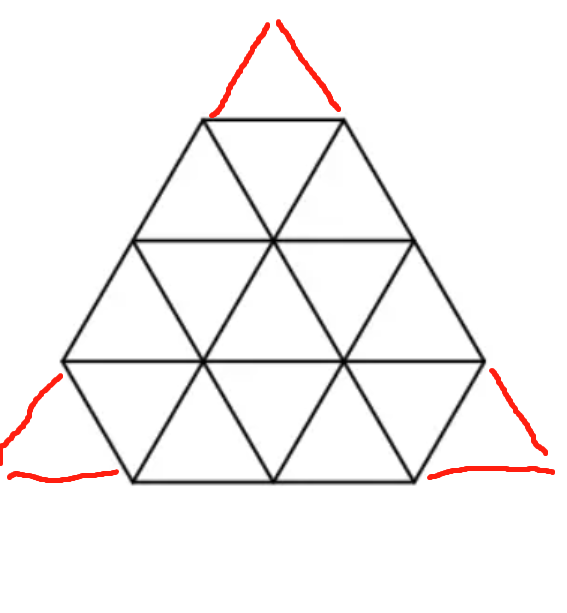
\includegraphics[width=0.86\linewidth]{assets/p7kRACD4cTf3YxK.png}\\[1pt]{\tiny\color{gray}\url{https://s2.loli.net/2023/08/17/p7kRACD4cTf3YxK.png}}\end{center}
  \item 正 $n$ 边形圆心角为 $\dfrac{360^{\circ}}{n}$ ，圆周角为 $\dfrac{180^{\circ}}{n}$ 。定义正 $n$ 边形上的三个顶点 $A,B$ 和 $C$（可以不相邻），使得 $\angle ABC=\theta$ ，当 $n\le 360$ 时，$\theta$ 可以取 $1^{\circ}$ 到 $179^{\circ}$ 间的任何一个整数 \href{https://codeforces.com/problemset/problem/1096/C}{See}。
  \item 某一点 $B$ 到直线 $AC$ 的距离公式为 $\dfrac{|\vec{BA}\times \vec{BC}|}{|AC|}$ ，等价于 $\dfrac{|aX+bY+c|}{\sqrt{a^2+b^2}}$。
  \item \texttt{atan(y / x)} 函数仅用于计算第一、四象限的值，而 \texttt{atan2(y, x)} 则允许计算所有四个象限的正反切，在使用这个函数时，需要尽量保证 $x$ 和 $y$ 的类型为整数型，如果使用浮点数，实测会慢十倍。
  \item 在平面上有奇数个点 $A_0,A_1,\dots,A_n$ 以及一个点 $X_0$ ，构造 $X_1$ 使得 $X_0,X_1$ 关于 $A_0$ 对称、构造 $X_2$ 使得 $X_1,X_2$ 关于 $A_1$ 对称、……、构造 $X_j$ 使得 $X_{j-1},X_j$ 关于 $A_{(j-1)\mod n}$ 对称。那么周期为 $2n$ ，即 $A_0$ 与 $A_{2n}$ 共点、$A_1$ 与 $A_{2n+1}$ 共点 \href{https://codeforces.com/contest/24/problem/C}{See} 。
  \item 已知 $A\ (x_A, y_A)$ 和 $X\ (x_X,y_X)$ 两点及这两点的坐标，构造 $Y$ 使得 $X,Y$ 关于 $A$ 对称，那么 $Y$ 的坐标为 $(2\cdot x_A-x_X,2\cdot y_A-y_X)$ 。
  \item \textbf{海伦公式}：已知三角形三边长 $a,b$ 和 $c$ ，定义 $p=\dfrac{a+b+c}{2}$ ，则 $S_{\triangle}=\sqrt{p(p-a)(p-b)(p-c)}$ ，在使用时需要注意越界问题，本质是铅锤定理，一般多使用叉乘计算三角形面积而不使用该公式。
  \item 棱台体积 $V=\frac{1}{3}(S_1+S_2+\sqrt{S_1S_2})\cdot h$，其中 $S_1,S_2$ 为上下底面积。
  \item 正棱台侧面积 $\frac{1}{2}(C_1+C_2)\cdot L$，其中 $C_1,C_2$ 为上下底周长，$L$ 为斜高（上下底对应的平行边的距离）。
  \item 球面积 $4\pi r^2$，体积 $\frac{4}{3}\pi r^3$。
  \item 正三角形面积 $\dfrac{\sqrt 3 a^2}{4}$，正四面体面积 $\dfrac{\sqrt 2 a^3}{12}$。
  \item 设扇形对应的圆心角弧度为 $\theta$ ，则面积为 $S=\frac{\theta}{2}\cdot R^2$ 。
\end{itemize}
\par\addvspace{2pt}\noindent\textbf{立体几何结论归档}\par
\begin{itemize}
  \item 已知向量 $\vec{r}=\{x,y,z\}$ ，则该向量的三个方向余弦为 $\cos \alpha =\dfrac{x}{|\vec r|}=\dfrac{x}{\sqrt{x^2+y^2+z^2}}; \ \cos \beta = \dfrac{y}{|\vec r|};\ \cos \gamma =\dfrac{z}{|\vec r|}$ 。其中 $\alpha,\beta,\gamma\in [0,\pi]$ ，$\cos^2\alpha+\cos^2\beta+\cos^2\gamma=1$ 。
\end{itemize}

\section{杂项}

\subsection{离散化}

\begin{lstlisting}
// 离散化
// 许多题目在处理数据的时候，并不关心值本身，只关心值之间的大小关系
// 这个时候进行离散化是比较正确的决定
template <typename T> 
vector<T> Discretization(vector<T> o_array)
{
    vector<T> knum = o_array;
    sort(knum.begin(), knum.end());
    knum.erase(unique(knum.begin(), knum.end()),knum.end());
    for(int i = 0;i<o_array.size();i++){
        o_array[i] = lower_bound(knum.begin(),knum.end(),o_array[i]) - knum.begin();
    }
    return o_array;
}
//传入一个数组，传出离散化之后的数组 如 num = Normalization(num);
\end{lstlisting}

\subsection{欧拉序（子树转区间）}

\begin{lstlisting}
//许多处理树上问题，特别是对 子树 进行操作的时候 ，往往利用欧拉序将树拍平后，再利用线段树维护
//实现了一个结构体，初始化n为节点数，并传入边（需人为确保是一棵树）
//调用成员函数.init后，会生成两个个长度为n的数组
//第一个为树的dfn序，注意默认视1为根节点
//第二个为子树索引，tp[p] 代表 p节点所在子树在dfn上对应的连续区间 ，请使用auto[lp,rp] = pt[p] 调用
struct GenerateEulerTourOrder
{
    vector<int>dfn;
    vector<pair<int,int>>tp;
    vector<vector<int>> g;
    GenerateEulerTourOrder(int n){
        dfn.reserve(n);
        tp.resize(n+1);
        g.resize(n+1);
    }
    void add(int u,int v){
        g[u].push_back(v);
        g[v].push_back(u);
    }
    void init(int head = 1){
        auto dfs = [this](auto&&self,int n,int p) ->void {
            auto & [lp,rp] = tp[n];
            dfn.emplace_back(n);
            lp = dfn.size()-1;
            for(auto nextp:g[n]){
                if(nextp== p) continue;
                else{
                    self(self,nextp,n);
                }
            }
            rp = dfn.size() - 1;
        };
        dfs(dfs,head,-1);
        return;
    }
};
\end{lstlisting}

\subsection{反转整数}

\begin{lstlisting}
// ---------- 8 位 ----------
static inline uint8_t reverse8(uint8_t x) {
    x = (uint8_t)(((x & 0x55U) << 1) | ((x & 0xAAU) >> 1));
    x = (uint8_t)(((x & 0x33U) << 2) | ((x & 0xCCU) >> 2));
    x = (uint8_t)(((x & 0x0FU) << 4) | ((x & 0xF0U) >> 4));
    return x;
}

// ---------- 16 位 ----------
static inline uint16_t reverse16(uint16_t x) {
    x = (uint16_t)(((x & 0x5555U) << 1) | ((x & 0xAAAAU) >> 1));
    x = (uint16_t)(((x & 0x3333U) << 2) | ((x & 0xCCCCU) >> 2));
    x = (uint16_t)(((x & 0x0F0FU) << 4) | ((x & 0xF0F0U) >> 4));
    x = (uint16_t)(((x & 0x00FFU) << 8) | ((x & 0xFF00U) >> 8));
    return x;
}

// ---------- 32 位 ----------
static inline uint32_t reverse32(uint32_t x) {
//            0123456789012345678901234567890123456789
    x = ((x & 0x55555555U) << 1) | ((x & 0xAAAAAAAAU) >> 1);
    x = ((x & 0x33333333U) << 2) | ((x & 0xCCCCCCCCU) >> 2);
    x = ((x & 0x0F0F0F0FU) << 4) | ((x & 0xF0F0F0F0U) >> 4);
    x = ((x & 0x00FF00FFU) << 8) | ((x & 0xFF00FF00U) >> 8);
    x = ((x & 0x0000FFFFU) << 16) | ((x & 0xFFFF0000U) >> 16);
    return x;
}

// ---------- 64 位 ----------
static inline uint64_t reverse64(uint64_t x) {
    //        012345678901234567890123456789012345678901234567890123456789
    x = ((x & 0x5555555555555555ULL) << 1) | ((x & 0xAAAAAAAAAAAAAAAAULL) >> 1);
    x = ((x & 0x3333333333333333ULL) << 2) | ((x & 0xCCCCCCCCCCCCCCCCULL) >> 2);
    x = ((x & 0x0F0F0F0F0F0F0F0FULL) << 4) | ((x & 0xF0F0F0F0F0F0F0F0ULL) >> 4);
    x = ((x & 0x00FF00FF00FF00FFULL) << 8) | ((x & 0xFF00FF00FF00FF00ULL) >> 8);
    x = ((x & 0x0000FFFF0000FFFFULL) << 16) | ((x & 0xFFFF0000FFFF0000ULL) >> 16);
    x = ((x & 0x00000000FFFFFFFFULL) << 32) | ((x & 0xFFFFFFFF00000000ULL) >> 32);
    return x;
}

// ---------- 128 位 ----------
static inline unsigned __int128 reverse128(unsigned __int128 x) {
    uint64_t lo = (uint64_t)x;                 // 低 64 位
    uint64_t hi = (uint64_t)(x >> 64);         // 高 64 位
    // 翻转整个 128 位：低块翻转后移到高位，高块翻转后移到低位
    return ((unsigned __int128)reverse64(lo) << 64) | reverse64(hi);
}
//有符号数，直接借用无符号数
static inline int8_t  reverse_int8 (int8_t  x) { return (int8_t) reverse8 ((uint8_t) x);  }
static inline int16_t reverse_int16(int16_t x) { return (int16_t)reverse16((uint16_t)x); }
static inline int32_t reverse_int32(int32_t x) { return (int32_t)reverse32((uint32_t)x); }
static inline int64_t reverse_int64(int64_t x) { return (int64_t)reverse64((uint64_t)x); }
static inline __int128 reverse_int128(__int128 x) {
    return (__int128)reverse128((unsigned __int128)x);
}
\end{lstlisting}

\subsection{防卡哈希表}

\begin{lstlisting}
#include <bits/stdc++.h>
using namespace std;
using ull = unsigned long long;
#include <ext/pb_ds/assoc_container.hpp>
#include <ext/pb_ds/tree_policy.hpp>
struct chash {
    static ull splitmix64(ull x) {
        x += 0x9e3779b97f4a7c15;
        x = (x ^ (x >> 30)) * 0xbf58476d1ce4e5b9;
        x = (x ^ (x >> 27)) * 0x94d049bb133111eb;
        return x ^ (x >> 31);
    }

    size_t operator()(ull x) const {
        static const ull F = 
            chrono::steady_clock::now().time_since_epoch().count();
        return splitmix64(x + F);
    }
};
template<typename K, typename V>
using HashMap = __gnu_pbds::gp_hash_table<K, V, chash>;
\end{lstlisting}


\end{multicols}

\end{document}
